% Preamble for the DM notes.
% This is shared between main.tex and the temporary document we use on
% writelatex.com.
\documentclass[10pt,a4paper,titlepage,oneside,final]{book}
\usepackage[english]{babel}
\usepackage[utf8x]{inputenc}
\usepackage[T1]{fontenc}
\usepackage{calc}
\usepackage{lmodern}
\usepackage{pifont}
\usepackage[a4paper,textwidth=345pt,textheight=598pt,hmarginratio=1:1]{geometry}
\usepackage[final]{graphicx}
\usepackage{subfigure}
\usepackage[intlimits]{amsmath}
\usepackage{amssymb}
\usepackage{booktabs}
\usepackage{microtype}
\usepackage{float}
\usepackage{framed}
\usepackage{cleveref}
\usepackage{tabularx}
\usepackage{caption}
\usepackage{ragged2e}
\usepackage{soul}
\usepackage{theorem}
\usepackage{tikz}
\usepackage{makeidx}
\usepackage{paralist}
\usepackage[iso,german,english]{isodate}
\usepackage{placeins}
\usepackage[pdfborder={0 0 0}]{hyperref}

\newcommand{\AuthorOne}{Patrik Fimml}
\newcommand{\AuthorTwo}{NeroBurner}
\newcommand{\AuthorThree}{emptyvi}
\newcommand{\AuthorFour}{fbr}
\newcommand{\AuthorFive}{gsp}
\newcommand{\AuthorSix}{mgh33}
\newcommand{\AuthorSeven}{sanssecours}
\newcommand{\AuthorEight}{Tidon}

\newcommand{\Title}{Lecture Notes 2013W}
\newcommand{\Subject}{104.271 Discrete Mathematics VO}
\newcommand{\Keywords}{Graph Theory, Combinatorics}

\definecolor{aqua}{rgb}{0, 0.56, 1}

% Hyperref properties
\hypersetup
{
  pdftitle    = {\Title},
  pdfsubject  = {\Subject},
  pdfauthor   = {\AuthorOne, \AuthorTwo, \AuthorThree, \AuthorFour,
                 \AuthorFive, \AuthorSix, \AuthorSeven, \AuthorEight},
  pdfkeywords = {\Keywords},
  colorlinks  = true,
  linkcolor   = black,
  anchorcolor = black,
  citecolor   = grey,
  urlcolor    = orange
}

\makeatletter

\captionsetup{format=hang,justification=justified,labelfont=bf,labelsep=colon,font=small}
\long\def\clap#1{\hbox to 0pt{\hss#1\hss}}

\author{\AuthorOne \and \AuthorTwo \and \AuthorThree \and \AuthorFour \and
        \AuthorFive \and \AuthorSix \and \AuthorSeven \and \AuthorEight}
\title{\Title\\ \Subject\\ (Gittenberger)}
\def\@thanks{%
  \vfill%
  \textbf{Collaborate!} This document is edited collaboratively. We take notes
  during the lecture using EtherPad, and maintain them afterwards using Git.
  Join us! \mbox{\href
    {http://www.informatik-forum.at/showthread.php?104454-Notes-2013WS-VO_01&p=809709&viewfull=1\#post809709}
    {\nolinkurl{http://informatik-forum.at/showthread.php?104454-Notes-2013WS}}}
}

\makeindex
\gdef\th@custom{%
  \th@plain%
  \def\@begintheorem##1##2{%
    \item[\hskip\labelsep \theorem@headerfont ##1\ ##2.]}}%
\theoremstyle{custom}
\theorembodyfont{\normalfont}
\newtheorem{definition}{Definition}

\def\thechapter{\Roman{chapter}}

\parindent=0pt
\parskip=\medskipamount

\pltopsep=-5pt
\plpartopsep=0pt

\newcommand{\TODO}[1]{
  \begin{framed}
    TODO: {#1}
  \end{framed}}

\newcommand{\tikzmark}[2]{\tikz[overlay,remember picture,baseline] \node [anchor=base] (#1) {$#2$};}

\newcommand{\DrawLineHorizontal}[3][]{%
	\begin{tikzpicture}[overlay,remember picture]
		\draw[#1] (#2.west) -- (#3.east);
	\end{tikzpicture}
}
\newcommand{\DrawLine}[3][]{%
	\begin{tikzpicture}[overlay,remember picture]
		\draw[#1] (#2.north) -- (#3.south);
	\end{tikzpicture}
}

% "defined term"
\def\dt#1{\textbf{#1}}

\def\Remark.{\noindent \textbf{Remark.}}
\def\Lemma.{\noindent \textbf{Lemma.}}
\def\Theorem.{\noindent \textbf{Theorem.}}
\def\Proof.{\noindent \textbf{Proof.}}
\def\ProofForward.{\noindent \textbf{Proof (``$\Rightarrow$'').}}
\def\ProofBackward.{\noindent \textbf{Proof (``$\Leftarrow$'').}}

\newcommand\lecturedate[2][0pt]{%
  \marginpar{%
    \raisebox{2pt+#1}{%
      \vbox{%
        \rule{5em}{.4pt} \\[0pt]%
        \hspace*{1pt}%
        \scriptsize%
        \printdate{#2}%
      }%
    }%
  }%
  \ignorespaces%
}

\def\missingdate#1{%
  \par\strut\lecturedate{#1}%
  \TODO{Missing content from \printdate{#1}}%
  \par%
}

\isodash{--}

\def\@path#1,{#1\@ifnextchar\relax{}{\text{---}\@path}}
\def\path#1{\ensuremath{\@path#1,\relax}}

\DeclareMathOperator{\seq}{seq}
\DeclareMathOperator{\cyc}{cyc}
\DeclareMathOperator{\set}{set}
\DeclareMathOperator{\ord}{ord}
\DeclareMathOperator{\lcm}{lcm}

\def\GroupGenBy#1{\left\langle #1 \right\rangle}



% Put all options specific to the main document here. Anything that applies
% both to the main document and WriteLaTeX belongs in dmpreamble.tex.

% this file contains tikz-makros

% counter for numbering the nodes
\newcounter{nodecount}
% #1 ... list of degrees, where the nodes are placed
% #2 ... radius of the node-placement
\def \fullyConnectedGraph #1#2{%
  \setcounter{nodecount}{0}
  \foreach \x in {#1} 
  {
    \stepcounter{nodecount}
    \node (n\the\value{nodecount}) at (\x:#2) {};
  };
  \foreach \i in {1,...,\the\value{nodecount}} 
  {
    \fill (n\i) circle(2pt);
    \foreach \j in {\i,...,\the\value{nodecount}}
    {
      \path (n\i) edge (n\j);
    };
  };%
}

% draw a graph
% #1 ... list of x/y coordinates for the nodes
% #2 ... list of pahtes between nodes, beginning with 1
\def \drawGraph #1#2{%
  \setcounter{nodecount}{0}
  \foreach \x/\y in {#1} {
    \stepcounter{nodecount}
    \node (n\the\value{nodecount}) at (\x,\y) {};
    \fill (n\the\value{nodecount}) circle(2pt);
  };
  \foreach \i/\j in {#2} {
    \path (n\i) edge (n\j);
  };
}

% draw a directed graph
% #1 ... list of x/y coordinates for the nodes
% #2 ... list of pahtes between nodes, beginning with 1
\def \drawDirGraph #1#2{%
  \setcounter{nodecount}{0}
  \foreach \x/\y in {#1} {
    \stepcounter{nodecount}
    \node (n\the\value{nodecount}) at (\x,\y) {};
    \fill (n\the\value{nodecount}) circle(2pt);
  };
  \foreach \i/\j in {#2} {
    \path (n\i) edge[->] (n\j);
  };
}



\makeindex

\begin{document}

\maketitle
\tableofcontents
%\listoffigures

% include the chapters here:

\chapter{Graph Theory}
%%%  03.10.2013  %%%
%%%  VO 01
\section{Basics}
\lecturedate[\baselineskip]{2013-10-03}

\begin{definition}
\index{graph}
\index{vertex set}
\index{edge set}
A structure \dt{$G=(V,E)$} is called a \dt{graph}.
$V=\{v_1, v_2, \ldots, v_n\}$ is the \emph{vertex set} of $G$. $E$ is the
\emph{edge set} of $G$.
\end{definition}

\begin{definition}
\index{graph!directed}
\index{edge}
A \dt{directed graph} $G$ has directed edges $e\in E$ of the form
$e=(v,w)$. $e$ is a pair, in particular $(v,w)\ne (w,v)$. $v,w\in V$.
\end{definition}

\begin{definition}
\index{graph!undirected}
\index{edge}
An \dt{undirected graph} $G$ has undirected edges $e\in E$ of the form
$e=\{v,w\}$. $e$ is a set, in particular $e=\{v,w\}=\{w,v\}=vw$. $vw$ is a
shorthand notation.
\end{definition}

\index{loop}
A \dt{loop} is an edge from a vertex to itself.

Graphs can have \textbf{multiple edges}, in which case $E$ is a multiset.

\begin{figure}[htb]
\centering
\begin{tabular}{c c}
\subfigure[directed graph] {
	
\includegraphics[scale=.5]{01_graph_theory/pics/directed-graph_edge.pdf}
} &
\subfigure[undirected graph] {
	
\includegraphics[scale=.5]{01_graph_theory/pics/graph_edge.pdf}
} \\
\subfigure[loop] {
	
\includegraphics[scale=.5]{01_graph_theory/pics/graph_loop.pdf}
} &
\subfigure[multiple edges] {
	
\includegraphics[scale=.5]{01_graph_theory/pics/graph_multiple-edges.pdf}
}
\end{tabular}
\caption{different graphs}
\end{figure}
\FloatBarrier

\begin{definition}
\index{graph!simple}
A graph is \dt{simple} when it has
\begin{compactitem}
\item no loops and 
\item no multiple edges.
\end{compactitem}
\end{definition}

Unless otherwise stated, we assume simple, finite graphs throughout this
lecture.

A graph corresponds to a \emph{relation} on $V$. In case of undirected graphs,
this relation is symmetric.


Notation: \\[\medskipamount]
\begin{tabular}{ll}
  $V$, $V(G)$ & vertice set \\
  $E$, $E(G)$ & edge set \\
  $\alpha_0 = |V|$ & number of vertices \\
  $\alpha_1 = |E|$ & number of edges \\
\end{tabular}

\begin{definition}
\index{degree}
Let $v\in V$. For undirected graphs, 
\begin{compactitem}
  \item the \dt{degree} $d(v)$ is the number of edges \emph{incident} to $v$.
\end{compactitem}
For directed graphs,
\begin{compactitem}
  \item the \dt{out-degree} $d^{+}(v)$ is the number of outgoing edges, i.e. edges of the form $(v,w)$, and
  \item the \dt{in-degree} $d^{-}(v)$ is the number of incoming edges, i.e. edges of the form $(w,v)$.
\end{compactitem}
\end{definition}

\begin{figure}[htb]
\centering
\subfigure[vertex $v$ with degree $d(v)=6$]{
	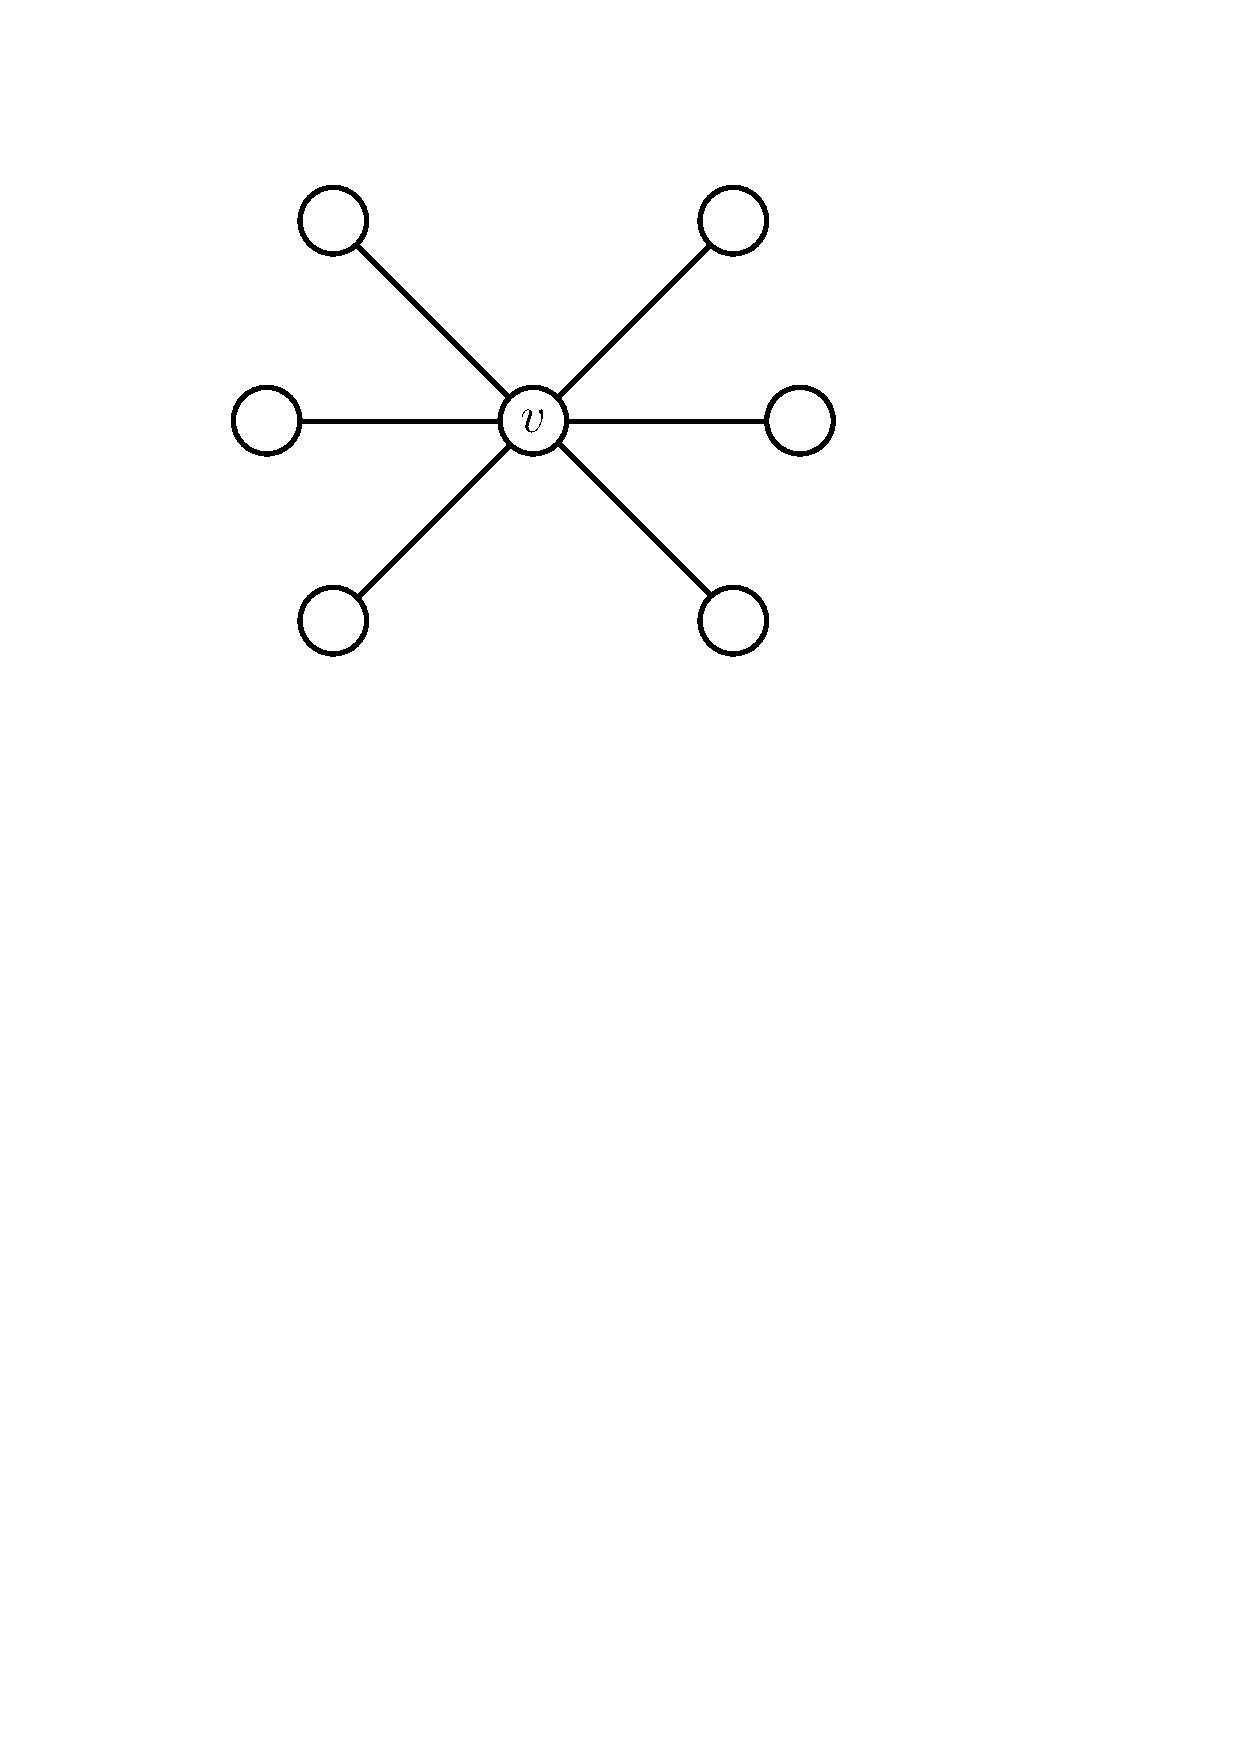
\includegraphics[scale=.5]{01_graph_theory/pics/graph_degree.pdf}
}
\subfigure[vertex $v$ with in-degree $d^{-}(v)=3$ and out-degree $d^{+}(v)=3$]{
	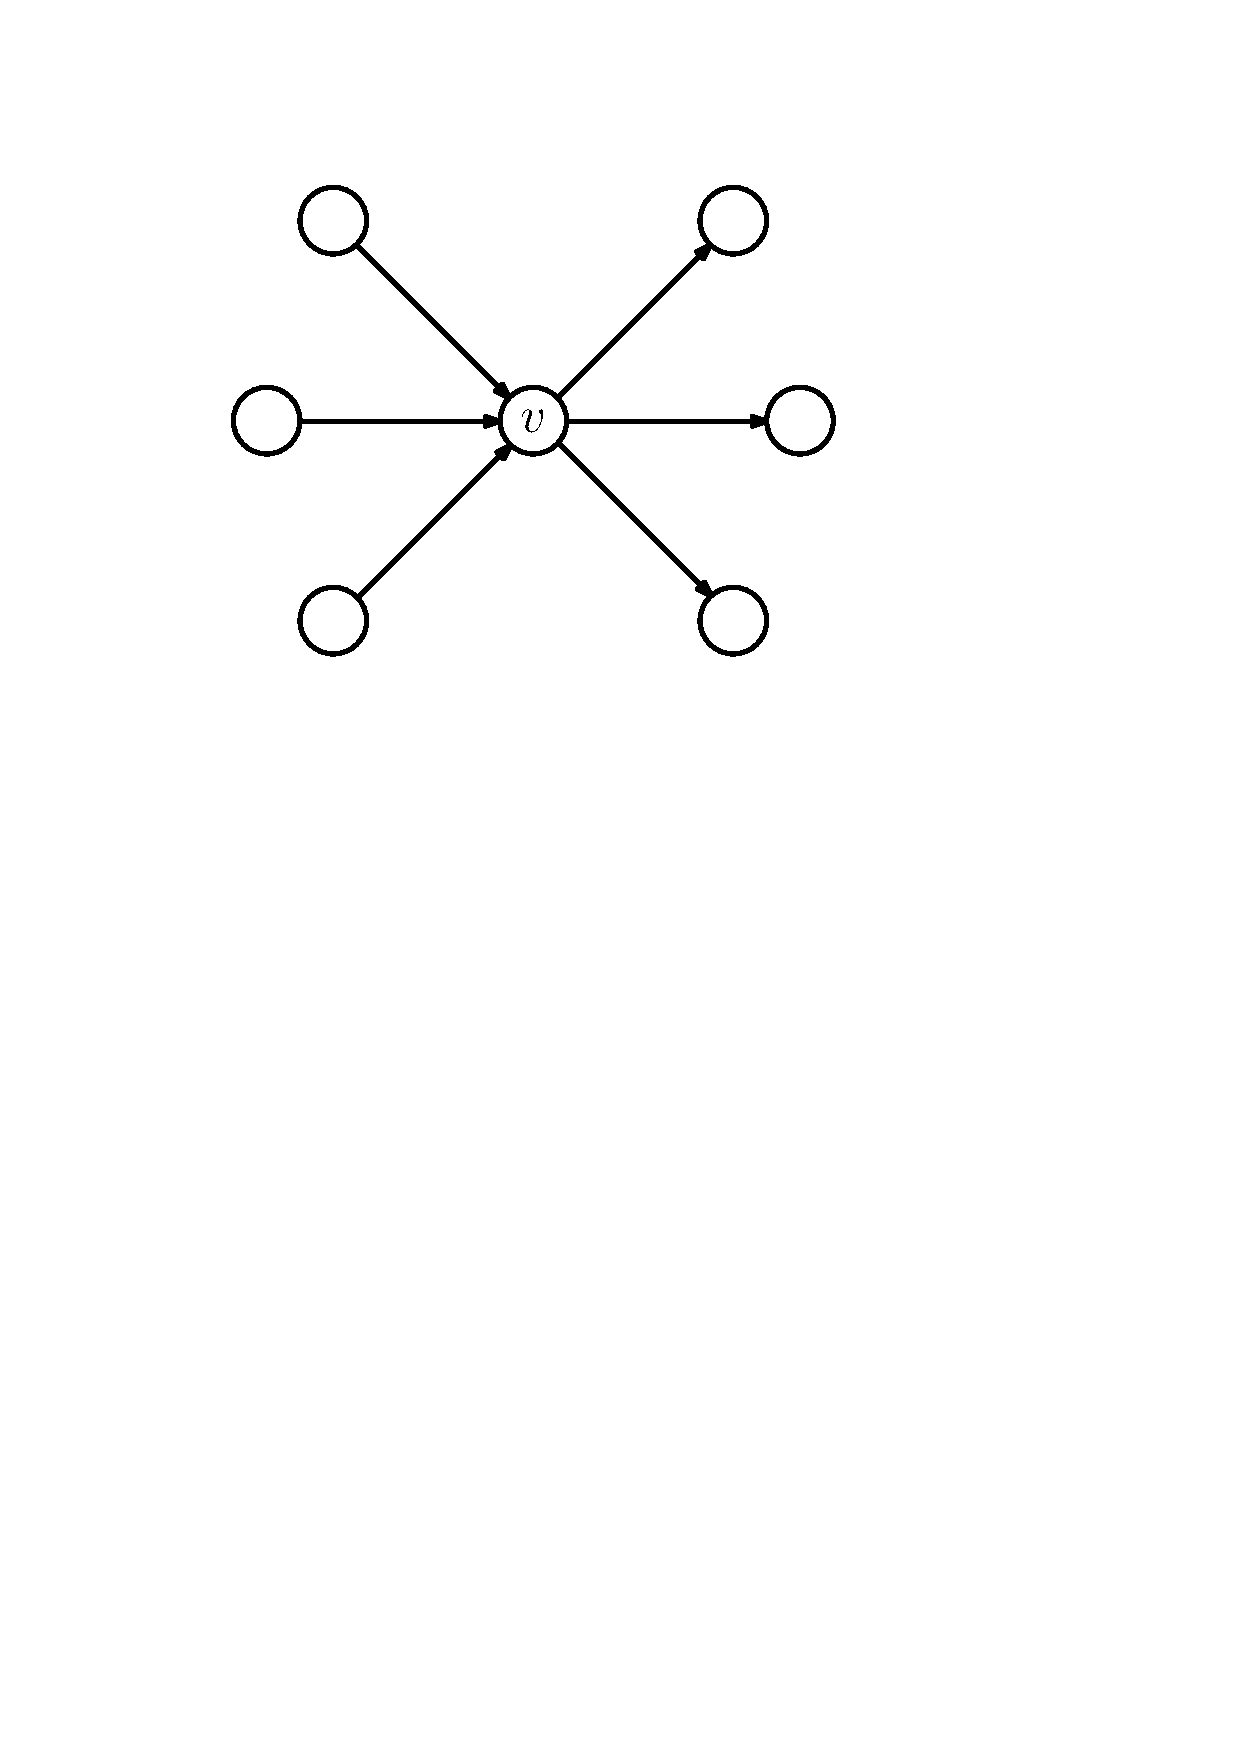
\includegraphics[scale=.5]{01_graph_theory/pics/directed-graph_indegree-outdegree.pdf}
}
\caption{vertex-degrees}
\end{figure}
\FloatBarrier

\begin{definition}
\index{neighbour}
\index{successor}
\index{predecessor}
For undirected graphs,
\begin{compactitem}
\item $\Gamma(v)$ is the \dt{set of neighbours} of $v$.
\end{compactitem}
For directed graphs,
\begin{compactitem}
\item $\Gamma^{+}(v)$ is the \dt{set of successors} of $v$.
\item $\Gamma^{-}(v)$ is the \dt{set of predecessors} of $v$.
\end{compactitem}
\end{definition}

\index{handshaking lemma}
\textbf{Lemma (Handshaking Lemma).} Let $G=(V,E)$ be a simple graph. Then
\begin{align*}
&\sum_{v\in V} d(v) = 2 |E| &&\text{($G$ undirected)} \\
&\sum_{v\in V} d^{+}(v) = \sum{v\in V} d^{-}(v) = |E| &&\text{($G$ directed).} \\
\end{align*}

\textbf{Proof.} see Figure~\ref{fig:hand_shaking_lemma}

\begin{figure}[htb]
\centering
\subfigure[undirected graph, each edge is counted twice]{
	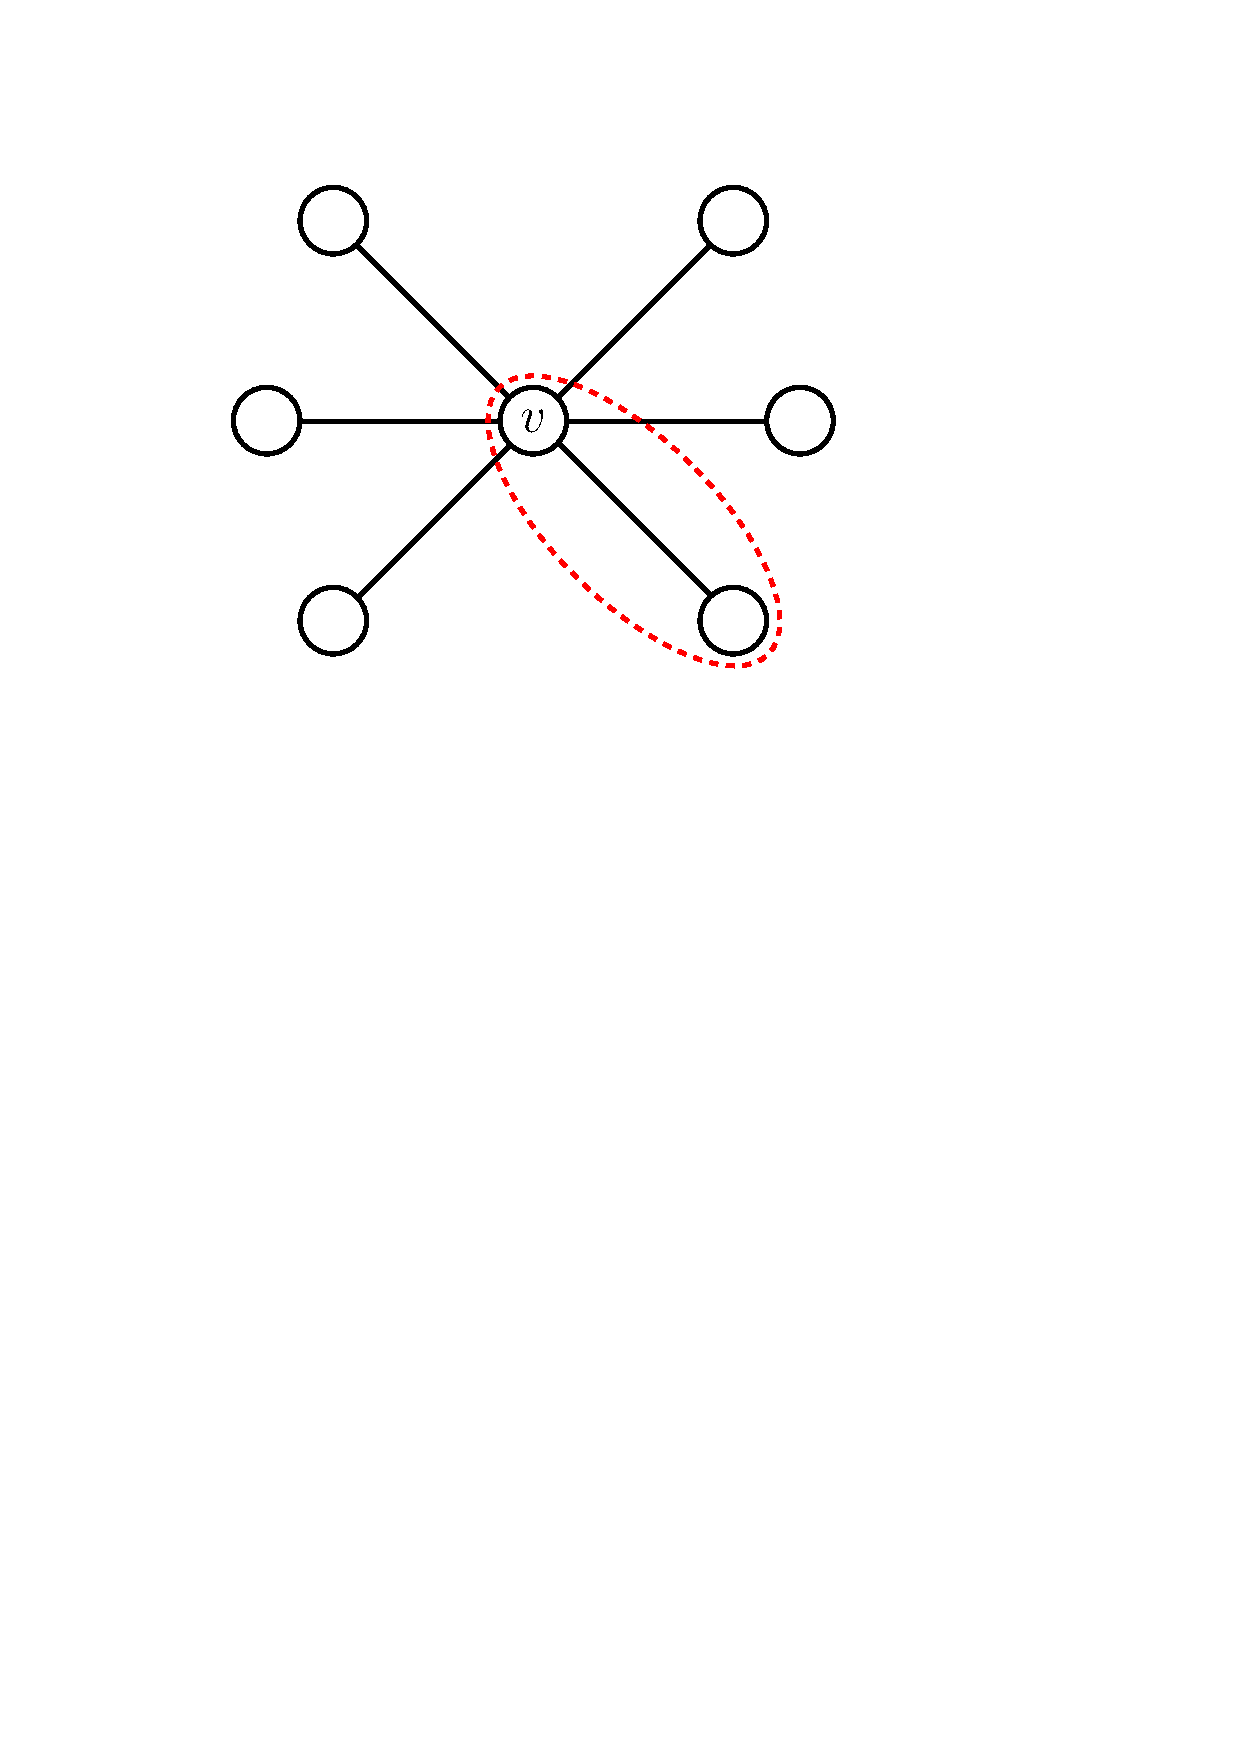
\includegraphics[scale=.5]{01_graph_theory/pics/graph_degree_handshaking-lemma.pdf}
}
\subfigure[directed graph, each edge is counted only once]{
	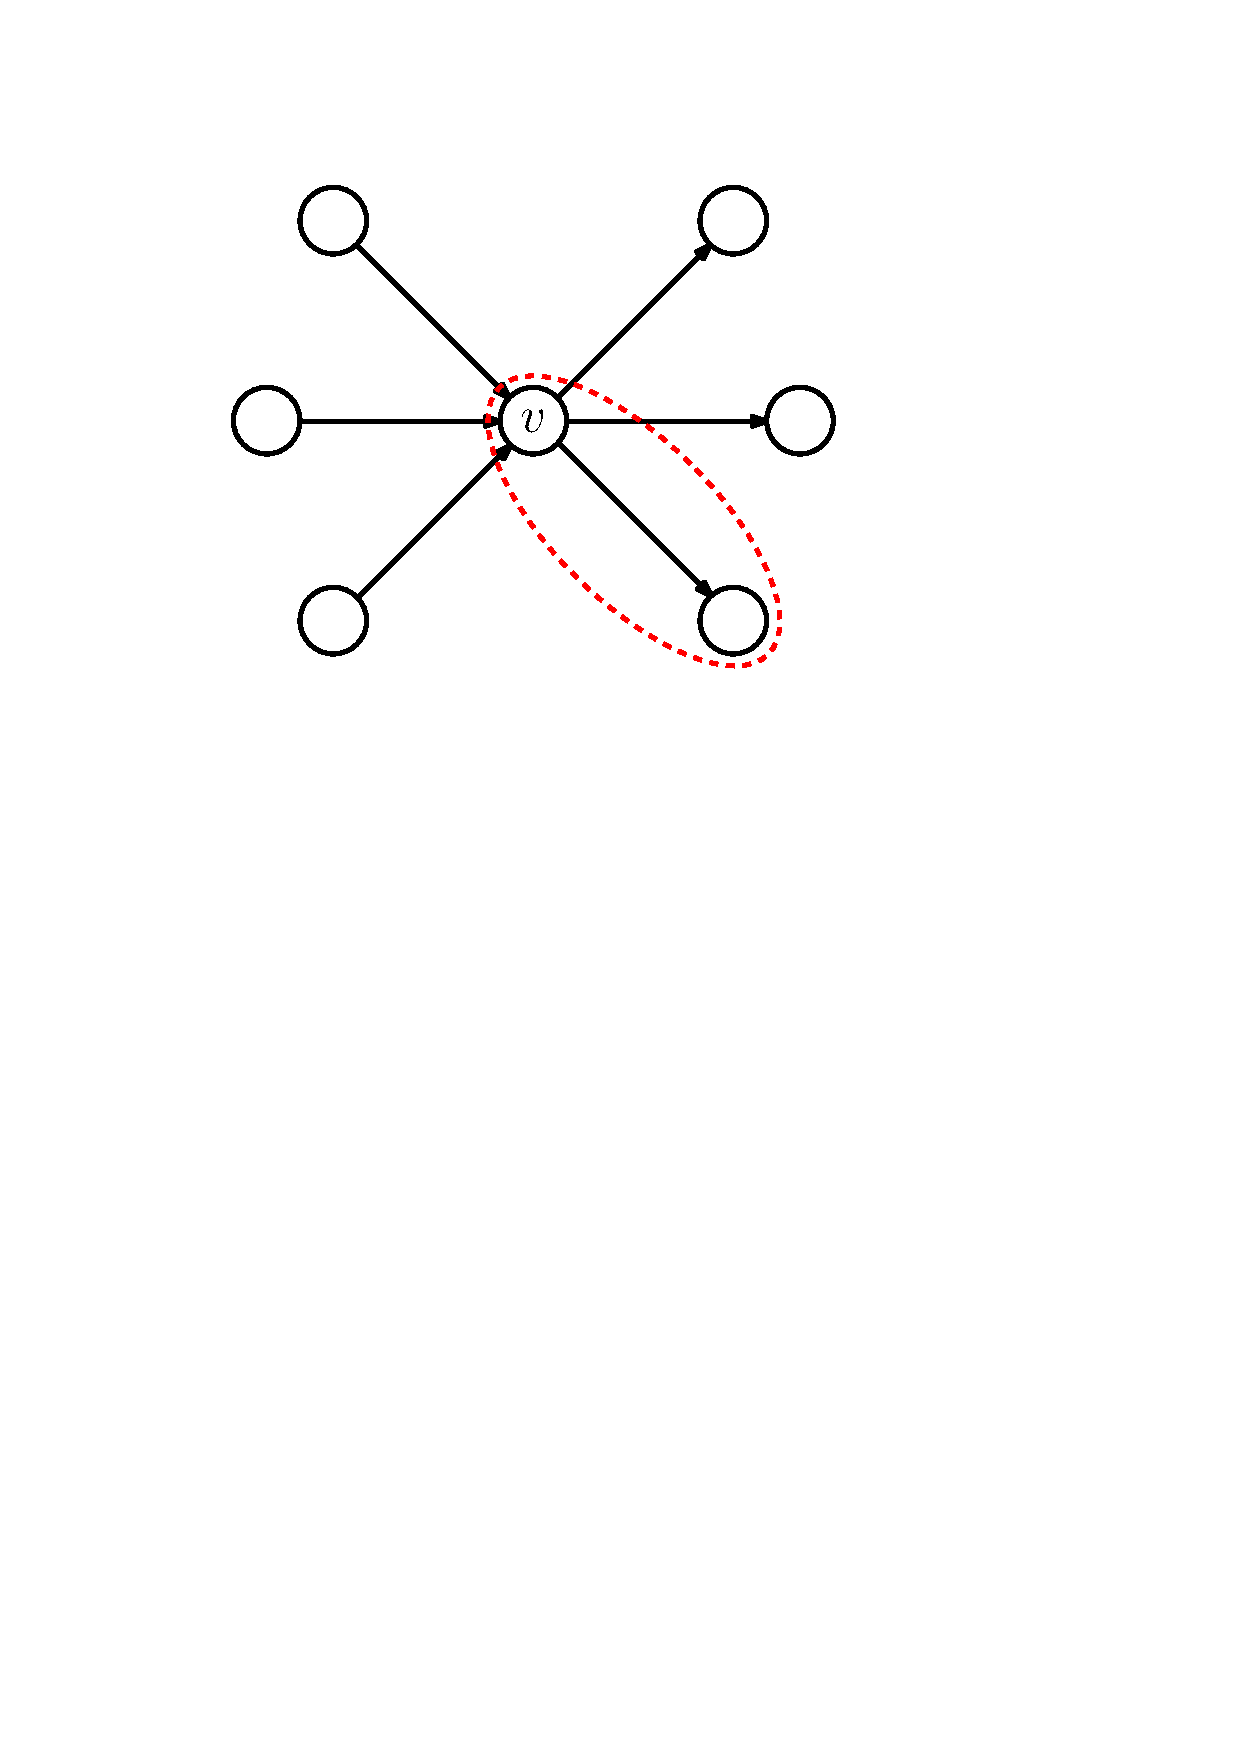
\includegraphics[scale=.5]{01_graph_theory/pics/directed-graph_degree_handshaking-lemma.pdf}
}
\caption{Hand Shaking Lemma in undirected and directed graphs}
\label{fig:hand_shaking_lemma}
\end{figure}
\FloatBarrier

\textbf{Example (Hypercube).} 
$G = (\{0,1\}^n, E)$

$vw \in E \Leftrightarrow \sum_{i=1}^{n} |v_i - w_i | = 1$ (only one switch in coordinates)

$v = v_1, v_2, \ldots , v_n$\\
$w = w_1, w_2, \ldots , w_n$

compute $a_0$ and $a_1$

$a_0 = 2^n$ \\
$a_1 = \frac{1}{2} \sum_{v \in V} d(v) = 2^{n-1} * n$

$d(v) = n \Rightarrow $ regular Graph
\begin{figure}[htb]
\centering
\subfigure[1D-hypercube]{
	
\includegraphics[scale=.4]{01_graph_theory/pics/1D-cube.pdf}
}
\subfigure[2D-hypercube]{
	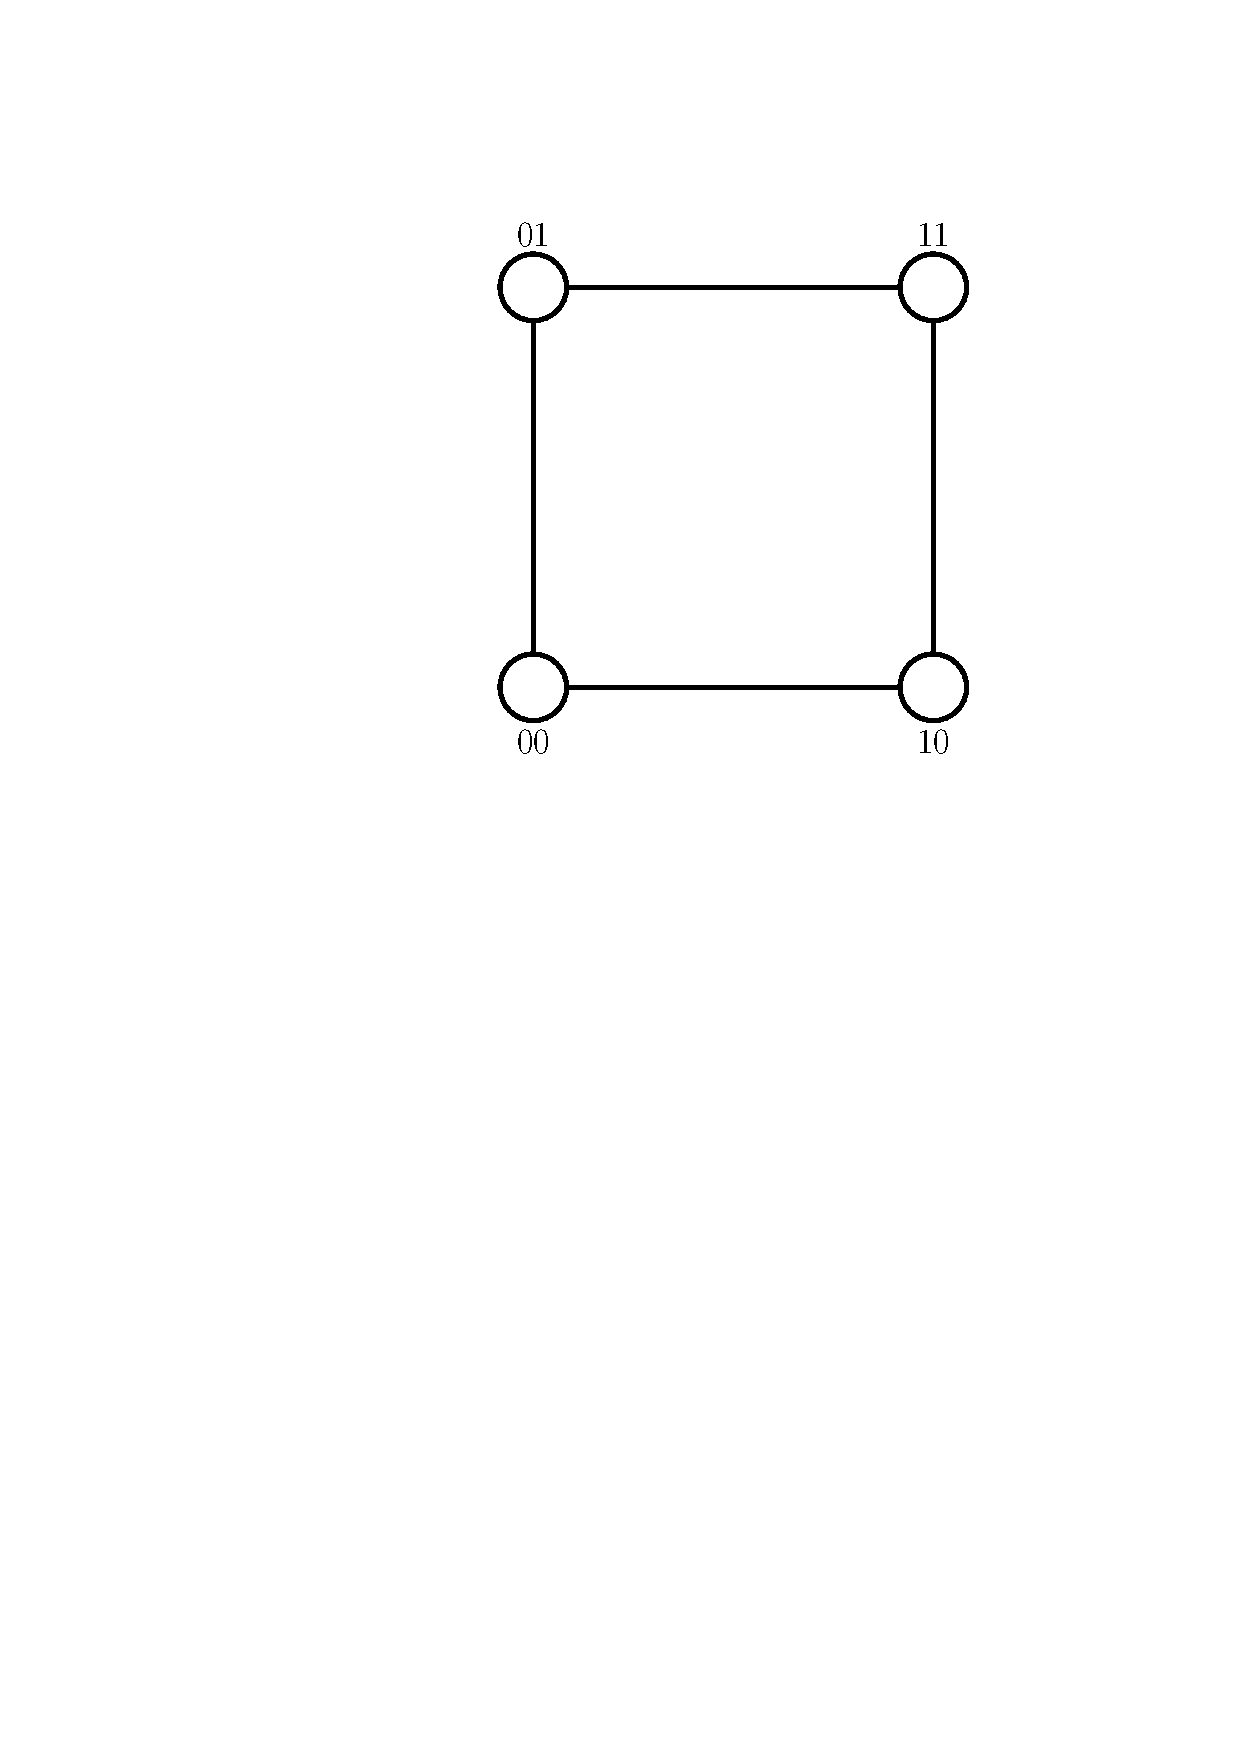
\includegraphics[scale=.4]{01_graph_theory/pics/2D-cube.pdf}
}
\subfigure[3D-hypercube]{
	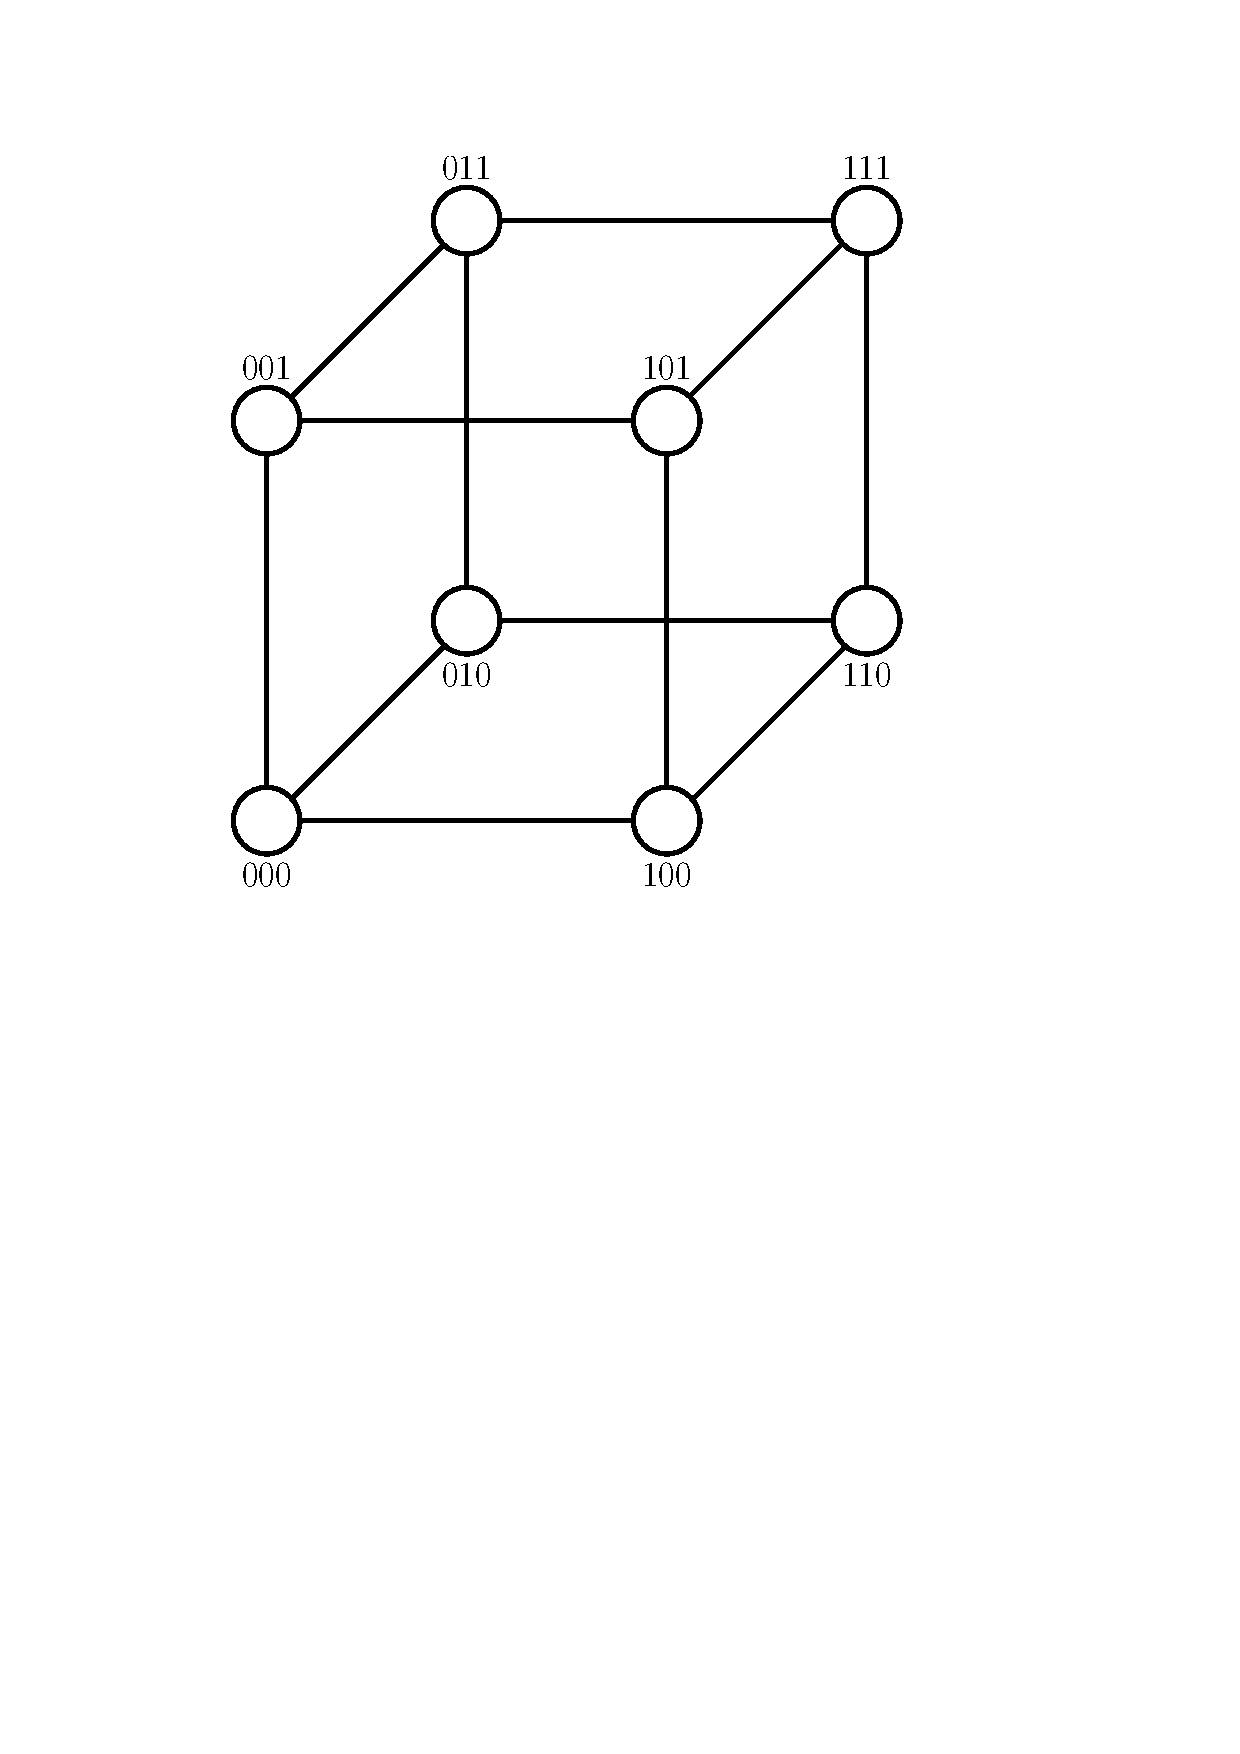
\includegraphics[scale=.4]{01_graph_theory/pics/3D-cube.pdf}
}
\caption{n-Hypercubes}
\end{figure}
\FloatBarrier

\begin{definition}
\index{adjacency}
\index{incidence}
Let $e=vw\in E$. Then we say that
\begin{compactitem}
\item $v$ and $w$ are \dt{adjacent} ($v\sim w$), and
\item $e$ and $v$ are \dt{incident} (as well as $e$ and $w$).
\end{compactitem}
\end{definition}

\begin{definition}
\index{adjacency!matrix}
Let $V=\{v_1,\ldots,v_n\}.$ The \dt{adjacency matrix} $A =
(a_{ij})_{i,j=1,\ldots,n}$ consists of entries
\[
  a_{ij} = \begin{cases}
    1 & v_i\sim v_j\text{ ($v_i$ and $v_j$ adjacent)} \\
    0 & v_i\not\sim v_j
  \end{cases}
\]
\end{definition}

\begin{figure}[htb]
\centering
\subfigure[adjacency $k = 1$]{
	
\includegraphics[scale=.5]{01_graph_theory/pics/adjacency_k-1.pdf}
}
\subfigure[adjacency $k = 2$]{
	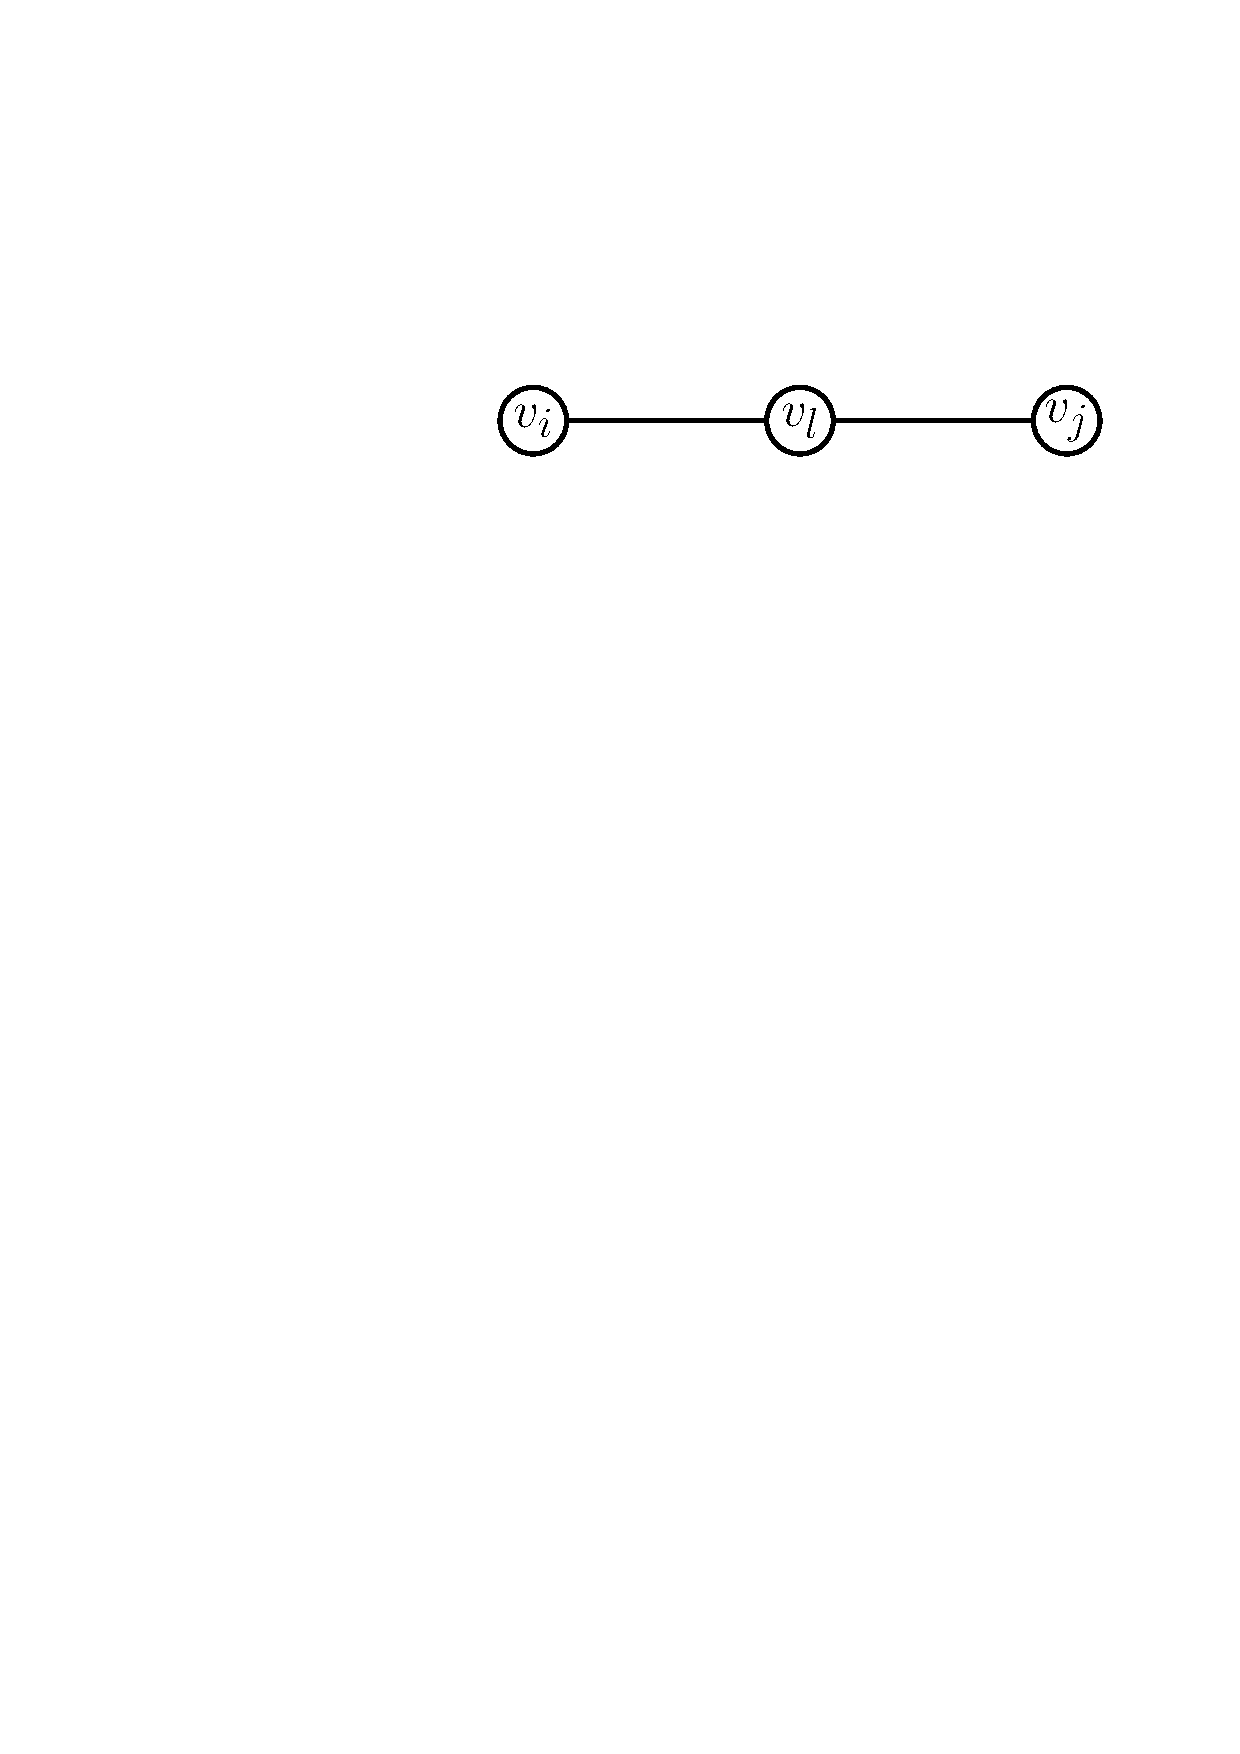
\includegraphics[scale=.5]{01_graph_theory/pics/adjacency_k-2.pdf}
}
\subfigure[adjacency via induction]{
	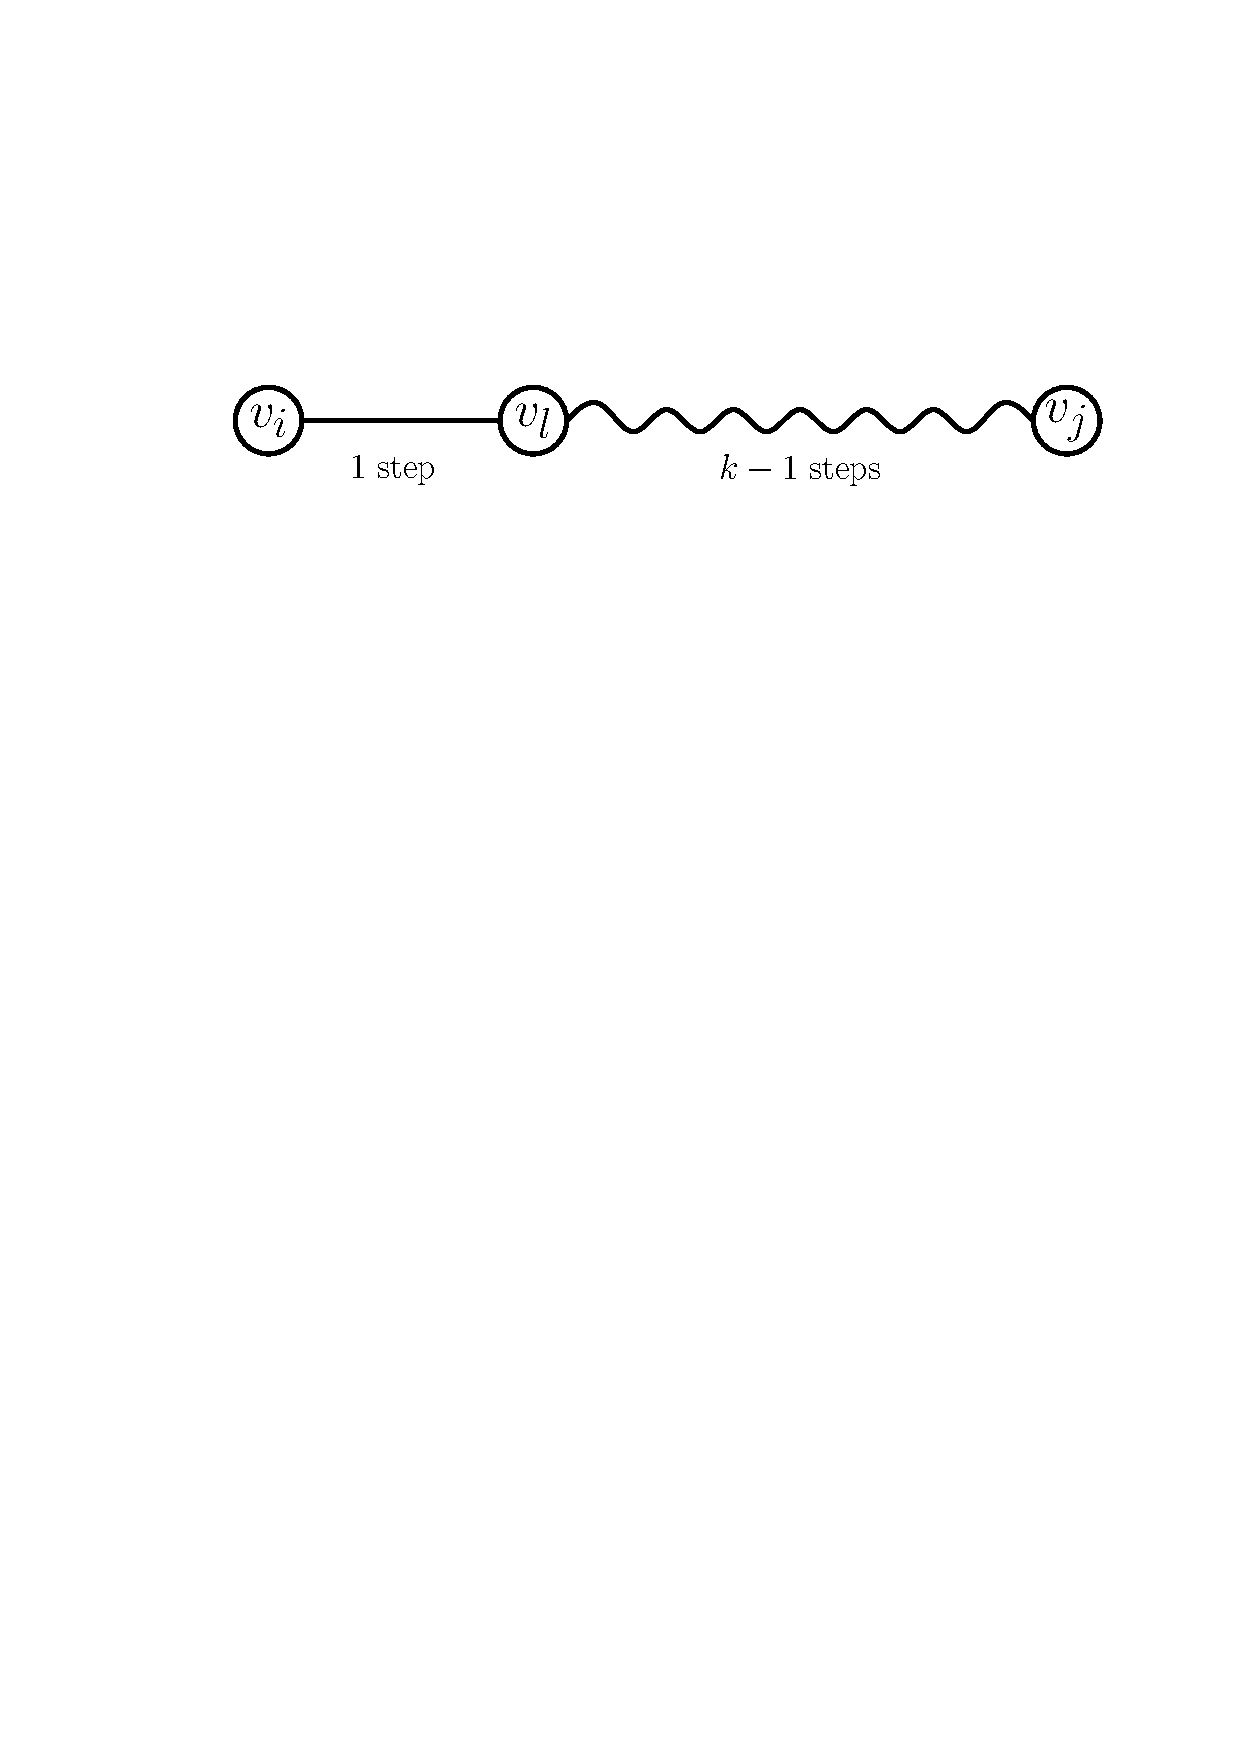
\includegraphics[scale=.5]{01_graph_theory/pics/adjacency_k-induction.pdf}
}
\caption{adjaceny}
\end{figure}
\FloatBarrier

\textbf{Remark.} If $G$ is undirected, $A$ is symmetric.

\textbf{Remark.} Consider
\begin{align*}
A^k &= (a_{ij}^{[k]})_{i,j=1,\ldots,n} = A\cdot A^{k-1} \\
a_{ij}^{[k]} &= \sum_{l=1}^n a_{il}^{\vphantom{[k-1]}}\cdot a_{lj}^{[k-1]}.
\end{align*}
The entries $a_{ij}^{[k]}$ of $A^k$ give the number of ways to get from $v_i$ to $v_j$ in exactly $k$ steps.

\begin{definition}
\index{walk}
A \dt{walk} in a graph $G$ is a sequence of edges, where successive edges have
a vertex in common. Edges can appear multiple times.
\end{definition}

\begin{figure}[htb]
\centering
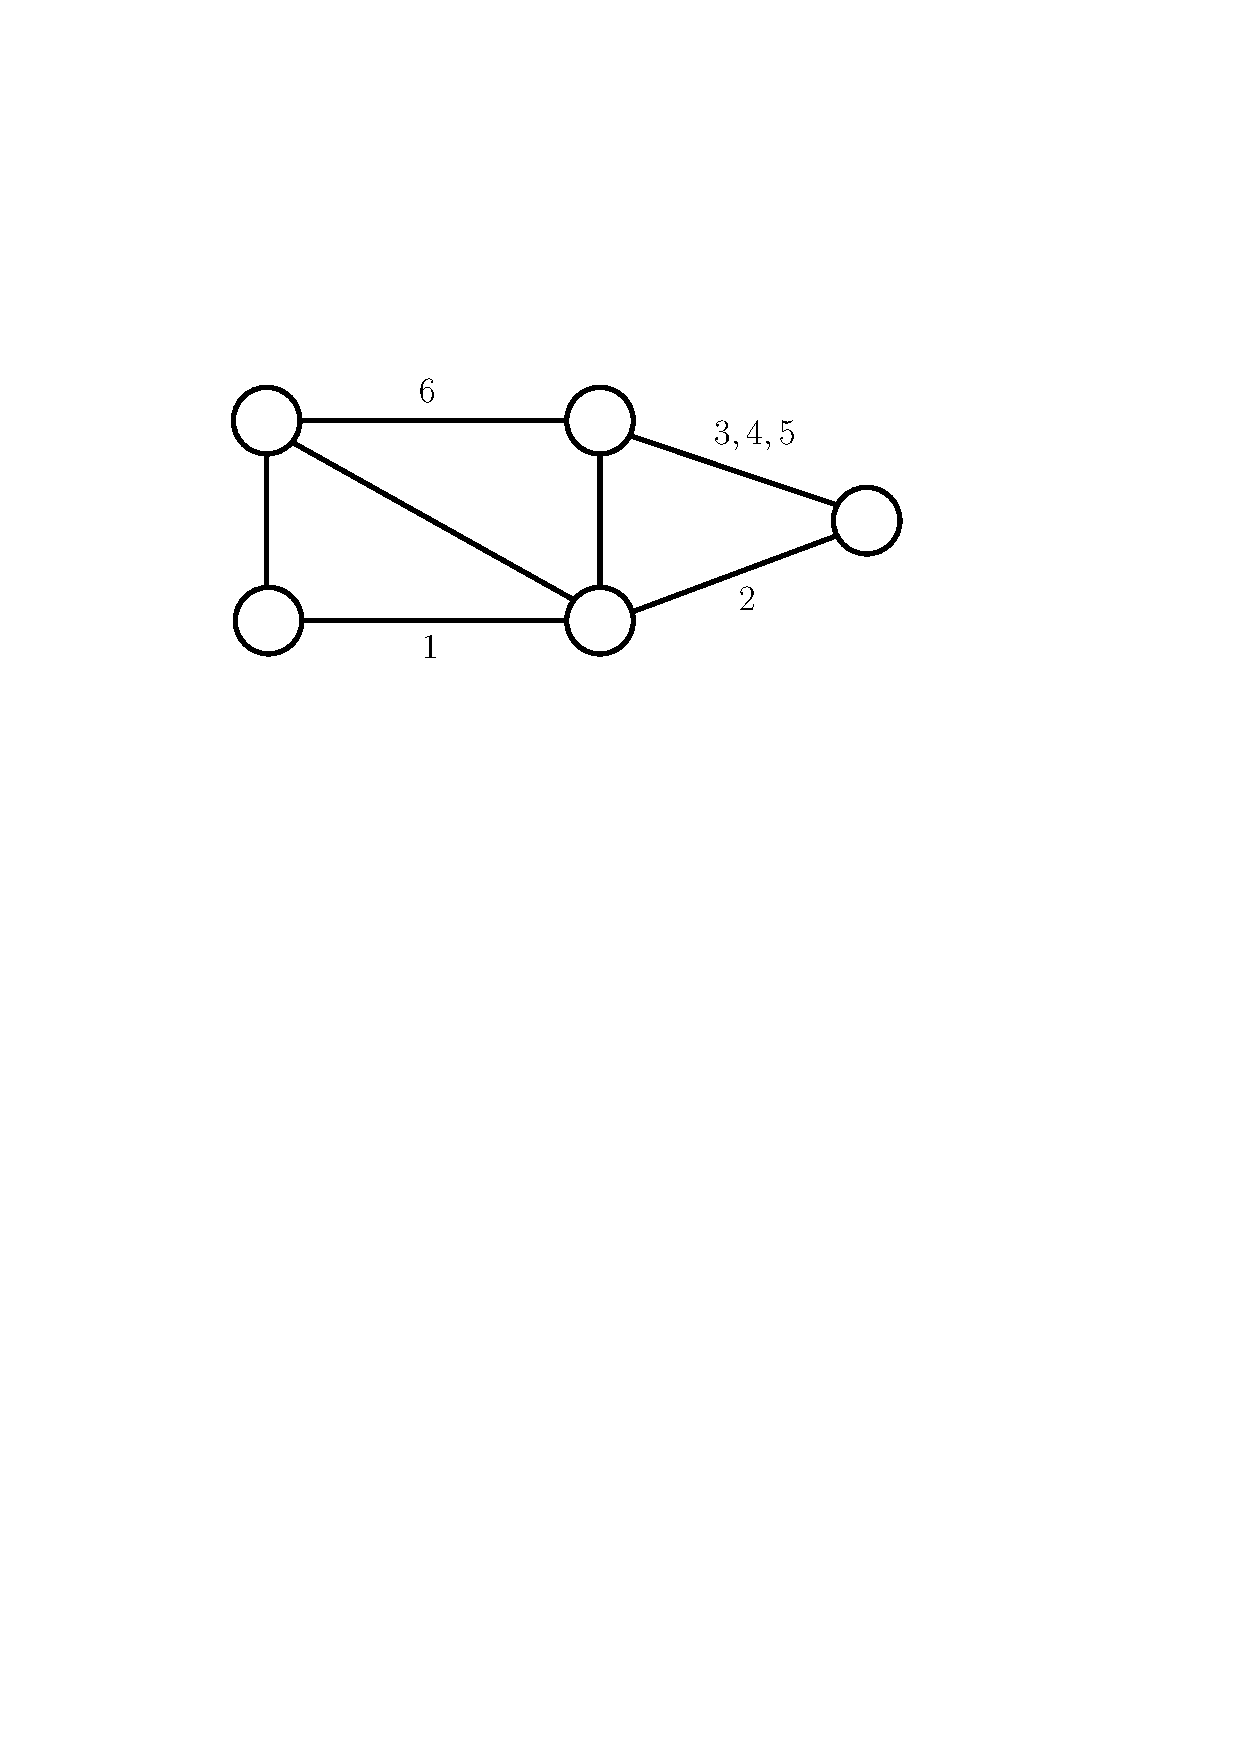
\includegraphics[scale=.5]{01_graph_theory/pics/walk.pdf}
\caption{Example of a walk through a graph}
\end{figure}
\FloatBarrier

\begin{definition}
\index{trail}
\index{circuit}
A \dt{trail} is a walk without repeated edges. A \dt{closed trail} or
\dt{circuit} starts and ends at the same vertex.
\end{definition}

\begin{definition}
\index{subgraph}
Let $G=(V,E)$. $H=(V',E')$ is a \dt{subgraph} of $G$ ($H \leq G$) if
\begin{compactitem}
\item $H$ is a graph,
\item $V' \subseteq V$, and
\item $E' \subseteq E$.
\end{compactitem}
$E'$ only contains edges between vertices in $V'$, this is implied by the requirement that $H$ is a graph.
\end{definition}

\begin{definition}
\index{connectivity}
\index{relation!connectivity relation}
For undirected graphs, we define the \dt{connectivity relation} $\operatorname{R}$ as follows:
\[ v \operatorname{R} w \text{ ($v$ connected to $w$)} \iff \exists\text{ walk from $v$ to $w$}. \]
\end{definition}

Let
\[ C = \sum_{k=0}^L A^k = (c_{ij})\qquad L = \min(|E|, |V|-1) \]
where $c_{ij}$ gives the number of walks from $v_ii$ to $v_j$ of length $\leq
L$. Now $M = \operatorname{sgn} C$ shows us which vertices are connected.

We observe that
\begin{compactitem}
\item $\forall v\in V: v \operatorname{R} v$,
\item $\forall v,w\in V: v \operatorname{R} v \implies w \operatorname{R} v$, and
\item $\forall v,w,u\in V: v \operatorname{R} v \wedge w \operatorname{R} v \implies v \operatorname{R} u$.
\end{compactitem}
\index{relation!equivalence relation}
Thus $\operatorname{R}$ is an \emph{equivalence relation} on $V$.

As an equivalence relation, $\operatorname{R}$ induces a partition of V.
\begin{gather*}
V = V_1 \cup\cdots\cup V_k \\
V_i \cap V_k = \varnothing\quad i\neq j
\end{gather*}
\index{connected component}%
$V_i$ are the \dt{connected components} of $G$.

\begin{figure}[htb]
	\centering
	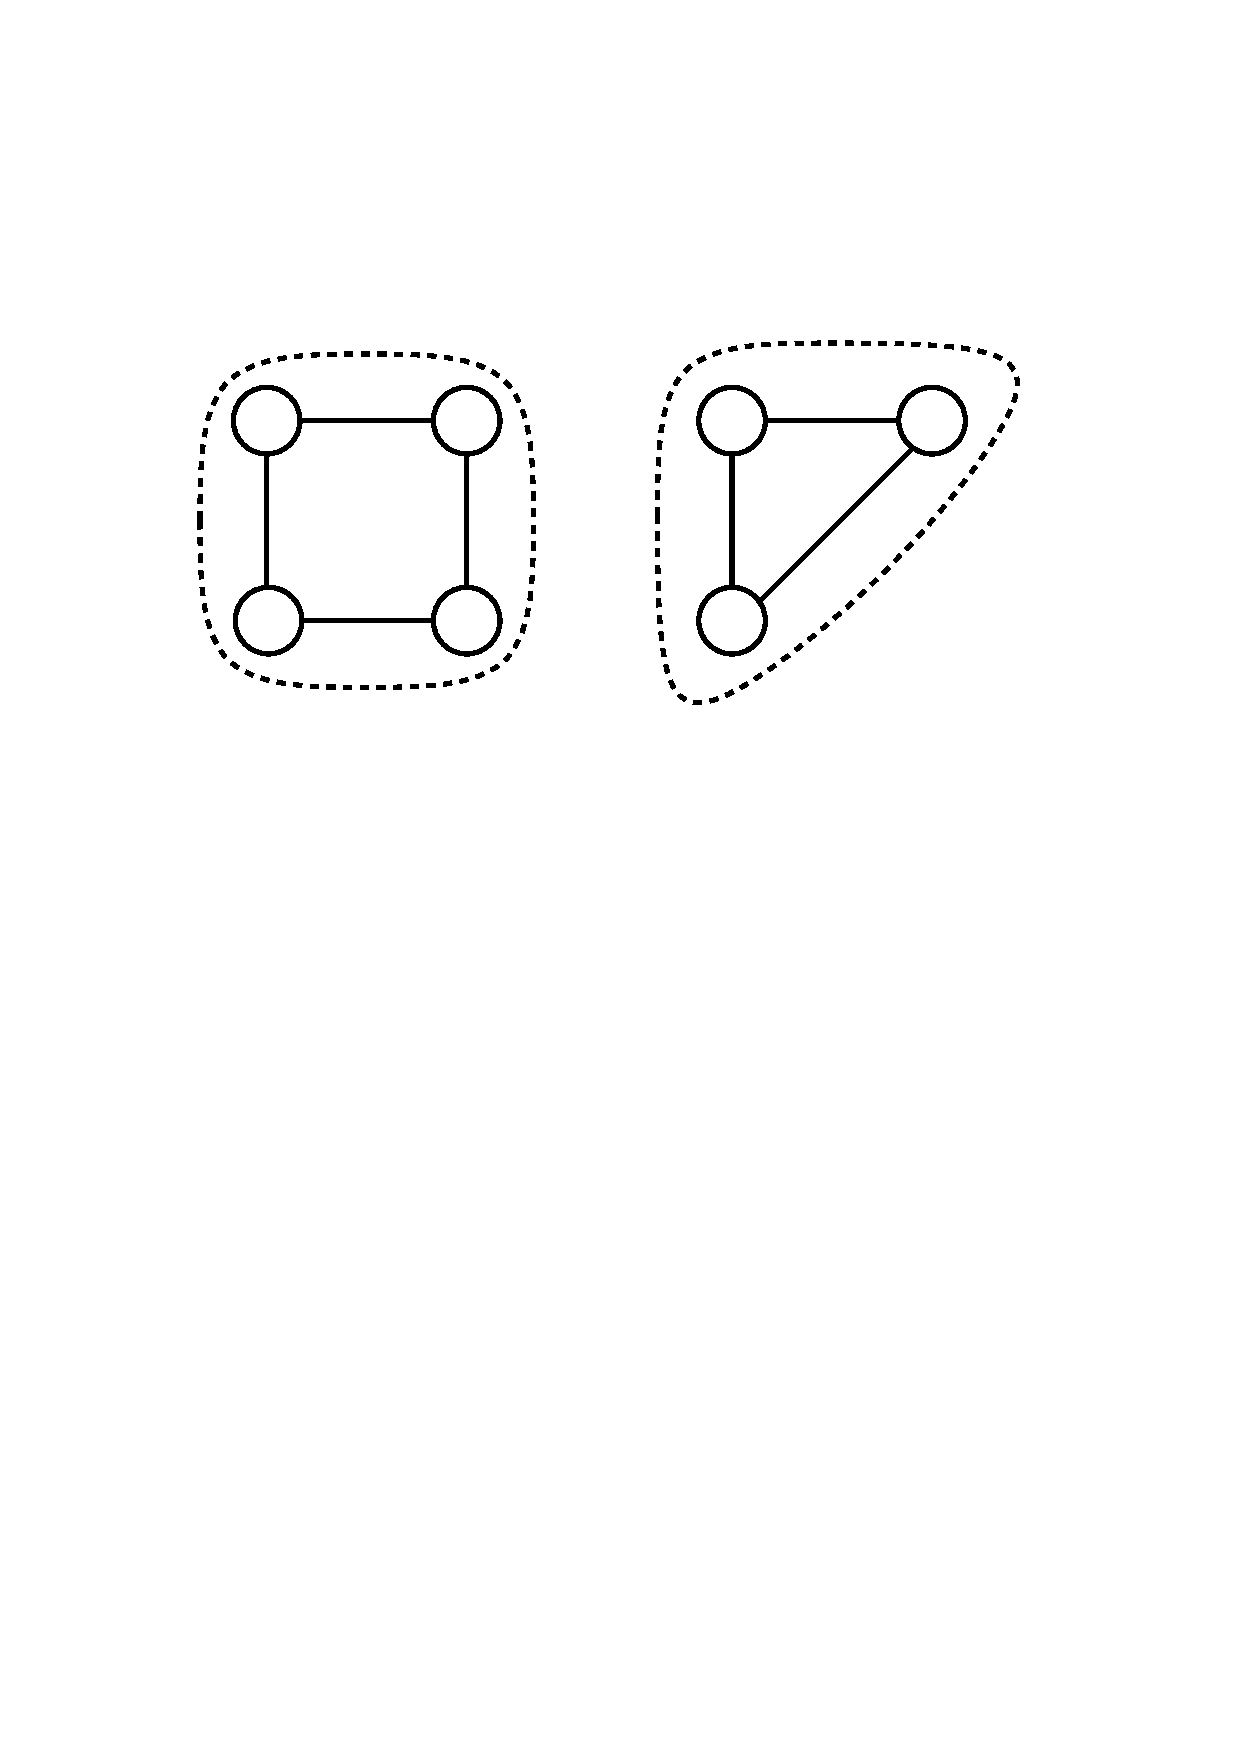
\includegraphics[scale=.5]{01_graph_theory/pics/components.pdf}
	\caption{Graph with 2 components}
\end{figure}
\FloatBarrier

\begin{definition}
\index{graph!connected}
$G$ is \dt{connected} if it has only one component. This means that $\forall v,w: v\operatorname{R} w$.
\end{definition}

\begin{definition}
\index{connected component}
$H\leq G$ is a \dt{connected component} of $G$ if $H$ is connected and $H$
is maximal with regard to the subgraph relation, i.\,e. no vertices or edges can
be added to $H$ so that is still connected: $\nexists H': H < H' \leq G, H'\text{ connected}.$
\end{definition}

\begin{definition}
\index{connectivity}
\index{relation!connectivity relation}
For directed graphs, we define the \dt{connectivity relation} $\operatorname{S}$ as follows:
\begin{align*}
v \operatorname{R} w \text{ ($v$ connected to $w$)} \iff \null
&\text{$\exists$ walk from $v$ to $w$\quad\emph{and}} \\
&\text{$\exists$ walk from $w$ to $v$.}
\end{align*}
Like $\operatorname{R}$, $\operatorname{S}$ is an equivalence relation.
\end{definition}

\begin{definition}
\index{graph!connected!strongly}
$G$ is \dt{strongly connected} $\iff \forall v,w\in V: v \operatorname{S} w$.
\end{definition}

\begin{definition}
\index{connected component!strongly}
$H\leq G$ is a \dt{strongly connected component} of $G$ if $H$ is maximal strongly connected.
\end{definition}

\begin{figure}[htb]
	\centering
	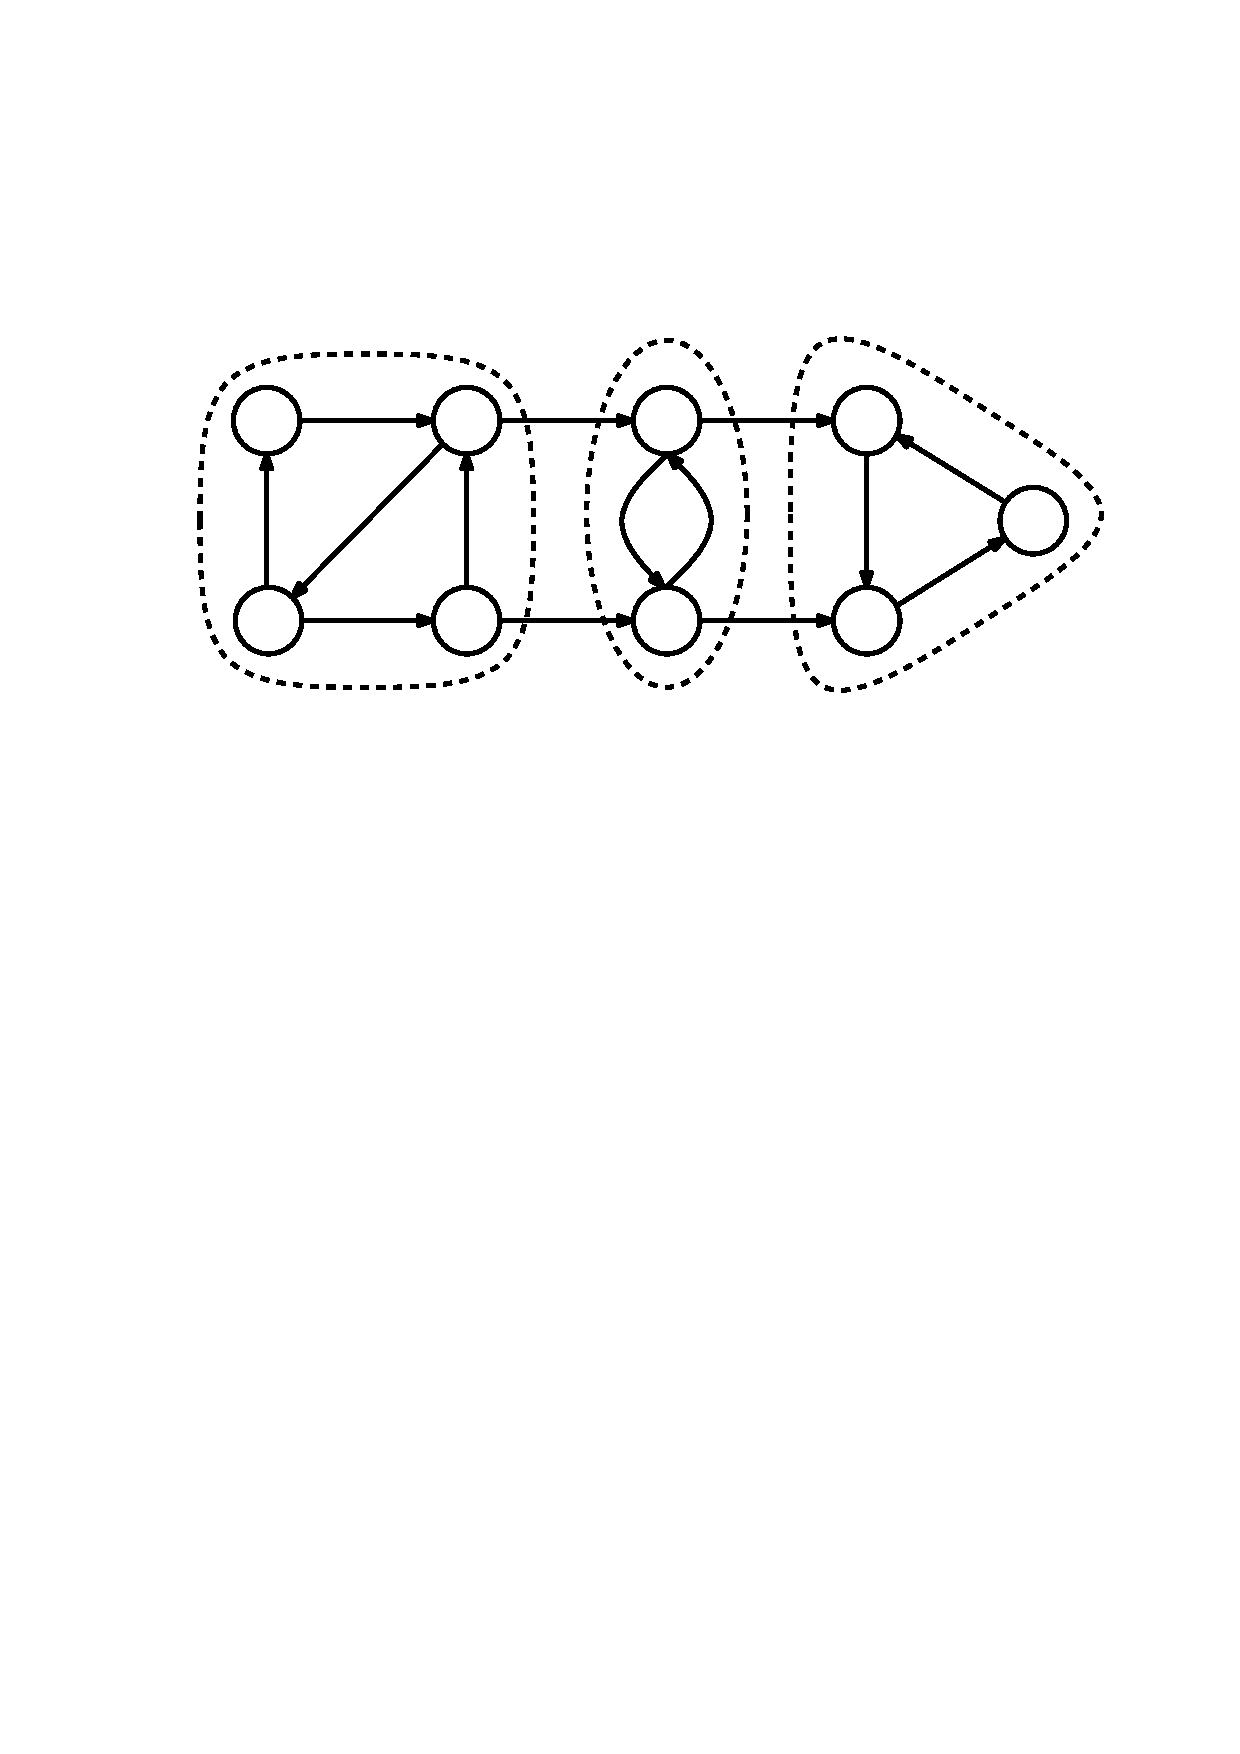
\includegraphics[scale=.5]{01_graph_theory/pics/strongly-connected_component.pdf}
	\caption{graph with 3 strongly connected components}
\end{figure}
\FloatBarrier


%%%  04.10.2013  %%%
%%%  VO 02

\begin{definition}
\strut\lecturedate{2013-10-04}%
\index{shadow}
Let $G$ be a directed graph. The \dt{shadow} $H$ of $G$ is the undirected graph
that results when we ignore edge directions on $G$.
\end{definition}

\begin{definition}
\index{graph!connected!weakly}
$G$ is \dt{weakly connected} if its shadow $H$ is connected.
\end{definition}

\begin{definition}
\def\Gr{\ensuremath{G_\text{R}}}
\def\Vr{\ensuremath{V_\text{R}}}
\def\Er{\ensuremath{E_\text{R}}}
Let $G=(V,E)$ be a directed graph. Let
\[ K_1=\{v_1,\ldots\},K_2,\ldots,K_M \]
be the strongly connected components of $G$. Let $\Gr=(\Vr,\Er)$ with
\begin{align*}
\Vr &= \{K_1,\ldots,K_M\} \\
\Er &= \left\{(K_i,K_j) \mid \exists v\in V(K_i)\,\exists w\in V(K_j): (v,w)\in E\right\}.
\end{align*}
\index{reduction}%
Then we call $\Gr$ the \dt{reduction} of $G$.
\end{definition}

\textbf{Remark.} $G_\text{R}$ is always acyclic.

% strongly connected components
\begin{figure}[htb]
\resizebox{\textwidth}{!}{
\subfigure[directed Graph $G$]
{
	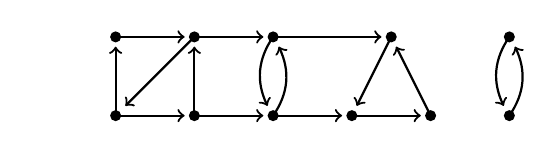
\begin{tikzpicture}
	\node at (0,0) {};
	\node (k1) at (1,0) {};
	\node (k2) at (2,0) {};
	\node (k3) at (2,1) {};
	\node (k4) at (1,1) {};

	\node (k5) at (3,0) {};
	\node (k6) at (3,1) {};

	\node (k7) at (4,0) {};
	\node (k8) at (5,0) {};
	\node (k9) at (4.5,1) {};

	\node (k10) at (6,0) {};
	\node (k11) at (6,1) {};

	\foreach \i in {1,...,11}
	{
		\fill (k\i) circle [radius=2pt];
	};

	\foreach \i / \j in {
	1/2, 2/3, 3/1, 4/3, 1/4,
	7/8, 8/9, 9/7,
	2/5, 3/6,
	5/7,
	6/9}
	{
		\path (k\i.center) edge[->, thick] (k\j);
	};
	\foreach \i / \j in {
	5/6, 6/5,
	10/11, 11/10}
	{
		\path (k\i.center) edge[->, thick, bend right] (k\j);
	};

	\end{tikzpicture}
}
\subfigure[shadow $H$ of Graph $G$]
{
	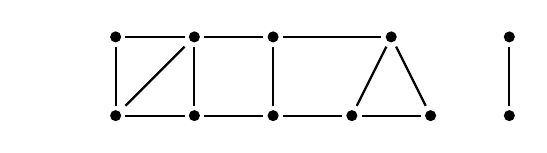
\begin{tikzpicture}
	\node at (0,0) {};
	\node (k1) at (1,0) {};
	\node (k2) at (2,0) {};
	\node (k3) at (2,1) {};
	\node (k4) at (1,1) {};

	\node (k5) at (3,0) {};
	\node (k6) at (3,1) {};

	\node (k7) at (4,0) {};
	\node (k8) at (5,0) {};
	\node (k9) at (4.5,1) {};

	\node (k10) at (6,0) {};
	\node (k11) at (6,1) {};

	\foreach \i in {1,...,11}
	{
		\fill (k\i) circle [radius=2pt];
	};

	\foreach \i / \j in {
	1/2, 2/3, 3/1, 4/3, 1/4,
	7/8, 8/9, 9/7,
	2/5, 3/6,
	5/7,
	6/9,
	5/6, 6/5,
	10/11, 11/10}
	{
		\path (k\i) edge[thick] (k\j);
	};
	\end{tikzpicture}
}}
\resizebox{\textwidth}{!}{
\subfigure[strongly connected components of $G$]
{
	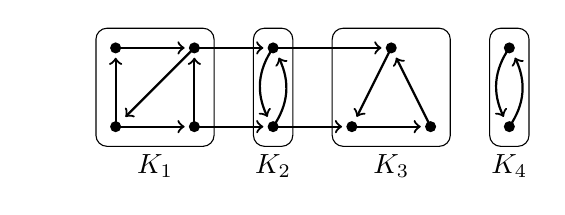
\begin{tikzpicture}
	\node at (0,0) {};
	\node (k1) at (1,0) {};
	\node (k2) at (2,0) {};
	\node (k3) at (2,1) {};
	\node (k4) at (1,1) {};

	\node (k5) at (3,0) {};
	\node (k6) at (3,1) {};

	\node (k7) at (4,0) {};
	\node (k8) at (5,0) {};
	\node (k9) at (4.5,1) {};

	\node (k10) at (6,0) {};
	\node (k11) at (6,1) {};

	\foreach \i in {1,...,11}
	{
		\fill (k\i) circle [radius=2pt];
	};

	\foreach \i / \j in {
	1/2, 2/3, 3/1, 4/3, 1/4,
	7/8, 8/9, 9/7,
	2/5, 3/6,
	5/7,
	6/9}
	{
		\path (k\i.center) edge[->, thick] (k\j);
	};
	\foreach \i / \j in {
	5/6, 6/5,
	10/11, 11/10}
	{
		\path (k\i.center) edge[->, thick, bend right] (k\j);
	};

	\draw[rounded corners] (0.75, -0.25) rectangle (2.25, 1.25);
	\draw[rounded corners] (2.75, -0.25) rectangle (3.25, 1.25);
	\draw[rounded corners] (3.75, -0.25) rectangle (5.25, 1.25);
	\draw[rounded corners] (5.75, -0.25) rectangle (6.25, 1.25);

	\node at (1.5, -0.5) {$K_1$};
	\node at (3.0, -0.5) {$K_2$};
	\node at (4.5, -0.5) {$K_3$};
	\node at (6.0, -0.5) {$K_4$};
	\end{tikzpicture}
}
\subfigure[reduction $G_R$ of Graph $G$]
{
	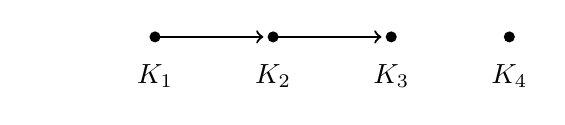
\begin{tikzpicture}
	\node at (0,0) {};
	\node (k1) at (1.5, 0) {};
	\node (k2) at (3.0, 0) {};
	\node (k3) at (4.5, 0) {};
	\node (k4) at (6.0, 0) {};

	\node at (1.5, -0.5) {$K_1$};
	\node at (3.0, -0.5) {$K_2$};
	\node at (4.5, -0.5) {$K_3$};
	\node at (6.0, -0.5) {$K_4$};

	\foreach \i in {1,...,4}
	{
		\fill (k\i) circle [radius=2pt];
	};
	\foreach \i / \j in {1/2, 2/3}
	{
		\path (k\i.center) edge[->, thick] (k\j);
	};
	\end{tikzpicture}
}}
\caption{Graphs}
\end{figure}





\begin{definition}
\index{node base}
Let $G$ be a directed graph. $B$ is a \dt{node base} of $G$ if:
\begin{compactitem}
\item $B\subseteq V$,
\item $\forall v\in V\,\exists w\in B: w \operatorname{S} v$, and
\item $B$ minimal w.\,r.\,t. $\subseteq$.
\end{compactitem}
\end{definition}

\index{node base}
\textbf{Remark.} The node base of $G$ can easily be constructed from a node
base of $G_\text{R}$. Let $\{K_1,\ldots,K_L\}\subseteq V_\text{R}$ be a node
base of $G_\text{R}$. Then
\[ \left\{\{b_1,\ldots,b_l\mid b_i\in V(K_i)\}\right\} \]
is the set of all node bases of $G$.

\index{node base}
$G_\text{R}$ has a single unique node base.

\index{node base}
\textbf{Remark.} The node base of $G_\text{R}$ (or acyclic graphs in general) is
\[ \{K\in V_\text{R}\mid d_{G_\text{R}}^{-}(K) = 0\}. \]




%%%  04.10.2013  %%%
%%%  VO 02
\section{Trees and Forests}

\begin{definition}
\index{forest}
A \dt{forest} is an undirected acyclic graph.
\end{definition}

\begin{definition}
\index{tree}
A \dt{tree} is a connected forest.
\end{definition}

\begin{definition}
\index{tree!rooted}
\index{root}
A \dt{rooted tree} is a tree with one special node designated as the \dt{root}.
\end{definition}

\begin{definition}
\index{tree!plane}
A \dt{plane tree} is a tree embedded into the plane, i.\,e. the order of
children matters. Two trees may be isomorphic, but not equivalent when regarded
as plane trees.
\end{definition}

In Computer Science, trees are often plane and rooted, e.\,g.\ binary search trees.

\begin{definition}
\index{isomorphism}
Two graphs $G$ and $H$ are \dt{isomorphic} ($G \cong H$) if there is a function
\[ \varphi: V(G)\mapsto V(H)\quad\text{$\varphi$ bijective} \]
so that
\[ vw \in E(G) \iff \varphi(v)\varphi(w) \in E(H). \]
\end{definition}

\begin{definition}
\index{leaf}
A \dt{leaf} is a node with degree 1. 
\end{definition}

\textbf{Lemma.}
A non rooted tree $T$ has at least 2 leaves. \\
$|V(T)| \geq 2$

\textbf{Proof.} \TODO{add images} \\
\begin{compactitem}
	\item T of size 2
	\item T of at least 3 nodes, $|V(T)| \geq 3$
	\begin{compactitem}
		\item Case 1:\\
			$|V(T)| = k+1 \Rightarrow |V(T)| = k$ \\
			$\Rightarrow_{imp} T'$ has 2 leaves $\Rightarrow T$ has at least 2 leaves
		\item Case 2: \\
			first node is no leaf, $T'$ and $T''$ each have at least 2 leaves each

	\end{compactitem}
\end{compactitem}


\begin{definition}
\index{bridge}
A \dt{bridge} is an edge whose removal would increase the number of connected components.
\end{definition}


\textbf{Theorem.} The following statements are equivalent:
\begin{compactenum}[(1)]
  \item $T$ is a tree.
  \item $\forall v,w\in V(T)$ $\exists$ unique path from $v$ to $w$
  \item $T$ connected, $|V(T)|=|E(T)|+1$
  \item $T$ minimal connected (every edge is a bridge)
  \item $T$ maximal acyclic
\end{compactenum}
\null\par

\textbf{Proof of 1. $\implies$ 3.} \\
induction on $n = \alpha_0=|V(T)|$

\begin{tabular}{l l}
	$n = 1:$	& trivial, $\cdot$ \\
	$n \rightarrow n+1:$	& Choose leaf $v$ of $T$, $T' = T \backslash \{v\}$ \\
							 &	
	$\begin{array}{ll}
	|V(T')| = |E(T')| + 1 \\
		|V(T')+1 = |E(T')+1 +1 \\
		substitution	& |V(T)| = |V(T')| +1 \\
			& |E(T)| = |E(T')| +1 \\
		|V(T)| = |E(T)| + 1
	\end{array}$
\end{tabular}

\subsection{Spanning Subgraphs}

\begin{definition}
\index{spanning forest}
\index{spanning tree}
Let $G=(V,E)$ be an undirected graph. $F$ is a \dt{spanning forest} of $G$ if and only if:
\begin{compactitem}
  \item $V(F) = V(G)$, $E(F)\subseteq E(G)$,
  \item $F$ is a forest, and
  \item $F$ has the same connected components as $G$.
\end{compactitem}
If $F$ is connected, we call it a \dt{spanning tree}.
\end{definition}

\textbf{Example introducing matrix-tree theorem}\\

% Graph G and all possible spanning trees
\begin{figure}[htb]
\centering
\subfigure
{
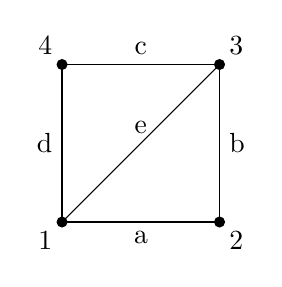
\begin{tikzpicture}[scale=2]

\node (n1) at (0,0) {};
\node (n2) at (1,0) {};
\node (n3) at (1,1) {};
\node (n4) at (0,1) {};

\draw (n1) node[anchor=north east] {$1$};
\draw (n2) node[anchor=north west] {$2$};
\draw (n3) node[anchor=south west] {$3$};
\draw (n4) node[anchor=south east] {$4$};

\foreach \i in {1,...,4}
{
	\fill (n\i) circle [radius=1pt];
};

\foreach \i/ \j/ \label/\position in {1/2/a/below, 2/3/b/right, 
					3/4/c/above, 4/1/d/left, 
					1/3/e/above}
{
	\path (n\i.center) edge node[\position] {\label} (n\j.center);
};
\end{tikzpicture}
}
\subfigure
{
	\begin{tabular}{cccc}
	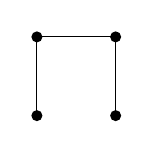
\begin{tikzpicture}

	\node (n1) at (0,0) {};
	\node (n2) at (1,0) {};
	\node (n3) at (1,1) {};
	\node (n4) at (0,1) {};

	\foreach \i in {1,...,4}
	{
		\fill (n\i) circle [radius=2pt];
	};

	\foreach \i / \j in {2/3, 3/4, 4/1}
	{
		\path (n\i.center) edge (n\j.center);
	};
	\end{tikzpicture}
	&
	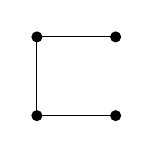
\begin{tikzpicture}

	\node (n1) at (0,0) {};
	\node (n2) at (1,0) {};
	\node (n3) at (1,1) {};
	\node (n4) at (0,1) {};

	\foreach \i in {1,...,4}
	{
		\fill (n\i) circle [radius=2pt];
	};

	\foreach \i / \j in {
	1/2, 
	%2/3, 
	3/4,
	4/1}
	{
		\path (n\i.center) edge (n\j.center);
	};
	\end{tikzpicture}
	&
	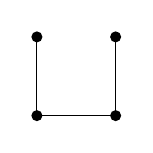
\begin{tikzpicture}

	\node (n1) at (0,0) {};
	\node (n2) at (1,0) {};
	\node (n3) at (1,1) {};
	\node (n4) at (0,1) {};

	\foreach \i in {1,...,4}
	{
		\fill (n\i) circle [radius=2pt];
	};

	\foreach \i / \j in {
	1/2, 
	2/3, 
	%3/4,
	4/1}
	{
		\path (n\i.center) edge (n\j.center);
	};
	\end{tikzpicture}
	&
	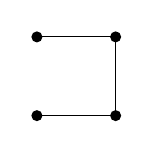
\begin{tikzpicture}

	\node (n1) at (0,0) {};
	\node (n2) at (1,0) {};
	\node (n3) at (1,1) {};
	\node (n4) at (0,1) {};

	\foreach \i in {1,...,4}
	{
		\fill (n\i) circle [radius=2pt];
	};

	\foreach \i / \j in {
	1/2, 
	2/3, 
	3/4}
	%4/1}
	{
		\path (n\i.center) edge (n\j.center);
	};
	\end{tikzpicture}
	\\
	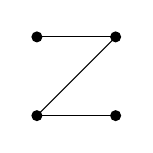
\begin{tikzpicture}

	\node (n1) at (0,0) {};
	\node (n2) at (1,0) {};
	\node (n3) at (1,1) {};
	\node (n4) at (0,1) {};

	\foreach \i in {1,...,4}
	{
		\fill (n\i) circle [radius=2pt];
	};
	\foreach \i / \j in {
	1/2, 
	%2/3, 
	3/4,
	%4/1,
	1/3}
	{
		\path (n\i.center) edge (n\j.center);
	};
	\end{tikzpicture}
	&
	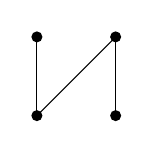
\begin{tikzpicture}

	\node (n1) at (0,0) {};
	\node (n2) at (1,0) {};
	\node (n3) at (1,1) {};
	\node (n4) at (0,1) {};

	\foreach \i in {1,...,4}
	{
		\fill (n\i) circle [radius=2pt];
	};
	\foreach \i / \j in {
	%1/2, 
	2/3, 
	%3/4,
	4/1,
	1/3}
	{
		\path (n\i.center) edge (n\j.center);
	};
	\end{tikzpicture}
	&
	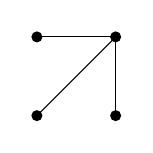
\begin{tikzpicture}

	\node (n1) at (0,0) {};
	\node (n2) at (1,0) {};
	\node (n3) at (1,1) {};
	\node (n4) at (0,1) {};

	\foreach \i in {1,...,4}
	{
		\fill (n\i) circle [radius=2pt];
	};
	\foreach \i / \j in {
	%1/2, 
	2/3, 
	3/4,
	%4/1,
	1/3}
	{
		\path (n\i.center) edge (n\j.center);
	};
	\end{tikzpicture}
	&
	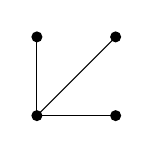
\begin{tikzpicture}

	\node (n1) at (0,0) {};
	\node (n2) at (1,0) {};
	\node (n3) at (1,1) {};
	\node (n4) at (0,1) {};

	\foreach \i in {1,...,4}
	{
		\fill (n\i) circle [radius=2pt];
	};
	\foreach \i / \j in {
	1/2, 
	%2/3, 
	%3/4,
	4/1,
	1/3}
	{
		\path (n\i.center) edge (n\j.center);
	};
	\end{tikzpicture}

	\end{tabular}
}
\caption{Graph $G$ and all its spanning trees}
\end{figure}





\begin{equation*}
\begin{array}{ll}
	\tilde A = \begin{pmatrix}
		0 & a & d & e \\
		a & 0 & 0 & b \\
		d & 0 & 0 & c \\
		e & b & c & 0 
	\end{pmatrix}
	&
	\tilde D = \begin{pmatrix}
		a+d+e \\
		& a+b \\
		& & c+d \\
		& & & b+c+e \\
	\end{pmatrix}
\end{array} 
\end{equation*}
\begin{equation*}
	\tilde D - \tilde A = \begin{pmatrix}
		\tikzmark{topA}a+\tikzmark{topA2}d+e & -a & -d & -\tikzmark{topB}e \\
		 -a & a+b & 0 & -b \\
		-d & 0 & c+d & -c \\
		-\tikzmark{botA}e & -b & -c & b+c+e \\
	\end{pmatrix}
\end{equation*}
\DrawLineHorizontal[red, thick, opacity=0.5]{topA}{topB}
\DrawLine[red, thick, opacity=0.5]{topA2}{botA}

\begin{equation*}
\begin{array}{ll}
\begin{vmatrix}
	a+b & 0 & -b \\
	0 & c+d & -c \\
	-b & -c & b+c+e
\end{vmatrix} 
& = (a+b)(c+d)(b+c+e)-b^2(c+d)-c^2(a+b) \\
& = bcd + abc+ abd +acd + ace + ade + bce + bde \\
& \text{every term represents a spanning tree}
\end{array}
\end{equation*}

if we set $a=b=c=d=1$ then

\begin{itemize}
	\item $\tilde A \rightarrow A$
	\item $\tilde D \rightarrow D = 
		\begin{pmatrix}3 \\ & 2 \\ & & 2 \\ & & & 3 \\ \end{pmatrix}$
	\item $\det{(D-A)'} = 8$
\end{itemize}

\textbf{Theorem (Kirchhoff's Matrix-Tree Theorem).}
Let
\begin{align*}
G &&& \text{undirected connected graph,} \\
A &&& \text{adjacency matrix,} \\
\operatorname{diag}(d(v_1),\ldots,d(v_n)) = D &&& \text{degree matrix,} \\
(D-A)' &&& \text{$D-A$ with one row and one column removed.}
\end{align*}
Then $|\det{(D-A)'}|$ is the number of spanning trees of $G$.

\textbf{Remark.} If $G$ is not connected, the number of spanning trees can be
found for each connected component. Multiply results to get the number
of possible combinations.


% Minimal or Maximal Spanning Tree
% sub problem
% Minimal or maximal Spanning Trees
\begin{figure}[htb]
\centering
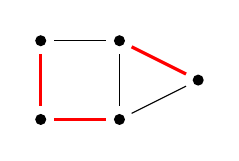
\begin{tikzpicture}[every node/.style = {circle}]

\node (a) at (0,0) {};
\node (b) at (1,0) {};
\node (c) at (2,0.5) {};
\node (d) at (1,1) {};
\node (e) at (0,1) {};
\foreach \node in {a,...,e}
{
	\fill (\node) circle [radius=2pt];
};

\draw[red,very thick] (a) -- (b);
\draw[red,very thick] (a) -- (e);
\draw[red,very thick] (c) -- (d);
%\draw (a) -- (b);
%\draw (a) -- (e);
\draw (b) -- (c);
\draw (b) -- (d);
%\draw (c) -- (d);
\draw (d) -- (e);
\end{tikzpicture}
\caption{Graph $G$ and its maximal spanning forest}
\end{figure}





% Proof: F_1, F_2 \sub E
% Observe:
% connecting the trees of a forest with edge e
\begin{figure}[htb]
\centering
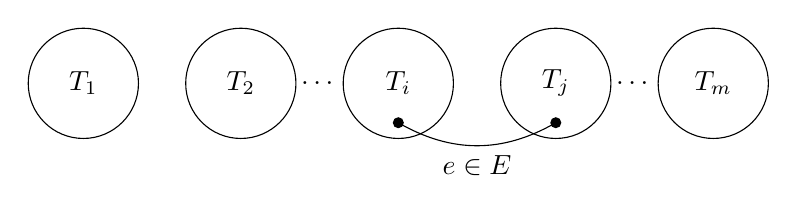
\begin{tikzpicture}
\node[] (T1) at (0,0) {$T_1$};
\node[] (T2) at (2,0) {$T_2$};
\node[] (T_dots1) at (3,0) {\ldots};
\node[] (Ti) at (4,0) {$T_i$};
\node[] (Tj) at (6,0) {$T_j$};
\node[] (T_dots2) at (7,0) {\ldots};
\node[] (Tm) at (8,0) {$T_m$};
\node[] (Ti_e) at (4,-0.5) {};
\node (Tj_e) at (6,-0.5) {};

\draw \foreach \n in {T1, T2, Ti,Tj,Tm}
{
	(\n) circle (0.7)
};

\fill (Ti_e) circle [radius=2pt];
\fill (Tj_e) circle [radius=2pt];

\path (Ti_e.center) edge [bend right] node[below] {$e \in E$} (Tj_e.center) ;

\end{tikzpicture}
\caption{Forest $F_2$ and its trees}
\end{figure}



\missingdate{2013-10-10}
\missingdate{2013-10-11}


%!TEX root = ../main.tex

\section{Matroids and Greedy Algorithms}

\textit{Kruskal} and \textit{Prim} are greedy algorithm for maximalization/minimalization.

\textbf{Claim:} In general, greedy strategies fail, but for \dt{matroid}s they always work.\\

\textbf{Kruskal:} edges sorted according to weight, always take the next best one with the restriction that it must not create a cycle.

\begin{definition}
\index{independence system}
$(E, S)$ is an \dt{independence system} if $S \subseteq 2^E$, $S$ closed under set-inclusion i.e. $A\in S$, $B \subseteq A \Rightarrow B\in S$.\\
$S$ is the set of independent sets.
\end{definition}

\textbf{Optimization Problem}:
\[ (E, S), w: E \rightarrow \mathbb{R}, A\subseteq E: w(A) = \sum_{e\in A} w(e)\]
Search for $A$ s.t.
\[ w(A) \text{ maximal(/minimal)}, A\in S, A \text{ max w.r.t. } \subseteq\]

\textbf{Example:} $(E, S)$, $E$ edge set, $S$ is set of forests.\\\\
\textbf{GREEDY} $E, S, w, T$
\begin{enumerate}
	\item{sort elements of $E$ according to weight: $E=\{e_1, ... e_k|w(e_1)\le w(e_2)\le...\}$}
	\item{$T=\emptyset$}
	\item{for $K=1...m$: if $T\cup\{e_k\} \in S $ then $T:= T\cup\{e_k\}$}
\end{enumerate}

\begin{definition}
	\index{independence system}
	\index{matroid}
	$M=(E, S)$ \dt{independence system} \dt{matroid} if
	\[
	A, B \in S~~s.t.~~|B|=|A|+1\Rightarrow\exists v\in B\setminus A \text{ with } A\cup\{v\}\in S
	\]
\end{definition}

\textbf{Remark:} matroid property holds in general for $A,B \in S~~s.t.~~|A|<|B|$ as well\\

\begin{definition}
	\index{independence system!basis}
	\index{matroid!rank}
	$A\in S$ \dt{basis} of $M \Leftrightarrow A$ max (w.r.t. set inclusion $\subseteq$) independent set
	\[
	A, B \text{ basis of } M \Rightarrow |A| = |B| = r(M)
	\]
	$r(M)$... \dt{rank} of the matroid
\end{definition}

\textbf{Theorem.}
\[G=(V,E) \text{ graph, }S=\{F\subseteq E | F \text{ forest}\} \Rightarrow (E,S) \text{ is a matroid}\]
\textbf{Proof:}
\begin{compactenum}[(1)]
	\item{$F_1, F_2 \in E,~F_2\in S,~F_1\subseteq F_2\Rightarrow F_1\subseteq S$}
	\item{$F_1, F_2\in S, ~|F_2| = |F_1| + 1$}
	\item{$F_1$} has $m$ connected components $T_i=(V_i, A_i),~i=1..m$
	\item{Observation: \\
	$V=V_1\cup V_2\cup ... \cup V_m$\\
	$F_1 = A_1\cup A_2\cup ... \cup A_m$\\
	$|A_i|=|V_i|+1$}
	\item{\TODO{Sketch from the notes}}
	\item{Note: $F_2$ is forest $\Rightarrow$ there are at most $|V_i|-1$ edges in $E_2$ which connect $v\in V_i$ $|F_2| > |F_1| \Rightarrow \exists v,w $ in different components, s.t. $(v,w)$ is an edge of $F_2$ connecting these two components $\Rightarrow F_1\cup\{(v,w)\}$ is still a forest}
\end{compactenum}


\TODO{Please someone check this, my notes are kind of sloppy at this point, it was at the end of a lecture :P}
\textbf{Example:} $E=\{a_1, a_2, ... a_n\}$, $a_1, ... a_n \in \mathbb{R}^m$,
$S = \{A\subseteq E | A=\emptyset \text{ or A linear independent}\}$\\
\[A \text{ basis of } S \Leftrightarrow A \text{ basis }
\]
\[
	[E] \text{ is a vector space}
\]
\[
	\text{rank of M: } r(M) = dim[E],~A,B\in S,~|A|+1=|B|\Rightarrow \exists x\in B \text{ s.t. } A\cup \{x\}\in S
\]

\textbf{Theorem: } Let $M=(E, S)$ be a matroid with weight function $w:E\rightarrow \mathbb{R}$\\
$\Rightarrow$ \textbf{GREEDY} solves $A$ max (w.r.t. $\subseteq$) s.t. $w(A)$ min/max correct. (\textbf{GREEDY} computes basis with min/max weight)\\\\
\textbf{Proof: } $A=\{a_1, a_2, ... a_r\}$ set after running \textbf{GREEDY}
\begin{compactenum}
	\item{
		\begin{compactenum}[(a)]
			\item{$A$ basis: $A\in S$ by construction\\
			Assume $A$ not minimal: $\exists e \in E~~s.t.~~A\cup\{e\}\in S$\\ \textbf{CONTRADICTION}
			}
			\item{$w(a_1)\le w(a_2) \le ... w(a_r)$ (elements are sorted) $\checkmark$}
			\item{$w(A)$ minimal}
		\end{compactenum}
	\item{Assume $\exists B = \{b_1, b_2, ... b_3\}$ basis, $w(B) < w(A),~ w(b_1\le w(a_1, ... w(b_3\le w(a_r)$\\
	$i=min\{j | w(b_j)\le w(a_j)\}$}\\
	$A_{i-1}=\{a_a, a_2, ... a_{i-1}\}$ status of $A$ after $m\le i-1$ iterations of greedy\\
	$B_i = \{b_1, b_2, ... b_{i-1}, b_i\}$\\
	$\Rightarrow |B_i| = |A_{i-1}|+1$
	}
	\item{Apply matroid condition:\\
	$b_j = B_i \setminus A_{i-1}~~s.t.~~A_{i-1}\cup \{b_j\}\in S$}
	\item{But:\\
	$w(b_j)\le w_(b_i) < w(a_i) \Rightarrow \forall x \in B_i : w(x) < w(a)$}
	\item{Thats not how greedy works, greedy would have taken $b_j)$ already\\
	$\Rightarrow$ \textbf{CONTRADICTION}}
\end{compactenum}

\textbf{Theorem: } $M(E, S)$ independence system\\
Assume: \textbf{GREEDY} solves the optimization problem \"A max s.t. $w(A)$ min/max\" correctly for all weight functions $w$\\
$\Rightarrow$ M is a matroid.\\\\
\textbf{Proof: } Assume $M$ not a Matroid
\begin{compactenum}
	\item{
	$\exists A, B, \in S: |B| = |A| + 1 \land \forall x \in B \setminus A: A\cup \{x\} \notin S$\\
	Set $w(e) = \begin{cases} 	|A| + 2 & \text{ if } e\in A\\
								|A| + 1 & \text{ if } e \in B\setminus A\\
								0 & else
				\end{cases} $
	}
	\item{
	$w(A) = |A| * (|A| + 2) < (|A| + 1)^2 < w(B)$
	}
	\item{
	$\Rightarrow~A$ not solution of the optimisation Problem, $w(A)$ not maximal
	}
\end{compactenum}

\section{Weighted Graphs and Algorithms}
\TODO{Missing parts from second week}

\subsection{Maximal Flows}

\def\dminus{\ensuremath{d^{-}}}
\def\dplus{\ensuremath{d^{+}}}
\def\real{\mathbb{R}}
\def\natural{\mathbb{N}}
\def\Gammaplus{\ensuremath{\Gamma^{+}}}
\def\Gammaminus{\ensuremath{\Gamma^{-}}}

\begin{definition}
\index{flow network}
Let $G=(V,E,w)$ be a directed network with
\begin{compactitem}
\item a weight function $w: E\mapsto \real_0^{+}$,
\item a source $s: \dminus(s) = 0$ and
\item a sink $t: \dplus(t) = 0$.
\end{compactitem}
Then $(V, E, w, s, t)$ is a \dt{flow network}.
\end{definition}

\begin{definition}
\index{flow}
$\phi: E\mapsto \real$ is a \dt{flow} on $G$ if
\begin{align*}
  &\forall e\in E: 0 ≤ \phi(e) ≤ w(e)
     &&\text{feasability condition} \\
  &\forall x\in V\setminus\{s,t\}:
     \underbrace{\sum_{y\in \Gammaminus(x)} \phi(yx)}_{\text{in-flow}} =
     \underbrace{\sum_{y\in \Gammaplus(x)} \phi(xy)}_{\text{out-flow}}
     &&\text{flow conservation condition} \\
\end{align*}
\end{definition}

\begin{definition}
The \dt{size} or \dt{valuation} $v(\phi)$ of $\phi$ is
\[
  v(\phi) = \sum_{y\in \Gammaplus(s)} \phi(sy).
\]
\end{definition}

\TODO{Lemma+Proof out-flow of source = in-flow of sink}

% new content

\begin{definition}
\index{cut!of a flow network}
\strut\lecturedate{2013-10-17}
A partition $V=S \cup T$ ($S\cap T=\varnothing$) such that $s \in S, t \in T$
is called a \dt{cut} of $G$.
\end{definition}

\begin{definition}
\index{capacity!of a cut}
The \dt{capacity} $c(S,T)$ of a cut is given by
\[ c(S,T) = \sum_{x\in S, y\in T} w(xy). \]
\end{definition}

A cut $(S,T)$ is minimal if all cuts $(S',T')$ satisfy $c(S', T') \geq c(S,T)$.

\Lemma. Let $G$ flow network, $\phi$ flow on $G$, $(S,T)$ cut of G. Then
\[
v(\phi) = \underbrace{\sum_{x\in S, y\in T} \phi(xy)}_{\text{flow forward}}
        - \underbrace{\sum_{x\in T, y\in S} \phi(xy)}_{\text{flow backwards}}
\leq c(S,T).
\]
In particular,
\[
  \max_{\text{flow $\phi$}} v(\phi)\leq \min_{\text{cut $(S,T)$}} c(S,T).
\]

\Proof.
\[
    v(\phi) = \sum_{v\in S} \left(
        \sum_{x\in \Gamma^+(v)} \phi(vx)
      - \sum_{y\in \Gamma^-(v)} \phi(yv)
    \right)
\]

For each vertex, we count flow on outgoing edges positive and flow on
incoming edges negative. We have the following cases:
\begin{itemize}
  \item Flow with both endpoints in $S$; outgoing and ingoing cancel each other
  \item Flow with starting point in $S$ and end point in $T$, counted positive
  \item Flow with starting point in $T$ and end point in $S$, counted negative
\end{itemize}

\begin{figure}[htb]
  \centering
  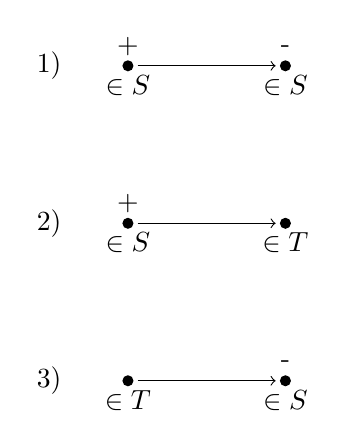
\begin{tikzpicture}
    \node (a0) at (0,0) {1)};
    \node (a1) at (1,0) {};
    \node (a2) at (3,0) {};
    \node (b0) at (0,-2) {2)};
    \node (b1) at (1,-2) {};
    \node (b2) at (3,-2) {};
    \node (c0) at (0,-4) {3)};
    \node (c1) at (1,-4) {};
    \node (c2) at (3,-4) {};
    
    \node at (1,0.25) {+};
    \node at (3,0.25) {-};
    \node at (1,-2 +0.25) {+};
    \node at (3,-4 +0.25) {-};
  
    \node at (1,-0.25) {$\in S$};
    \node at (3,-0.25) {$\in S$};
    \node at (1,-2.25) {$\in S$};
    \node at (3,-2.25) {$\in T$};
    \node at (1,-4.25) {$\in T$};
    \node at (3,-4.25) {$\in S$};
  
    \def\numone{1}
    \def\numtwo{2}
    \foreach \node in {a,b,c} 
    {
      \fill (\node\numone) circle(2pt);
      \fill (\node\numtwo) circle(2pt);
      \path (\node\numone) edge[->] (\node\numtwo);
    };
    
  \end{tikzpicture}
  \caption{3 possible cases}
\end{figure}


Thus, we can rewrite $v(\phi)$:
\[
    v(\phi) = \sum_{x\in S, y\in T} \phi(xy)
            - \sum_{x\in T, y\in S} \phi(xy)
\]
Observe that in the first sum, all $\phi (xy) \leq w(xy)$. The second sum is
nonnegative: $0 \leq \phi (xy) \leq c(S,T)$.

Thus
\[
    v(\phi) \leq c(S,T).
\]

\begin{definition}
\index{augmenting path}
A path $P: s\rightarrow t$ (ignoring edge direction) is said to be an \dt{augmenting
path} with respect to a flow $\phi$ if $\phi(e) < w(e)$ on every forward edge
of $P$ and $\phi(e) > 0$ on every backward edge.
\end{definition}

\textbf{Theorem.}
Let $G$ flow network, $\phi$ flow on $G$. Then 
\[v(\phi)\text{ maximal} \iff \nexists\text{ augmenting path (w.r.t. $\phi$)}.\]

\ProofForward.
Suppose there is an augmenting path $P$. Then we choose
\begin{alignat*}{3}
    \delta' &= \min_{e \in P,\text{ forward}} w(e) - \phi(e) &\null> 0 \\
    \delta'' &= \min_{e\in P,\text{ backward}} \phi(e) &\null> 0 \\
    \delta &= \min(\delta', \delta'') &> 0
\end{alignat*}

Define
\[
    \tilde\phi := \begin{cases}
        \phi(e) + \delta &\text{if $e$ forward edge of $P$} \\
        \phi(e) - \delta &\text{if $e$ backward edge of $P$} \\
        \phi(e) &\text{otherwise}.
    \end{cases}
\]

$\tilde\phi$ is a flow on $G$.

Because we take the minimum of all the flows $\delta$, $\tilde\phi$ does not become negative on backward edges.

Because we increase the flow on the augmenting path by $\delta$,
\[
    v(\tilde\phi) = v(\phi) + \delta > v(\phi).
\]

\ProofBackward.
Assume there is no augmenting path. Let
\[
    S = \{v\in V \mid \exists\;\text{augmenting path $s\rightarrow v$}\}.
\]
There is no augmenting path $s\rightarrow t$, thus $t \notin S$.
Thus $(S, T = V\setminus S)$ is a cut.
Each edge $xy$ with $x\in S, y\in T$ must be saturated: otherwise it would be possible to find an augmenting path.

\begin{figure}[htb]
  \centering
  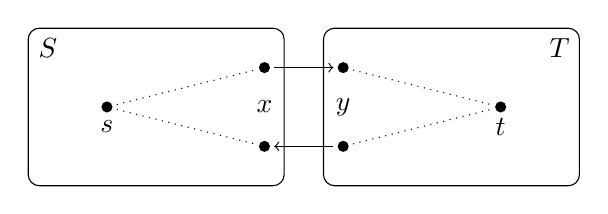
\begin{tikzpicture}
    \node (s) at (2,2) {};
    \node (x1) at (4,2.5) {};
    \node (x2) at (4,1.5) {};
    \node (y1) at (5,2.5) {};
    \node (y2) at (5,1.5) {};
    \node (t) at (7,2) {};
  
    \node at (2,1.75) {$s$};
    \node at (7,1.75) {$t$};
    \node at (4,2) {$x$};
    \node at (5,2) {$y$};
  
    \foreach \node in {s,x1,x2,y1,y2,t}
    {
      \fill (\node) circle(2pt);
    };
    \path (x1) edge[->] (y1);
    \path (y2) edge[->] (x2);

    \path[dotted] (s) edge (x1);
    \path[dotted] (s) edge (x2);
    \path[dotted] (y1) edge (t);
    \path[dotted] (y2) edge (t);

    \node (S) at (1.25,2.75) {$S$};
    \node (T) at (7.75,2.75) {$T$};
    \draw[rounded corners] (1,1) rectangle (4.25,3);
    \draw[rounded corners] (4.75,1) rectangle (8,3);
  \end{tikzpicture}
  \caption{Proof augmented path}
\end{figure}



Each edge $xy$ with $x\in T, y\in S$ must be void ($\phi(xy) = 0$). Thus
\[
    v(\phi) = c(S,T) - 0.
\]

Therefore $\phi$ must be maximal.

\textbf{Theorem.} If $G$ is a flow network such that $\forall e\in E': w(e)\in
\mathbb{N}$, a maximal flow exists.

\textbf{Proof.} $ \phi_{0}(e) \equiv 0$, if $\phi_{0}$ not max $\implies \exists$ augmenting path with $\delta \in \mathbb{N^{+}}$

Construct $\phi_1$ according to previous proof ($\tilde\phi$). We know that $v(\phi_1) ≥ 1$. Now we iterate and get $\phi_2, v(\phi_2) ≥ 2$,~\ldots After finitely many steps, we reach a flow $\phi_{\text{max}}$ where we cannot find an augmenting path anymore.

\textbf{Corollary.} If $G$ is a flow network with a weight function $w: E\mapsto \mathbb{Q}$, this implies $\exists\;\text{maximal flow}$.

\textbf{Remark.}
If weights are real, it can also be shown that a maximal flow exists (but you need a different proof strategy).

\textbf{Theorem (Max-flow/min-cut theorem).}
Let $G$ be a flow network $\implies \exists$ max. flow and $v(\phi_{\text{max}})= \min_{(S,T) cut} c(S,T)$

% slides: Algorithm of Ford-Fulkerson

\section{Special Graph Classes}

\subsection{Eulerian Graphs}

\begin{definition}
An \dt{Eulerian trail}, which can be open or closed, is a trail where no edge is repeated and every edge is used. In a closed trail or \dt{Eulerian tour}, start = end.
\end{definition}

\begin{definition}
A graph is called \dt{Eulerian} if there is an Eulerian tour.
\end{definition}

\textbf{Theorem.}
Let $G=(V,E)$ be an undirected, connected multigraph. Then
\[
  G\text{ is Eulerian} \iff \forall x\in V: d(x)\text{ even}.
\]

There is an \emph{open} Eulerian trail $\iff$ exactly two vertices have odd degree.

\textbf{Proof.}
% "<==" direction
Proof by induction on $\alpha_1(G) =: m$.

$m = 0$: Trivial, only one vertex.

$m ≥ 1$: construct a tour $W$. You can always find a tour because degrees are even, thus every time you enter a vertex you can certainly find an edge where you can leave it.

Two cases:
a) $W$ is an Eulerian tour
b) $W$ is not an Eulerian tour

Then remove $W$, resulting in a graph $G'$ with connected components $G'_1$,~\ldots Then
\[
    \forall x\in V(G'_{i}): d_{G'}(x)\text{ is still even}
\]

Since all $G'_{i}$ are smaller than $G$, we can apply the induction hypothesis. This means $G'_{i}$ must be Eulerian (with Eulerian tours $W_{i}$).

$\forall i: W_i$ and $W$ have common vertex. Thus you can construct an Eulerian tour for the whole graph.

% Slides: Eulerian tour (started at 09:57... :)

% "==>" direction

Walk on an Eulerian tour.



% Discrete Mathematics Lecture Notes 2013-10-18

\subsection*{Hamiltonian Graphs}
\lecturedate[\baselineskip]{2013-10-18}

\begin{definition}
In a \dt{Hamiltonian cycle}, each vertex is visited exactly once (except start/end).
$\text{$G$ is \dt{Hamiltonian}} \iff \exists\;\text{Hamiltonian cycle}.$
\end{definition}

Finding a Hamiltonian cycle in a graph is an NP-complete problem.

\begin{definition}
Let $G=(V,E)$ be a graph.
\[
%\forall v,w\in V :  \rightarrow\text{add $vw$ to $E$}\leadsto \tilde E
\tilde E = E\cup \{vw \mid v,w\in V,\; d(v)+d(w) ≥ |V|\}
\]
Then $[G] = (V,\tilde E)$ is called the \dt{closure} of $G$.
\end{definition}

\Theorem.  $G\text{ Hamiltonian} \iff [G]\text{ Hamiltonian}.$

\ProofForward.
Trivial.

\ProofBackward.
Choose
\begin{gather*}
  v,w\in V: vw \not\in E(G),\;d(v)+d(w) ≥ |V| \\
  H=(V,E\cup \{vw\})
\end{gather*}
Assume $H$ is Hamiltonian and $G$ is not.
This means that $\exists\;\text{Hamiltonian cycle in $H$}$ and it must contain $vw$.
In $H$ containing $vw$, say
\[ v=x_1,x_2,x_3,\ldots,x_n=w,x_1 \qquad(n=|V|)\]
Let
\begin{align*}
    X &=\{x_i \mid x_{i-1}\in \Gamma_G(w), 3 ≤ i ≤ n-1 \}\quad\text{and} \\
    Y &=\{x_i \mid x_i\in \Gamma_G(v), 3 ≤ i ≤ n-1 \}.
\end{align*}

\path{v, x_2, x_3, \ldots, x_{n-1}, w} is a path in $G$.

$v \not\in \Gamma_G(w) \implies |X| = d_G(w) - 1$
because exactly one neighbour is excluded, all the others are counted. $x_1= v$ is not a neighbour by our assumption.

$x_2, x_3, \ldots x_{n-2}$ there is one neighbour $x_{n-1}$ of $w$ which is not counted. 

Analogously,
$|Y| = d_G(v) - 1$.

Thus $|X| + |Y| \geq n-2$.

Therefore, $\exists\,i: 3 ≤ i ≤ n-1$ such that
$x_{i-1}\in \Gamma_G(w), x_i\in\Gamma_G(v)$, because we iterate over $n-3$ values.

$\implies \path{v=x_1, x_i, x_{i+1}, \ldots, x_{n-1}, w=x_n, x_{i-1}, x_{i-2}, \ldots, x_2, v=x_1}$

But this is a Hamiltonian cycle in $G$ (contradiction).

If $H$ is not Hamiltonian, you could add other edges, but by the same argument, this will not lead to a Hamiltonian graph.

\textbf{Corollary 1.}
Let $G=(V,E), |V| ≥ 3$, such that
\[
    \forall v,w\in V: vw\not\in E\implies d(v) + d(w) \geq |V|.
\]
Then $G$ is Hamiltonian.

\textbf{Corollary 2.}
If 
$\forall v \in V : d(v) \geq \frac{n}{2}$,
then $G$ is Hamiltonian.

The generalization of this problem, where you want to find an optimal Hamiltonian cycle in a weighted graph, is known as the \emph{Traveling Salesman Problem}.


\subsection*{Planar Graphs}

\begin{definition}
A graph $G$ is \dt{planar} if there is an isomorphic graph $H$ embedded in the plane ($= \mathbb{R}^2$) such that no two edges intersect.
\end{definition}

\textbf{Examples for planar and non-planar Graphs}
\begin{figure}[htb]
  \centering
  \subfloat[$K_3$, planar]{
    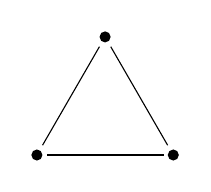
\begin{tikzpicture}
      \fullyConnectedGraph{90,-30,180+30}{1cm}
    \end{tikzpicture}
  }
  \subfloat[$K_4$, planar]{
    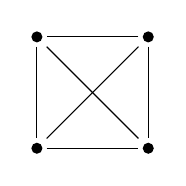
\begin{tikzpicture}
      \fullyConnectedGraph{90-45, 90+45, -90-45, -90+45}{1cm}
    \end{tikzpicture}
  }
  \subfloat[$K_4$, planar, alternative]{
    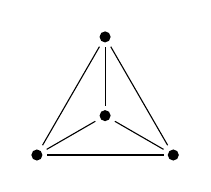
\begin{tikzpicture}
      \fullyConnectedGraph{90,-30,180+30}{1cm}
      \node (n0) at (0,0) {};
      \fill (n0) circle(2pt);
      \foreach \i in {1,...,\the\value{nodecount}} {
	\path (n0) edge (n\i);
      };
    \end{tikzpicture}
  }
  \subfloat[$K_5$, nonplanar]{
    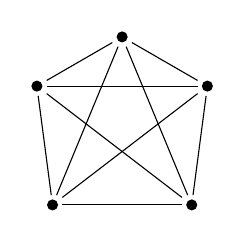
\begin{tikzpicture}
      \fullyConnectedGraph{90, 30, 180-30, -90-45, -90+45}{1.25cm}
    \end{tikzpicture}
  }
  \subfloat[$K_{3,3}$, nonplanar, bipartite]{
    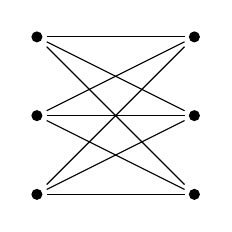
\begin{tikzpicture} % pipartite graph K_{3,3}
      \foreach \i in {1,...,3} {
	\node (n1\i) at (0,\i) {};
	\node (n2\i) at (2,\i) {};
	\fill (n1\i) circle(2pt);
	\fill (n2\i) circle(2pt);
      };
      \foreach \i in {1,...,3}
      {
	\foreach \j in {1,...,3}
	{
	  \path (n1\i) edge (n2\j);
	};
      };
    \end{tikzpicture}
  }
  \caption{Examples for (non-)planar Graphs}
\end{figure}


% triangle (planar)
% square with diagonals (planar) ≅ square with second diagonal non-intersecting
% K_5 (non-planar)
% bipartite graph K_{3,3} (non-planar)

$K_5$ is the smallest non-planar complete graph, $K_{3,3}$ is the smallest non-planar complete bipartite graph.

\begin{definition}
The edges of the graph (which have to be \emph{Jordan curves}) divide the plane into regions. These are the \dt{faces} of the planar graph.
\end{definition}

% Faces of K_4 - Inner: I, II, III, Outer: IV
\begin{figure}[htb] % K4 with the 4 faces labeled
  \centering
  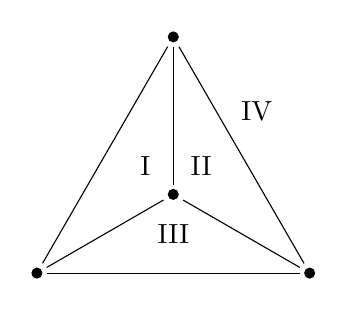
\begin{tikzpicture}
    \fullyConnectedGraph{90,-30,180+30}{2cm}
    \node (n0) at (0,0) {};
    \fill (n0) circle(2pt);
    \foreach \i in {1,...,\the\value{nodecount}} {
      \path (n0) edge (n\i);
    };
    \node at (90+45:0.5cm) {I};
    \node at (45:0.5cm) {II};
    \node at (-90:0.5cm) {III};
    \node at (45:1.5cm) {IV};
  \end{tikzpicture}
  \caption{Faces of $K_4$}
\end{figure}




In the $K_4$, we get
\begin{align*}
    \alpha_0 &= 4 \\
    \alpha_1 &= 6 \\
    \alpha_2 &= 4\quad\text{number of faces}
\end{align*}

\begin{definition}
$H$ is a \dt{subdivision} of $G$ if $H$ is obtained by replacing every edge of $G$ by a path.
\end{definition}
% graph with 4 v and its graph with pathes

\begin{figure}[htb] % K4 and its subdivision
  \centering
  \subfloat[Graph $G$] {
    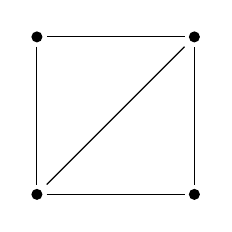
\begin{tikzpicture}
      \node (n1) at (0,0) {};
      \node (n2) at (2,0) {};
      \node (n3) at (2,2) {};
      \node (n4) at (0,2) {};
      \foreach \i in {1,...,4} {
	\fill (n\i) circle(2pt);
      };
      \foreach \i/\j in {1/2, 2/3, 3/4, 4/1, 1/3} {
	\path (n\i) edge (n\j);
      };
    \end{tikzpicture}
  }
  \subfloat[subdivision $H$ of $G$] {
    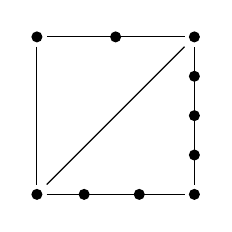
\begin{tikzpicture}
      \node (n1) at (0,0) {};
      \node (n2) at (2,0) {};
      \node (n3) at (2,2) {};
      \node (n4) at (0,2) {};
      \node (n5) at (0.6,0) {};
      \node (n6) at (1.3,0) {};
      \node (n7) at (2,.5) {};
      \node (n8) at (2,1.0) {};
      \node (n9) at (2,1.5) {};
      \node (n10) at (1,2) {};
      \foreach \i in {1,...,10} {
	\fill (n\i) circle(2pt);
      };
      \foreach \i/\j in {1/2, 2/3, 3/4, 4/1, 1/3} {
	\path (n\i) edge (n\j);
      };
    \end{tikzpicture}
  }
  \caption{Graph $G$ and one possible subdivision of $G$ named $H$}
\end{figure}




% Kuratovski's theorem?
\Theorem.
\[
    G\text{ planar} \iff \nexists\;\text{subgraph which is a subdivision of $K_5$ or of $K_{3,3}$.}
\]

\ProofBackward. Trivial if $K_5$ and $K_{3,3}$ non-planar.

\ProofForward. Too hard.

\textbf{Remark (Euler's polyhedron formula).}
\[
    G\text{ connected and planar} \implies
    \underbrace{\alpha_0 - \alpha_1 + \alpha_2}_
        {\text{Euler characteristic}}
    = 2.
\]

% figure of a polyhedron of a dice

\begin{figure}[htb] % polyhedron of a dice
  \centering
    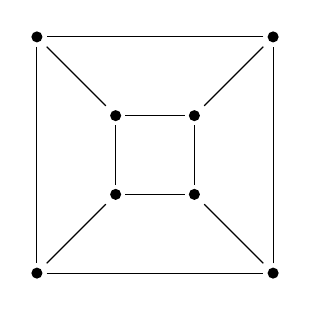
\begin{tikzpicture}
      \drawGraph{1/1, 2/1, 2/2, 1/2, %
                 0/0, 3/0, 3/3, 0/3}%
		{1/2, 2/3, 3/4, 4/1, %
                 5/6, 6/7, 7/8, 8/5, %
	         1/5, 2/6, 3/7, 4/8}
    \end{tikzpicture}
  \caption{Polyhedron of a dice}
\end{figure}





\Proof.
Induction on $\alpha_2$.

Start with $\alpha_2=1$: $G$ is a tree. Then
\[
    \alpha_0-\alpha_1+1 = \alpha_0 - (\alpha_0 + 1) + 1 = 2.
\]

$\alpha_2 = k : k\rightarrow k+1: $
\[
    \text{$G$ has at least $k+1 \geq 2$ faces} \implies
    \exists\;\text{edge separating two faces}
\]
If we remove this edge, we get $G'$.
\begin{align*}
    \alpha_2(G') = k
    \implies &\alpha_0(G') - \alpha_1(G') + \alpha_2(G') = 2
    \implies &\alpha_0(G) - \alpha_1(G) + \alpha_2(G) = 2
\end{align*}

\Lemma.
If $G$ is planar, simple, no cycles of length $3$ (together, this also means no cycles of length $≤ 3$), connected, then
\[
    \alpha_1(G) ≤ 2\alpha_0(G) - 4.
\]

\Proof. 
Let $f_j$ be the number of faces with a boundary of length $j$.
Then $f_3 = 0$.
\begin{align*}
\sum_{j≥4} f_j &= \alpha_2 \\
\sum_{j≥4} j f_j &≤ 2\alpha_1
    &&\text{ because each edge is counted at most twice.} \\
4 \sum_{j≥4} f_j ≤ 2\alpha_1
\end{align*}

%\TODO{figure 4 vertices, 3 faces}

\begin{align*}
    \alpha_0 - \alpha_1 + \alpha_2 &≥ 2 \\
    2\alpha_0 - 2\alpha_1 +
    \underbrace{2\alpha_2}_{≤ \alpha_1} &= 4 \\
    4 &≤ 2\alpha_0 - \alpha_1 \\
    \alpha_1 &≤ 2\alpha_0 - 4
\end{align*}

\Remark. In a graph with $k$ components, the Euler characteristic becomes
$\implies \alpha_0 - \alpha_1 + \alpha_2 = 1+k$

\textbf{Corollary.}
$K_{3,3}$ is not planar: Assume it is planar.
$\alpha_0 = 6, \alpha_1 = 9$. As a bipartite graph, it cannot have cycles of length 3: $f_3 = 0$. Therefore, we must have
\[
    \alpha_1 ≤ 2\alpha_0 - 4 \\
    9 ≤ 8
\]
Contradiction! Since $K_{3,3}$ satisfies all other requirements of the lemma, but the inequality does not hold, it cannot be planar.

\begin{definition}
Let $G=(V,E)$ be a planar graph and $F$ the set of faces.
Then $G^* = (V^*, E^*)$ is the \dt{dual} of $G$ with
\begin{align*}
&V^* = F. \\
&F_1F_2 \in E^* &&\text{if their boundaries have a common edge.}
\end{align*}
\end{definition}

% WRONG: \Remark. In general, $G^*$ is a multigraph.
\Remark. $G^*$ is not unique.
% WRONG: \Remark. $\forall v : d(v) ≠ 1 \implies |E| = |E^*|$


\subsection*{Bipartite Graphs and Matchings}

\begin{definition}
A simple, undirected graph $G=(V,E)$ is called \dt{bipartite}
iff
\begin{align*}
    V = V_1\cup V_2, V_1\cap V_2 = \varnothing \\
    vw\in E\implies v\in V_1, w\in V_2
\end{align*}
\end{definition}

$K_{n,m}$ is the complete bipartite graph.

\begin{definition}
$M\subseteq E$ is called a \dt{matching} if
\[
    \forall e,f\in M: e,f\text{ have no vertex in common.}
\]
\end{definition}
\begin{definition}
In a \dt{perfect matching},
\[
    \forall v\in V: v\text{ incident to some }e\in M.
\]
\end{definition}

\begin{figure}[htb] % perfect matching
  \centering
    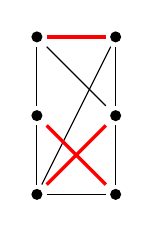
\begin{tikzpicture}
      \drawGraph{0/0, 0/1, 0/2, 1/0, 1/1, 1/2}%
                {1/2, 2/3, 1/6, 1/4, 3/5, 4/5, 5/6}
      \foreach \i/\j in {1/5, 2/4, 3/6} {
	\draw[red, very thick] (n\i) -- (n\j);
      };
    \end{tikzpicture}
  \caption{Graph with perfect matching in red}
\end{figure}




%%% EtherPad for Discrete Mathematics VO
%%% http://www.informatik-forum.at/showthread.php?104454-Notes-2013WS-VO_01
%%% Past pads:
%%%     * 2013-10-17: committed by patrikf
%%%     * 2013-10-18: committed by patrikf

% Discrete Mathematics Lecture Notes 2013-10-24

\def \GammaPlus {\Gamma^{+}}

\Remark.
\begin{compactenum}
  \item $|E| = |E^*|$
  \item In general $|G^*|$ is a multigraph
  \item $G_1, G_2$ are duals of $G \Rightarrow G_1 \cong G_2$
\end{compactenum}

$A \subseteq E$    
$A$ cycle in $G \iff A^*$ minimal cut

If G is not necessarily planar: define $G^*$ by (*).
This Graph is unique, if it exists.

\textbf{Theorem (Witness Theorem).} \\
If G is not necessarily planar: define $G^{**}$ by (*)
\begin{compactitem}
  \item $G$ planar $\Rightarrow G^{**} \cong G^*$
  \item $G$ non planar $\not\exists G^{**}$
\end{compactitem}
% end of last weeks-corrections


\subsection*{Matchings and Bipartite Graphs}

\strut\lecturedate{2013-10-24}
\textbf{Theorem (Hall's marriage theorem).}
$W, M$ (women, men) vertex set of a bipartite graph
($V=W\cup M$, $wm \in E \iff wFm$). $W,M$ finite, nonempty, $W\cap M=\varnothing$.

Friendship relation $F\subseteq W\times M$.

Feasible marriage: complete matching $F_1\subseteq F$, i.e.
\[ \forall x\in W: \exists! y\in M\text{ s.t. }x\operatorname{F} y \]

Theorem: There is a feasible marriage iff
\[
    \forall W_0\subseteq W:
        \underbrace{
            |\{y\in M\mid \exists x\in W_0: x\operatorname{F} y\}|
        }_{\Cup_{w\in W_0} \Gamma(w)}
        ≥ |W_0|
\]

if you have a feasable marriage, every woman gets a partner.
The Set of friends is at least this large

\textbf{Proof.}
Consider the network source $s$ $\rightarrow_{w=1}$ women $\rightarrow_{w=|W|+|M|+1}$ men $\rightarrow_{w=1}$ sink $t$.
Since all weights are integer, $\exists$ maximal flow with integer weight.

\begin{figure}[htb]
  \centering
  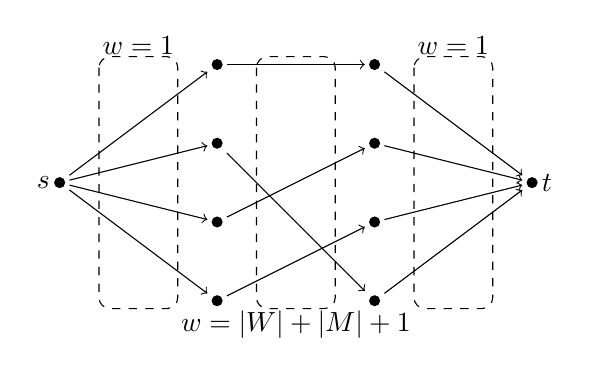
\begin{tikzpicture}
    \drawDirGraph{0/0, 2/1.5, 2/0.5, 2/-0.5, 2/-1.5, 4/1.5, 4/0.5, 4/-0.5, 4/-1.5, 6/0}%
      { 1/2, 1/3, 1/4, 1/5, %
        6/10, 7/10, 8/10, 9/10, %
        2/6, 3/9, 4/7, 5/8}
    \draw[rounded corners,dashed] (1-0.5, 1.6) rectangle (1+0.5, -1.6);
    \draw[rounded corners,dashed] (5-0.5, 1.6) rectangle (5+0.5, -1.6);
    \draw[rounded corners,dashed] (3-0.5, 1.6) rectangle (3+0.5, -1.6);
    \node at (n1)[left] {$s$};
    \node at (n10)[right] {$t$};
    \node at (1,1.5)[above] {$w=1$};
    \node at (5,1.5)[above] {$w=1$};
    \node at (3,-1.5)[below] {$w=|W| + |M| + 1$};
  \end{tikzpicture}
  \caption{feasable marriage, $\exists$ maximal flow with integer weights}
\end{figure}


We claim that $S=(\{s\}, V \setminus \{s\})$
is a minimal cut ($c(S) = |W|$).

Assume $\exists S': c(S') < c(s)$. Then $S'$ has no edge $wm$ with $w\in W, m\in M$.

\[
S' = (V_1,V_2) ^=
    \{sw\mid w \in \widetilde{W} \subseteq W \} \cup
    \{mt | m \in \widetilde{M} \subset M \}
\]

We claim that
\[
    w\in W\setminus\widetilde{W}, m\in\GammaPlus(w)
    \implies m\in\widetilde{M}.
\]
Assume this does not hold. Then
\path{s, w, m, t} does not contain an edge of $S'$ $\implies s, t\in V_1$. Contradiction!

This implies that
\[
    |\Cup_{w\in W\setminus\widetilde{W}} \GammaPlus(w)|
    ≤ |\widetilde{M}|.
\]
But
\[
    c(S') = |\widetilde{W}| + |\widetilde{M}| < c(S) = |W|.
\]
This implies that
\[
    |\widetilde{M}| < |W\setminus \widetilde{W}|.
\]
Contradiction! Therefore $S'$ can not be a minimal cut. $S$ is proven to be a minimal cut.

The theorem of Ford-Fulkerson says that with a minimal cut,
$\exists\;\text{flow }\phi: v(\phi) = c(S) = |W|$. This flow defines the feasible marriage relation.


\subsection*{Graph Colorings}

\begin{definition}
$G=(V,E)$ simple, undirected graph.
A \dt{vertex coloring} is a mapping
\[
    c : V\mapsto C, C=\{c_1,\ldots,c_r\}
\].
A coloring is \dt{feasible} if $vw\in E\implies c(v)≠c(w)$.
\end{definition}

\Remark. Edge coloring $\bar{c}: E\mapsto C$, feasible if edges with a common vertex have different colors.

\[
  \bar{G} = (\bar V, \bar E), \bar V = E
  e_1 e_2\in \bar E \iff e_1,e_2\text{ share common vertex}
\]

\Remark. Similarly, face colorings of a planar graph (think of a map of countries) can be 

\begin{definition}
$G=(V,E)$ graph. The \dt{chromatic number} $\chi(G)$ is the minimal number of colors so that there is a feasible coloring.
\end{definition}

Examples:
$\chi(K_n) = n$

$\chi(K_{n,m}) = 2$

$\chi(T) = 2$ if $T$ tree, $|V| ≥ 1$.

\Theorem.
\[
\begin{array}{r@{\quad}r@{ }l}
\text{1.} &
    \chi(G) = 1&\iff E(G) = \varnothing. \\
\text{2.} &
    \chi(G) = 2
        &\iff E(G) ≠ \varnothing, G\text{ bipartite} \\
        &&\iff E(G) ≠ \varnothing, \text{all cycles have even length}
\end{array}
\]

\Theorem.
$G$ planar $\implies \chi(G) \leq 4$. Proof is very hard!

\Theorem.
$\chi(G) ≤ 1 + \max{d(v)}.$

\Proof. By induction on $\alpha_0(G)$.

\Theorem. $G$ planar$\implies \chi(G) ≤ 5$.

\def\dmin{\ensuremath{d_{\text{min}}}}
\Proof.
Claim: In a planar graph, all vertices have at most five neighbors:
$\dmin ≤ 5$.

Assume $\dmin ≥ 6$.
Then
\[
  2\alpha_1 = \sum_{x\in V} d(x) ≥ 6\alpha_0
  \alpha_1 ≥ \alpha_0.
\]
\[
  2\alpha_1 ≥
  \sum_{\text{faces}} \text{number of boundary edges} ≥
  3\alpha_2 =
  3 (2 - \alpha_0 + \alpha_1)
\]
\[
  \alpha_1 ≤ 3\alpha_0 - 6
\]

But $\alpha_1 ≥ 3\alpha_0$! Contradiction.

Cases: \\
\begin{compactenum}
%Case 1:
  \item $\dmin \leq 4$. Pick $x_0$ so that $d(x_0) \leq 4$.
Take $G' = G \setminus \{x_0\}$. Assume $\chi(G')=5$. Then, since $x_0$ has at most $4$ neighbors, you can color $x_0$ with the remaining color. By induction, $\chi(G)=5$.

%Case 2:
  \item $d_{\text{min}}=5$.
We have a vertex $v$ with exactly 5 neighbours $\{a,b,c,d,e\}$.
$c(a) = 1, c(b) = 2,\ldots$.
\\
$G_a = \{x\in V\mid \exists 1--3--1--3--\ldots path a \leadsto x\}$.
Similar for $G_c$.
  \begin{compactenum}
%Case 2.1: 
    \item If $G_a\cap G_c =\varnothing$, we can recolor $G_a$ by switching colors 1 and 3. Then we can color $v$ with $c(v) = 1$.

%Case 2.2: 
    \item If $G_a\cap G_c ≠ \varnothing$, then $G_a = G_c$.
%Case 2.2.1:
    \begin{compactenum}
      \item If $G_b\cap G_d =\varnothing$, then recolor $G_b$ by switching 2 and 4, and $c(v) = 2$.
%Case 2.2.2: 
      \item If $G_b\cap G_d ≠\varnothing$, then $G_b = G_d$. Contradiction! (planar graph - the paths $G_a=G_c$ and $G_b=G_d$ cannot cross each other)
    \end{compactenum}
  \end{compactenum}
\end{compactenum}

\subsection*{Ramsey Theory}

\textbf{Example.} Every 2-edge coloring of $K_6$ has a monochromatic $K_3$.

\begin{figure}[htb]
  \centering
  \subfigure[$K_6$]{
    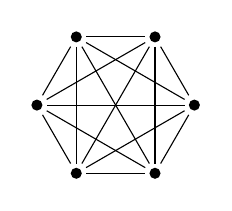
\begin{tikzpicture}
      \fullyConnectedGraph{90-30, 90+30, 0, 180, 270-30,270+30}{1cm}
    \end{tikzpicture}
  }
  \subfigure[$K_3$]{
    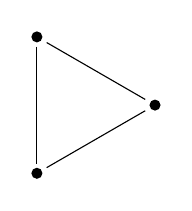
\begin{tikzpicture}
      \fullyConnectedGraph{90+30, 270-30,0}{1cm}
    \end{tikzpicture}
  }
  \caption{$K_6$ and one $K_3$}
\end{figure}

\TODO{Proof (graphical).}

\begin{definition}
The Ramsey number $R(r,s)$ is
\[
    R(r,s) =
        min \{n\mid \text{every red-blue coloring of $K_n$ contains a red $K_r$ or a blue $K_s$}\}.
\]
\end{definition}

By our example, $R(3,3) ≤ 6$. We can even show that $R(3,3) = 6$.

\TODO{figure out a good caption for Figure $K_5$}
\begin{figure}[htb]
  \centering
  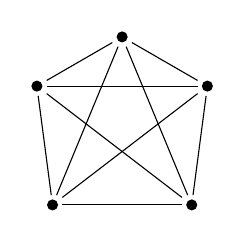
\begin{tikzpicture}
    \fullyConnectedGraph{90, 30, 180-30, -90-45, -90+45}{1.25cm}
  \end{tikzpicture}
  \caption{$K_5$}
\end{figure}

Lemma. $R(r,s) ≤ R(r-1, s) + R(r, s-1)$

Proof. $n = R(r-1, s) + R(r, s-1)$
Partition $K_n$. Take a vertex $v$. All neighbours connected by a red edge are in $M$; all neighbours connected by a red edge are in $N$.
n = |M|+|N|+1. Thus
|M| ≥ R(r-1, s) or |N| ≥ R(R, s-1).

\begin{tabular}{ll}
  Case 1: & $\exists$ blue $K_s$ in $M$ or $\exists$ red $K_{r-1}$ in $M$. \\
  Case 2: & $\exists$ blue $K_{s-1}$ or red $K_r$ in $N$.
\end{tabular}

We wanted to show that $\exists$ blue $K_s$ or $\exists$ red $K_r$.
In both cases, \emph{together with $v$}, we can always find a blue $K_s$ or a red $K_r$.

\textbf{Corollary.} $R(r,s) ≤ \choose{r+s-2}{r-1} ≤ 2^{r+s-2}$

\Proof. $R(2,n) = R(n,2) = n ≤ \choose{n}{1}$. From there, apply induction, Pascal's triangle, and the above lemma.

\begin{definition}
\[
    R(n_1,n_2,\ldots,n_r) =
    \min \{ n \mid
        \text{all r-edge colorings of $K_n$
        (colors $c_1,\ldots,c_r$) have a
        $c_j$-colored $K_j$ for some j}
\]
\end{definition}












%%% EtherPad for Discrete Mathematics VO
%%% http://www.informatik-forum.at/showthread.php?104454-Notes-2013WS-VO_01
%%% Past pads:
%%%     * 2013-10-17: committed by patrikf
%%%     * 2013-10-18: committed by patrikf
%%%     * 2013-10-24: committed by patrikf

% Discrete Mathematics Lecture Notes 2013-10-25

\chapter{Higher Combinatorics}

\section{Enumerative Combinatorics}

$A$ finite set, $|A|$ = ?

$(A_n)_{n ≥ 0}$ system of finite sets, $a_n = |A_n|$, what is the \dt{counting sequence} $(a_n)_{n ≥ 0}$

The goal might be to find
\begin{compactitem}
\item a closed formula (often impossible),
\item a recursion,
\item a generating function (e.g. $\sum_{n >= 0}[a_n z^n]$),
\item asymptotic estimates, $a_n$ symptotically similar to $b_n$:
    $a_n \sim b_n \iff \lim_{n \to \inf} \frac{a_n}{b_n} = 1$
\end{compactitem}


\textbf{example}
\begin{align*}
A_n &= \{permutations of 1,2, \ldots, n\}, |A_n| = n! \\
a_1 &= 1, a_n = n a_{n-1} \\
a_n \sim (\frac{n}{e})^n \sqrt{2\pi n}
\end{align*}


\subsection{Counting principles}

Elementary counting principles:
% TODO make subsubsections out of this
\begin{compactenum}
\item Sum principle:
    $A\cap B = \varnothing \implies |A\cup B| = |A| + |B|$
\item Product principle:
    $|A\times B| = |A| * |B|$
\item Bijection principle:
    $f: A\mapsto B, \text{bijective}\implies |A| = |B|$
\end{compactenum}

\textbf{Example.}
What is the number of two-digit positive integers?
$|\{10,\ldots,99\}| = 90$

\begin{gather*}
xy\quad x\in X=\{1,2,\ldots ,9\}, y\in Y = \{0,1,\ldots ,9\} \\
|X\times Y| = |X| \cdot |Y| = 9\cdot 10 = 90
    \qquad\text{(product principle)}
\end{gather*}

\textbf{Example.}
We choose a password with 4 to 10 digits. How many passwors are possible?

\begin{align*}
    A_i &&& \text{set of passwords with $i$ digits} \\
    Y &= \{0,1,\ldots ,9\} \\
    A_i &= Y^i, |Y| = 10, |A_i| \\
    &= {10}^i  && \text{(product principle)} \\
    \text{total number} &= 10^4 + 10^5 + \ldots + 10^10 && \text{(sum principle)}
\end{align*}

\textbf{Example.}
There is a Thief, which saw me using a bank-card, and afterwards stole this card. He saw the code starts with $0$ and contains an $8$. How many possibilities for the password?

4 Digits ($0 \ldots$), with the product principle we get $10^3$ options. 

Using the sum principle we can subtract codes the containing $8$.

\begin{align*}
|A| &= \text{\# possibilities} \\
	&= \underbrace{|A\cup B| - |B|}_{\text{(sum principle, reversed)}} \\
    &= {10}^3 - \text{\# codes not containing 8} \\
    &= {10}^3 - 9^3 = 271.
\end{align*}

\textbf{Example.}
Take a set $A = \{a_1, a_2, \ldots , a_n\}$ and its power set $2^A = \{X \mid X
\subseteq A\}$. $|2^A| = ?$

\begin{align*}
    B &\subseteq A \\
    i_k &\quad\text{indices chosen from A} \\
    B &=\{a_{i_1}, a_{i_2},\ldots, a_{i_k}\} \\
    k &\leq n, 1 \leq i_1 < i_2 < \ldots i_k \leq n
        B &\mapsto
        (b_1, b_2 \ldots  b_n) \in \{0,1\}^n \\
    b_i &=
    \begin{cases}
        1 & a_i\in B \\
        0 & a_i\not\in B
    \end{cases} \\
    f: 2^A &\mapsto \{0,1\}^n &&\text{bijective mapping} \\
    |2^A| &= |\{0, 1\}^n| = 2^n
        &&\text{(bijection principle)} \\
\end{align*}

\subsubsection{Double counting}
If:
\begin{align*}
	A &= \{a_1,a_2,\ldots,a_m\} \\
	B &= \{b_1,b_2,\ldots,b_n\} \\
	R & \subseteq A \times B \\
	\text{Set } R_{i,0} &= \{b \in B \mid a_i\operatorname{R} b\}  && \text{(subscript 0 just means}\\
	\text{Set } R_{0,i} &= \{ a \in A \mid a\operatorname{R} b_i \}  && \text{that this part is fixed)}
\end{align*}
	

%Set R_{i,0} = \{b \in B \mid (a_i,b) \in R\}
Then:
\begin{align*}
	|R| &= \sum_{i=1}^m |R_{i,0}|\\
     &= \sum_{j=1}^n |R_{0,j}|
\end{align*}

\textbf{Proof.}
Define matrix $(x_{ij})_{i = 1,\ldots,m; j = 1,\ldots ,n}$ with

\[x_{ij} = \begin{cases}
        1 & a_i\operatorname{R} b_j \\
        0 &\text{otherwise}
    \end{cases}\]

The first sum is the row-wise sum, the second sum column-wise. Of course, summing up all the elements of the matrix, you get the same result. In some problems, this equivalence may be helpful, because one of the sums is easier to compute than the other.


\textbf{Example.}
\begin{align*}
    \tau(n) &= \text{average number of divisors of an integer k}, 1 ≤ k ≤ n \\
    d(n) &= \text{ number of divisors of n} \\
    \tau(n) &= \frac{d(1)+\ldots+d(n)}{n} \\
        &= \frac1n\sum_{i=1}^n d(i)
\end{align*}

\bigskip
\begin{table}[H]
\begin{center}
\begin{tabular}{r|ccccccccc}
\toprule
$n$    &1&2&3&4&5&6&7&8&9 \\
$d(n)$ &1&2&2&3&2&4&2&4&3 \\
\bottomrule
\end{tabular}
\caption{The number of divisors for every number from $1$ to $9$. $\text{E.g.: } n = 6, \tau(6) = \frac{7}{3}$}
\end{center}
\end{table}

\begin{align*}
A &= B = \{1,\ldots,n\} \\
R & \subseteq A\times B :\ a\operatorname{R} b\iff a|b && \text{ ($a$ divides $b$)}
\end{align*}
\bigskip

One may write down $\operatorname{R}$ as a matrix:

\begin{table}[H]
	\begin{center}
		\begin{tabular}{l|cccccc}
			\textbf{1} & \textbf{2} & \textbf{2} & \textbf{3} & \textbf{4} & \textbf{5} & \textbf{6} \\
			\hline \textbf{1} & 1 & 1 & 1 & 1 &  1 & 1 \\
			\textbf{2} & 0 & 1 & 0 & 1 &  0 & 1 \\
			\textbf{3} & 0 & 0 & 1 & 0 &  0 & 1 \\
			\textbf{4} & 0 & 0 & 0 & 1 &  0 & 0 \\
			\textbf{5} & 0 & 0 & 0 & 0 &  1 & 0 \\
			\textbf{5} & 0 & 0 & 0 & 0 &  0 & 1
		\end{tabular}
		\caption{Table of relations ``a divides b'' for the numbers 1 to 6.}
	\end{center}
\end{table}

\begin{align*}
\text{$n$ prime}
    &\implies d(n) = 2 \\
n = p^e, p\in \mathbb{P}, e\in \mathbb{N}^{+}
    &\implies d(n) = e+1 \\
n = \prod_{i=1}^k p_i^{e_i}
    &\implies d(n) = \prod_{i=1}^k (e_i+1)
\end{align*}

(Because of $l | n \iff l = \prod_{i=1}^k p_i^{f_i},
f_i ≤ e_i$, l is defined by $(f_1,\ldots,f_k)$.)

\begin{align*}
\tau(n) &= \frac{1}{n}\sum_{i=1}^n d(i)\\
    &= \frac{1}{n}\sum_{j=1}^n |R_{0,j}| && \text{(sum of columns)} \\
    &= \frac{1}{n}\sum_{i=1}^n |R_{i,0} && \text{(sum of rows)}
\end{align*}

\begin{align*}
R_{0,j} &= \{a \mid a \operatorname{R} j\} = d(j) \\
R_{i,0} &= \{b \mid i\operatorname{R} b\}
    = \text{sum of the number of multiples of $i$ in $b$}
\end{align*}

\begin{align*}
\tau(n) = ... &=
    \frac{1}{n} \sum_{i=1}^n \lfloor\frac{n}{i}\rfloor \\
    &= \frac{1}{n} \sum_{i=1}^n (\frac{n}{i} -
        \underbrace{\{\frac ni\}}_{\text{fractional part}} \\
    &= \sum_{i=1}^n \frac1i -
        \frac1n\sum_{i=1}^n
            \underbrace{\{\frac ni\}}_{≤ 1} \\
    &=  \underbrace{H_n}_{\begin{matrix}harmonic \\ numbers\end{matrix}} + O(1) =
        \log n + e_n (e ... error), -1 < e_n < 1 && H_n\sim \log n
\end{align*}


\subsubsection{Pigeon hole principle}

$A_1, \ldots , A_k$ finite pairwise disjoint set,
$|A_1 \cup \ldots \cup A_k| > k\cdot r$
$\implies \exists i : |A_i| > r$

If $r=1$, you can also say that
\[
    f: A\mapsto B, |A| > |B| \implies \exists b \in B :
    |\underbrace{f^{-1}(b)}_{\text{set of preimages of b}}|
        ≥ 2 ,
        \text{i.e. f is not injective}
\]


\textbf{Example.}
Claim: There are 2 people living in Austria who are born in the same hour of the same day in the same year.

\textbf{Proof.}
Possible hours: $365\cdot 24\cdot 200 < 2\cdot 10^6$;
the population is bigger than that.


\textbf{Example.}
Claim: $\forall q\text{ odd} \exists i: q | 2^i-1 =: a_i$.

\textbf{Proof.}
If $\exists i: a_i \cong 0 \mod q$, we are done.

Consider $a_1, a_2,\ldots, a_q \mod q$.
Either $\exists i: a_i \cong 0 \mod q$,
or $\exists i,j: i < j, a_i \cong a_j \mod q$
by the pigeon hole principle (without 0, only $q-1$ residue classes left)

Let's assume $i < j$, than:

\begin{align*}
a_i - a_j &= q\cdot a, a\in\mathbb{Z} \\
2^i(1 - 2^{j-1}) &= q\cdot a
\end{align*}

Since q is odd, $gcd(2^i, q)=1$. Therefore $q | 2^{j-1} - 1$. But in this case, $a_{j-i}\cong 0$!


\textbf{Example (Interpreting the pigeon hole principle as a colouring).}
$A$ set, $|A| = n$,
$l_1, l_2, \ldots, l_k ≥ 1 and n > l_1 + l_2 + \ldots + l_k - k$

By the pigeon hole principle, for each coloring of the elements of $A$ with colours 1 to $k$, there is an $i$ such that $l_i$ elements have the colour $i$.

\textbf{Proof.}
\[
    f: A\mapsto \{1,2,\ldots,k\}
\]
Assume
    $|f^{-1}(i)| = \text{\#elements having colour $i$} < l_i
    \quad\forall i$.
\[
	n = |A| = \sum_{i=1}^k |f^{-1}(i)| ≤ l_1 +\ldots + l_k - k
\]
Contradiction!


\subsubsection{Principle of Inclusion and Exclusion}

Given two non-disjoint sets $A$ and $B$  we may want to know the cardinality $|A \cup B|$.
The first idea which may come to one's mind could be to simply add up the cardinalities of $A$ and $B$:
$|A \cup B| = |A| + |B|$. However, this
is only true for disjoint sets. Given two overlapping sets, one will count the elements from
$A \cap B$ twice:

\begin{figure}[htb]
	\centering
	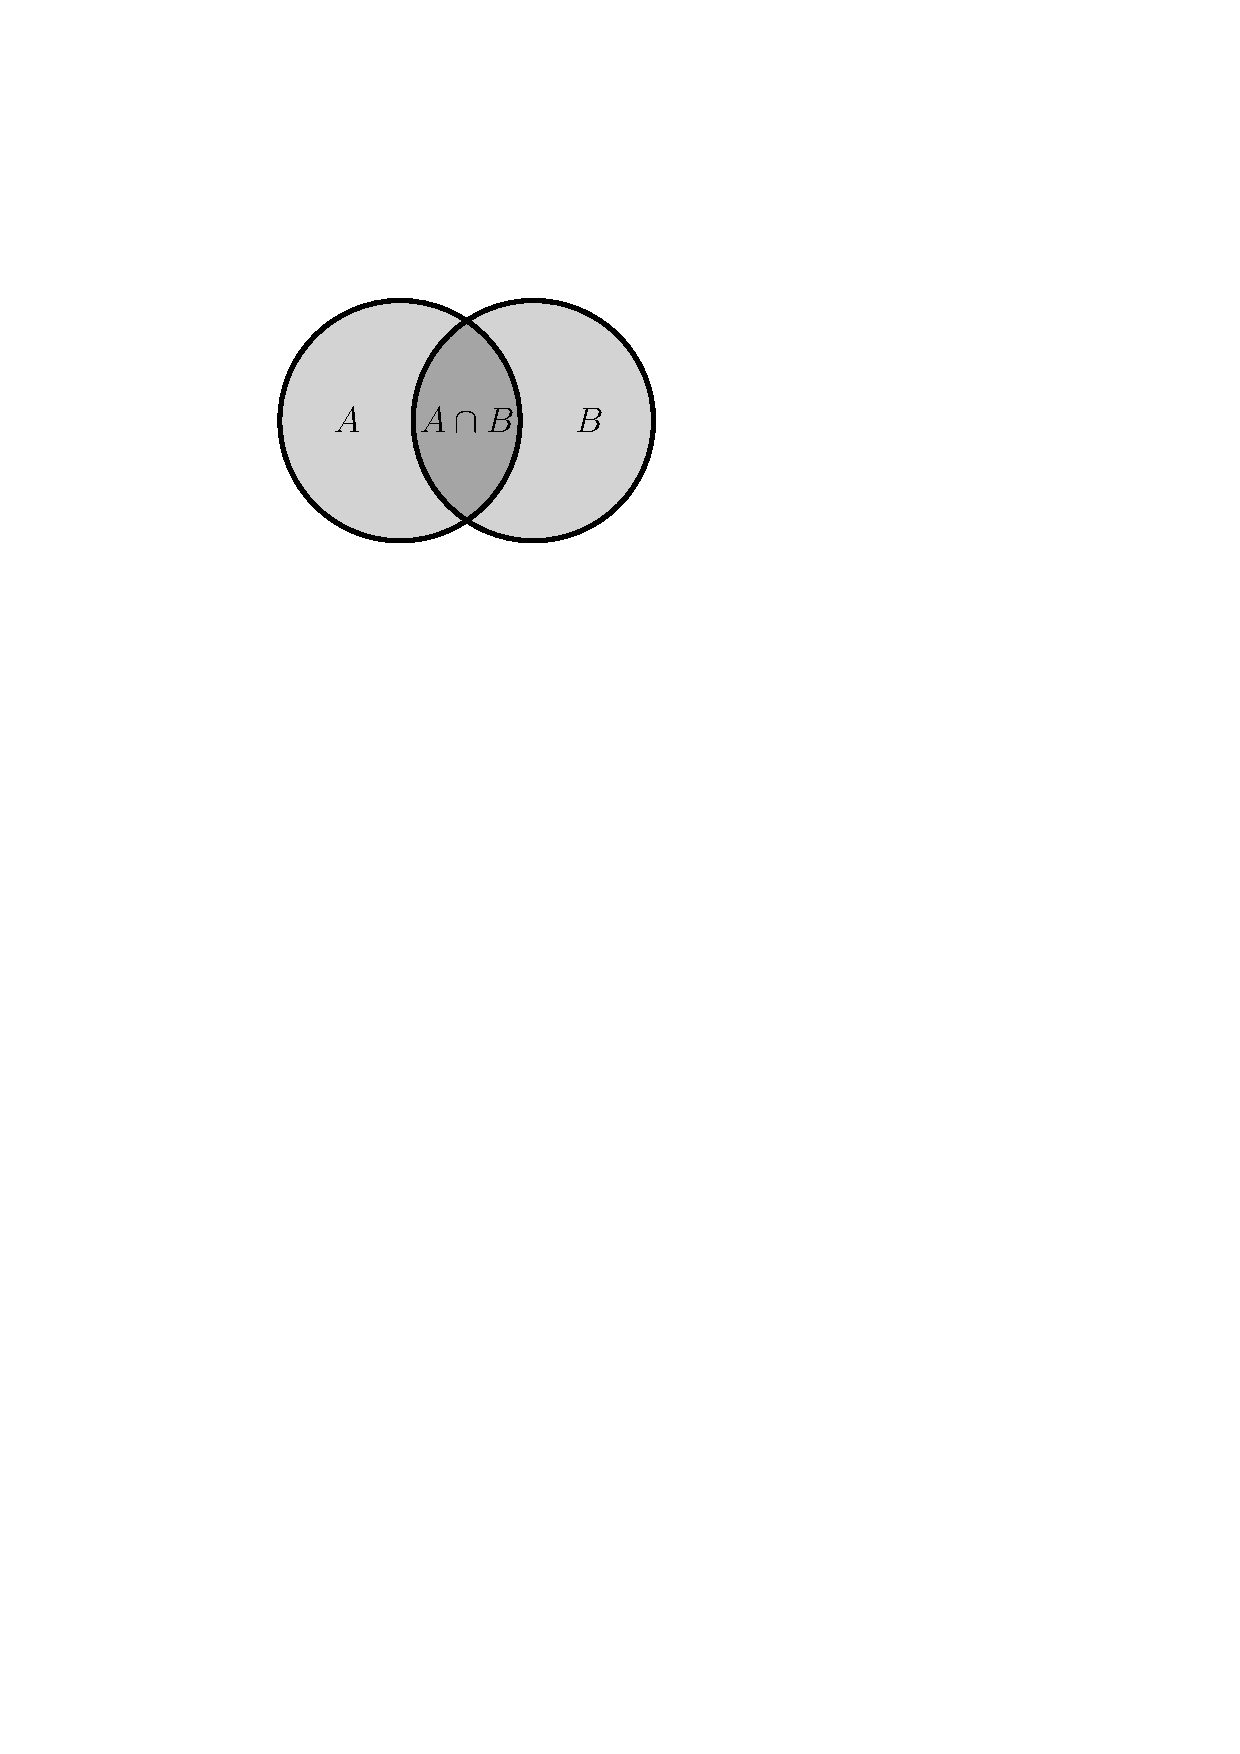
\includegraphics[scale=.5]{02_higher_combinatorics/pics/a_cut_b.pdf}
	\caption{When adding $|A|$ and $|B|$, the elements of $A \cap B$ will be counted twice.}
\end{figure}                                                                                                                                                                                                                                                        

In order to calcucate the cardinality of $|A \cup B|$ correctly we have to substract
$|A \cap B|$ from $|A| + |B|$:
\[
	|A \cup B| = |A| + |B| - |A \cap B|
\]

Now let's consider 3 overlapping sets $A$, $B$ and $C$. By simply adding up the cardinalities
$|A \cup B \cup C| = |A| + |B| + |C|$ once again many elements are double- or triple-counted:

\begin{figure}[htb]
	\centering
	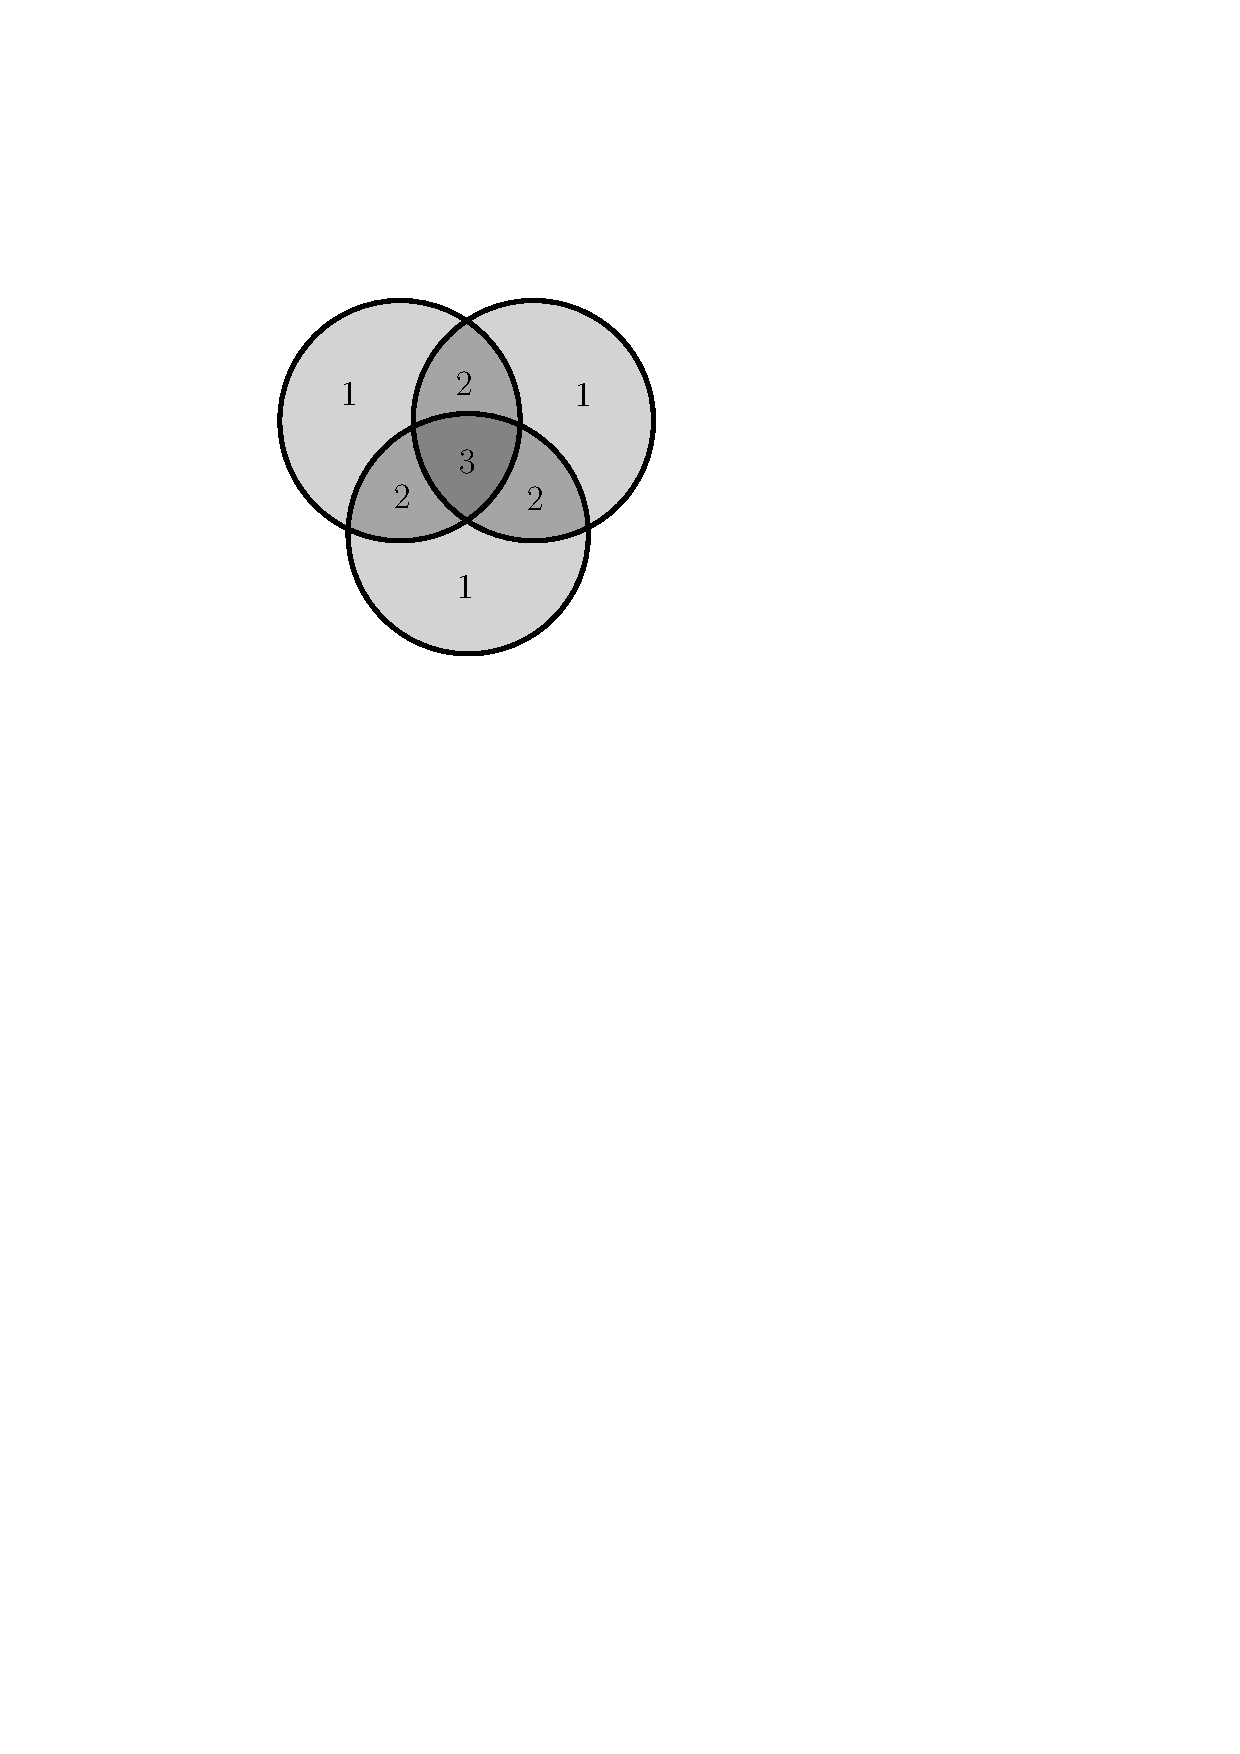
\includegraphics[scale=.5]{02_higher_combinatorics/pics/a_cut_b_cut_c.pdf}
	\caption{The numbers state, how often a certain area of $A \cup B \cup C$ has been counted by simply adding up $|A| + |B| + |C|$.}
\end{figure}

By substracting the number of elements of the cuts that were counted twice (namly $A \cap B$, $B \cap C$ and $C \cap A$) from $|A| + |B| + |C|$
we observe, that we now neglect the cut $A \cap B \cap C$ (because it had been counted 3 times before and we substract it's elements three times):

\begin{figure}[htb]
	\centering
	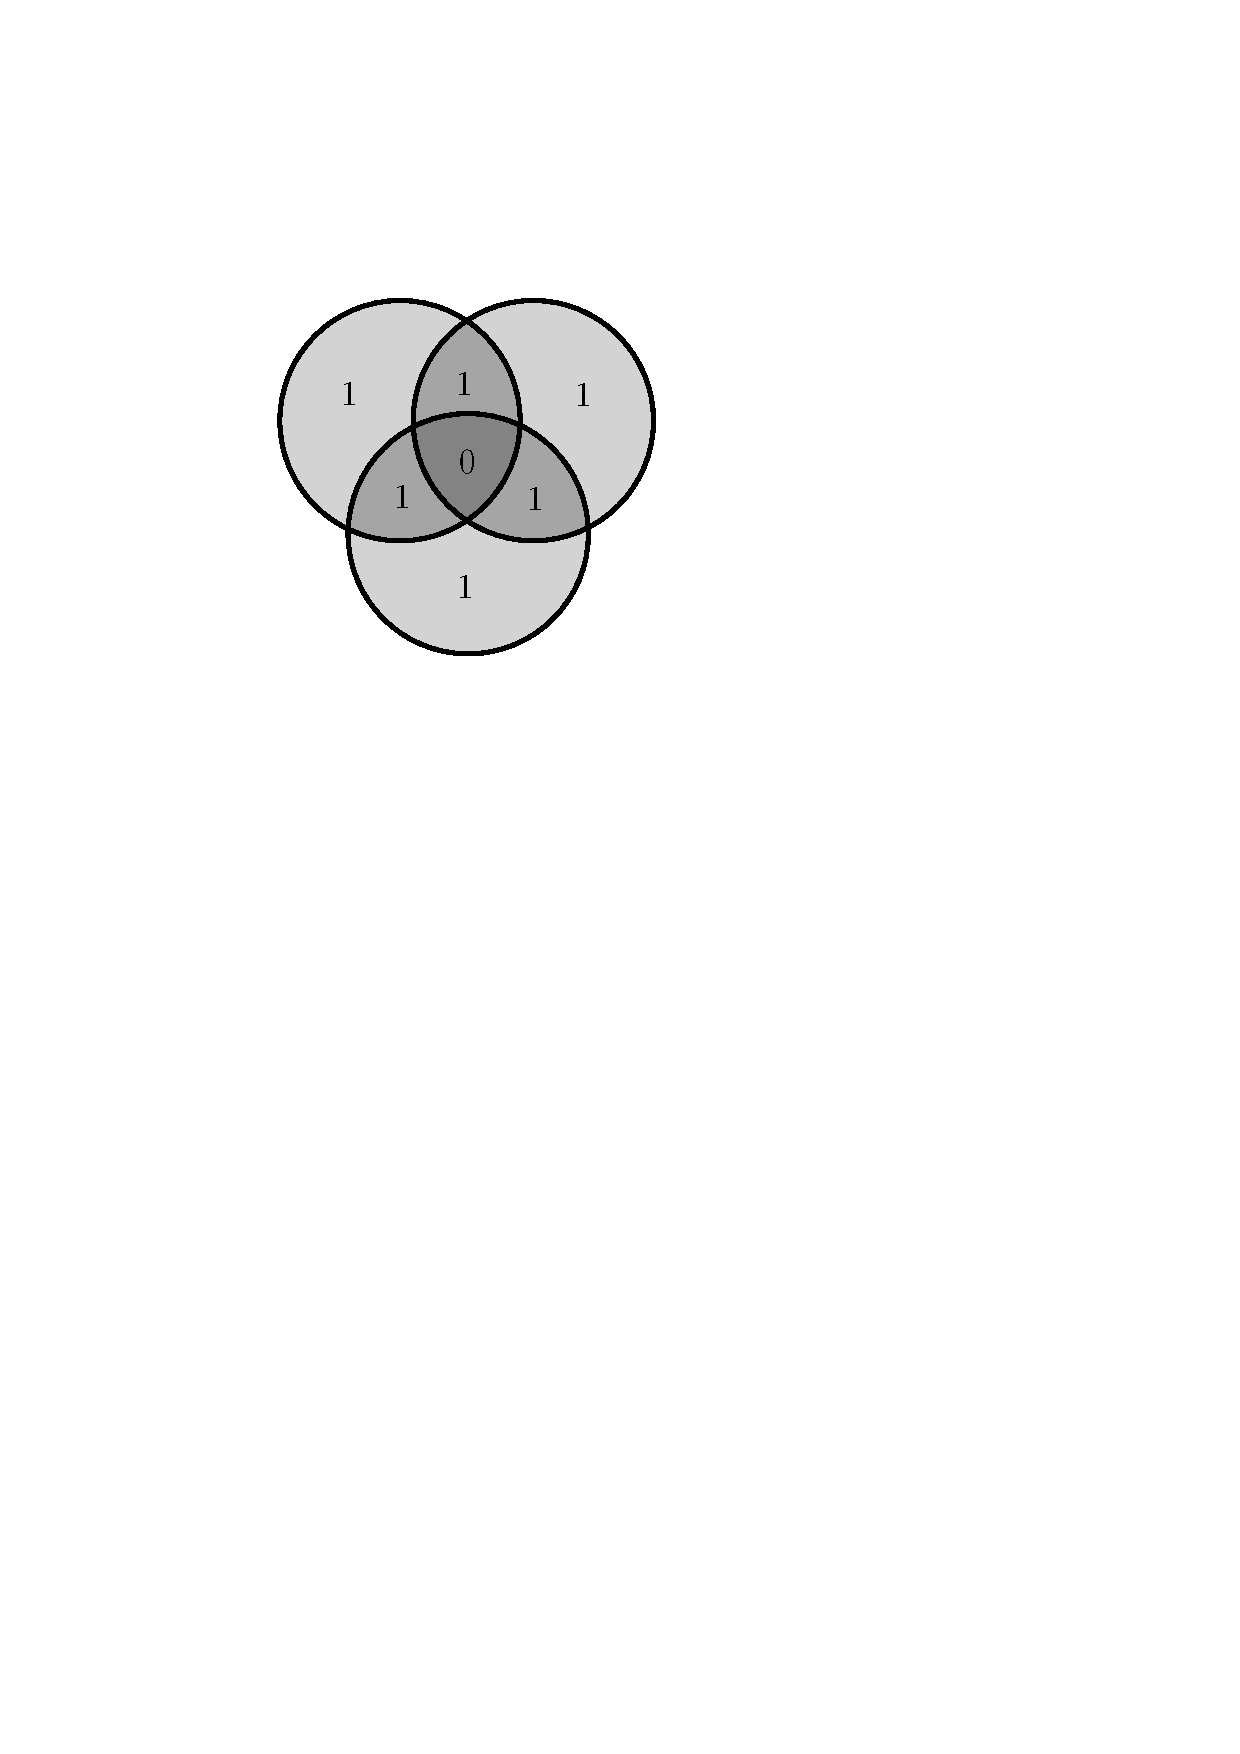
\includegraphics[scale=.5]{02_higher_combinatorics/pics/a_cut_b_cut_c_2.pdf}
	\caption{The numbers state, how often a certain area of $A \cup B \cup C$ has been counted by using the equation $|A| + |B| + |C| - |A \cap B| - |B \cap C| - |C \cap A|.$}
\end{figure}

So we have to add the number of elements of this cut again to get the correct number of elements in $A \cup B \cup C$.
All in all we get:

\[
	|A \cup B \cup C| = |A| + |B| + |C| - |A \cap B| - |B \cap C| - |C \cap A| + |A \cap B \cap C|
\]


With pairwise disjoint sets, we know that

\begin{align*}
|A_1\cup \cdots\cup A_n| &= |A_1| + \ldots + |A_n|.\\
|A_1\cup \cdots\cup A_n| &=
    \sum_{\varnothing\neq I\subseteq\{1,\ldots,n\}}
            (-1)^{|I|+1}
            \left|
            \bigcap_{i\in I} A_i
        \right|
\end{align*}

If we have a universe $A$ such that
\[
    A_1,\ldots,A_n \subseteq A
\]then

\begin{align*}
|A\setminus \Cup_{i=1}^m A_i| &=
|A| +
    \sum_{\varnothing\neq I\subseteq\{1,\ldots,n\}}
        (-1)^{|I|}
        \left| \bigcap_{i\in I} A_i \right| \\
&=
\sum_{I\subseteq\{1,\ldots,n\}}
    (-1)^{|I|}
    \left| \bigcap_{i\in I} A_i \right| \\
\end{align*}
... if you presume that "the intersection of nothing" is "everything" (A)































%%% EtherPad for Discrete Mathematics VO
%%% http://www.informatik-forum.at/showthread.php?104454-Notes-2013WS-VO_01
%%% Past pads:
%%%     * 2013-10-17: committed by patrikf
%%%     * 2013-10-18: committed by patrikf
%%%     * 2013-10-24: committed by patrikf
%%%     * 2013-10-25: committed by patrikf

% Discrete Mathematics Lecture Notes 2013-11-08

\subsection{Counting sets}
\lecturedate{2013-11-08}
Finite Set $A = \{a_1, \ldots, a_n\}$, $n$-element-set or $n$-set

A \dt{counting set} is a set $A = \{1, 2, \ldots, n\}$

\begin{enumerate}
  \item number of permutations: $n!$
  \item number of $k$-subsets: ${n\choose k}$
  \item number of ordered $k$-subsets: $k! {n\choose k}$
  \item number of $k$-multisets: $b_1, \ldots, b_k \in A$, the order doesn't matter, but we are allowed to choose a element several times $\implies$ ${n +k-1 \choose k}$
\end{enumerate}

There is a mapping $f$ that maps the
\[
  \text{$k$-multiset}
  \subseteq A:
  b_1 ≤ \ldots ≤ b_k
\]
to the
\[
  \text{$k$-subset}
  \subseteq \{1,2,\ldots,n+k-1\}:
  b_1 < b_2+1 < \ldots < b_k+k-1.
\]

\begin{enumerate} 
  \setcounter{enumi}{4}
  \item number of arrangements of a multiset: $\{b_1, b_1, \ldots , b_2, b_2,\ldots, b_2, \ldots, b_m, b_m, \ldots b_m\}$ 
\end{enumerate}

$b_1$ appears $k_1$ times, ...; $n$ in total

Permutations of this multiset:
$\frac{n!}{k_1! k_2! \ldots k_m!}$

\begin{enumerate}
  \setcounter{enumi}{5}
  \item number of ordered $k$-multisets over $A$: $n^k$ \\
  (we take a fixed number of positions $k$ and for each position choose any element from $A$)
\end{enumerate}

Remember:
\begin{compactitem}
  \item $\sum_{k=0}^n {n\choose k} = 2^n$
  \item Pascal's triangle
  \item ${n\choose k} + {n\choose k+1} = {n+1 \choose k+1}$
  \item $\sum_{m=0}^n {m\choose k} = {n+1 \choose k+1}$
  \item $\sum_{k=0}^n {m+k \choose k} = {m+n+1 \choose n}$
\end{compactitem}

\[
  \forall x,y\in \mathbb{C}
  \forall n\in \mathbb{N}
  (x+y)^n = \sum_{k=0}^n {n\choose k} x^k y^{n-k}
\]

$b_1, \ldots, b_k$ \; ${n \choose k} = \frac{n(n-1) \ldots (n-k+1)}{k!}$

\textbf{Definition (Extension to complex numbers).}
Let $x\in \mathbb{C}, k\in\mathbb{N}$. Then we can define
\[
  {x\choose k} = \frac{
    x (x-1) \ldots (x-k+1)
  }{
    k!
  }
\]

\Lemma.
\[
  \forall k \in \mathbb{Z}, \forall x\in \mathbb{C}:
  {x\choose k} = {x-1 \choose k-1} + {x-1 \choose k}
\]
(with ${x \choose k} = 0$ for $k < 0$).

\Theorem. (Vandermonde's theorem).
\[
  {x+y \choose n} = \sum_{k=0}^{n} {x\choose k} {y\choose n-k},
  \forall n \in \mathbb{N}, \forall x,y \in \mathbb{C}
\]

\Proof.
Assume $x,y\in \mathbb{N}$. $X,Y$ sets: $X\cap Y=\varnothing, |X|=x, |Y|=y$.

Then the left-hand side
${x+y \choose n}$
is the number of $n$-subsets of $X\cup Y$.

Choose any $n$-subset $A\subseteq X\cup Y$.
Then $A$ can be decomposed like this:
\begin{gather*}
  A = (A\cap X)\cup (A\cap Y) \\
  |A\cap X| = k, |A\cap Y| = n-k
\end{gather*}

number of unions of shape right hand side of (*) $\left(={x+y \choose n} \right)$

\[
  \sum_{k=0}^n {x\choose k} {y\choose n-k}
\]

left hand side: 
\[
  \sum_{i\in I} p_i (x) y^i
  = \sum \widetilde p_i (x) y^i
\]

lets assume $x\in \mathbb{N}$ and is fixed, then
\[
  Q_1(y) = Q_2(y) \; forall y \in \mathbb{N} 
  \implies \forall y\in \mathbb{C}
  p_i(x) = \widetilde p_i(x) \; \forall x \in \mathbb{N}
\]

\subsection{Stirling numbers}
Assume we have a set $A = \{1,2,3, \ldots ,n\}$
, permutation $\pi\in S_n$.
$S_n$ is the symmetric group; $|S_n| = n!$

We can represent $\pi$ as follows:
\[
  \begin{pmatrix}
    1&2&3&\cdots&n \\
    \pi(1)&\pi(2)&\pi(3)&\cdots&\pi(n) \\
  \end{pmatrix}
\]

2-line representation:
\[
  \begin{pmatrix}
    1&2&3&4&5&6&7 \\
    4&6&3&1&7&5&2 \\
  \end{pmatrix}
\]
The second line is also called the word representation.

Cycle representation:
$(1 4) (2 6 5 7) (3)$
Fixpoints can be omitted, so this is the same as $(14)(2657)$.

We can do calculations with permutations.

$(12)\in S_7 \implies (12)(3)(4)(5)(6)(7)$

A transposition is a permutation of just 2 elements.

Take $(12),(13)\in S_7$. Then $(12)\circ (13) = (132)$.

Every $\pi\in S_n$ can be written as a product of cycles, even as a product of transpositions (but not unique).

e.g. $(14)(2657) = (14)(27)(25)(26)$.

Of course, the order within a cycles does not matter:
$(2652)=(5726)$.

Canonical representation: generated from 2-line representation, smallest element comes first.
If additionally you start with the cycle with the largest last element first, you could even omit parentheses.

\begin{definition}
Let
\[
  s_{n,k} = \text{number of permutations of an $n$-set $A$ which have $k$ cycles}
\]
Then $s_{n,k}$ are the \dt{Stirling numbers of the first kind}.
(Fixpoints count as a cycle as well.)
\end{definition}

\Remark.
\begin{gather*}
  s_{n,1} = (n-1)! \\
  s_{n,n-1} = {n\choose 2} \\
  s_{n,n} = 1 \\
  s_{n,0} = s_{k,0} = 0 \quad n,k ≥ 1 \\
  s_{0,0} := 1 \\
  \sum_{k=0}^{n} s_{n,k} = n! 
\end{gather*}

It doesn't matter where we start the cycle, just the order of the cycle needs to stay. $(3 2 6 5 7 1 4) = (6 5 7 1 4 3 2)$

\Theorem.
\[
  \forall n,k > 0:\;
  s_{n,k} = s_{n-1,k-1} + (n-1)s_{n-1,k}
\]

\Proof.
Take a permutation 
$\pi = (1 \ldots )(\ldots) \ldots (\ldots) \in S_n \text{, with $k$ cycles}$.

How many such permutations are there?

\begin{compactitem}
  \item If $1$ is a fixed point: $s_{n-1, k-1}$.

  \item If $1$ is not a fixed point, start with a permutation of $n-1$ elements and add the element $1$ to one of the cycles. We can insert it before any of the $n-1$ elements, thus we get
$(n-1) s_{n-1,k}$ possibilities.
\end{compactitem}

\Remark.
Signed Stirling numbers of the first kind:
\[
  c_{n,k} = (-1)^{n+k} s_{n,k}
\]

\begin{definition}
Set partitions: 
Take a set $A=\{1,2, \ldots, n\}$
and decompose it such that
\[
  A = A_1 \cup A_2 \cup \cdots\cup A_k
  \quad
  \forall i\neq j: A_i \cap A_j = \varnothing
\]
Then
\[
  S_{n,k} = \text{number of set partitions of $A$ with $k$ blocks}
\]
are the \dt{Stirling numbers of the second kind}.
\end{definition}

\textbf{Example.}
Set $A = \{1,2,3,4\}$
\begin{align*}
  \text{number of 1-partitions }= 1 &= S_{4,1}\\
  \text{number of 2-partitions }= 7 &= S_{4,2}\\
  \text{number of 3-partitions }= 6 &= S_{4,3}\\
  \text{number of 4-partitions }= 1 &= S_{4,4}
\end{align*}

\Remark.
\begin{align*}
  S_{n,1} &= S_{n,n} = 1 \\
  S_{n,2} &= 2^{n-1}-1 \\
  S_{n,n-1} &= {n\choose 2} \\
  S_{0,0} &:= 1 \\
  S_{n,0} &= S_{0,k} = 0
    \quad\forall n,k ≥ 1
\end{align*}

\Theorem.
\[
  S_{n,k} = S_{n-1,k-1} + k S_{n-1,k}
\]

\Proof.
If $\{1\}$ is a block:
\[
  S_{n-1,k-1}
\]
If $\{1\}$ is not a block, it has to be element of one of the $k$ blocks:
\[
  k S_{n-1,k}
\]

\Theorem.
$\forall x\in \mathbb{C} \forall n ≥ 0:$
\begin{gather*}
  (x)_n
    := x(x-1)(x-2) \ldots(x-n+1)
    = \sum_{k=0}^{n} (-1)^{n+k} s_{n,k} x^k \quad ((x)_0:=1)
    \\
  x^n = \sum_{k=0}^{n} S_{n,k} (x)_k
\end{gather*}

\Remark.
$V_n = \{a_0 + a_1 x + \ldots + a_n x^n \mid a_i \in \mathbb{C} \}$ \\
$\{1,x,x^2, \ldots , x^n\}, \{1,(x)_1, (x)_2, \ldots ,(x)_n\}$ are bases of $V_n$ \\
$(V_n, +, \mathbb{C})$ vector space dim $V_n = n+1$

basis change: 
\[
  (S_{m,k})_{m,k= 0, \ldots,n} 
    ((-1)^{m+k} s_{m,k})_{m,k= 0, \ldots,n}
\]

\Proof.
\begin{align*}
  (x)_n
  &= (x)_{n-1} (x-n+1) \\
  &= (x-n+1) \sum_{k=0}^{n-1} (-1)^{n-1+k} s_{n-1,k} x^k \\
  &= \sum_{k=0}^{n-1} (-1)^{n-1+k} s_{n-1,k} x^{k+1} 
    + (n-1)\sum_{k=0}^{n-1} (-1)^{n+k} s_{n-1,k} x^k \\
  &= \sum_{k=1}^n (-1)^{n+k} s_{n-1,k-1} x^k
    \quad + (n-1)\sum_{k=0}^{n-1} (-1)^{n+k} s_{n-1,k} x^k \\
  &= \sum_{k=0}^n (-1)^{n+k}
    (s_{n-1,k-1} + (n-1)s_{n-1,k}) x^k \\
  &= \sum_{k=0}^n (-1)^{n+k} s_{n,k} x^k \\
\end{align*}


%%% EtherPad for Discrete Mathematics VO
%%% http://www.informatik-forum.at/showthread.php?104454-Notes-2013WS-VO_01
%%% Past pads:
%%%     * 2013-10-17: committed by patrikf
%%%     * 2013-10-18: committed by patrikf
%%%     * 2013-10-24: committed by patrikf
%%%     * 2013-10-25: committed by patrikf
%%%     * 2013-11-08: committed by neroburner

% Discrete Mathematics Lecture Notes 2013-11-21

\section{Generating Functions}
\lecturedate[\baselineskip]{2013-11-21}

Generating functions provide a tool for coping with combinatorial enumeration problems. The ordinary generating function defines the sum of a sequence $a_n$:
\[
	(a_n)_{n≥0} = \sum_{n≥0} a_n z^n \text{, formal power series}
\]
\paragraph{Operations on generating functions:}
\begin{itemize}
	\item Two power series can be added:
	\[
		\sum_{n≥0} (a_n + b_n) z^n \text{,}
	\]

	\item multiplied:
	\[
		\sum_{n≥0}\sum_{k=0}^n a_k b_{n-k} z^n \qquad \text{(Cauchy product),}
	\]

	\item and if $b_0 ≠ 0$, we can also divide a power series by another power series:
	\[
	    \frac{
	        \sum a_n z^n
	    }{
	        \sum b_n z^n
	    } =
	        \sum c_n z^n
	\]
\end{itemize}

If we have
\[
    (*) = \sum_{n≥0} a_n z^n = \lim_{n \to ∞} \sum_{k=0}^{n} a_k z^k
\]

and $(*)$ is convergent, then the domain of convergence is a disk with center (0,0) and the radius of convergence is $R$:
\[
    R = \frac1{\overline{\lim} \sqrt[n]{|a_n|}} \in [0, \inf]
\]

\Theorem.
Let
\[
    f(z) = \sum a_n (z-z_0)^n,
    a_i\in \mathbb{C},
    R = \frac{1}{\overline{\lim} \sqrt[n]{|a_n|}}
\].

Then
a)
\[
    |z - z_0| < R \implies
    \text{$f(z)$ absolutely convergent,
    i.e.
    $\sum |a_n| (z-z_0)^n$ convergent}
\]
b)
\[
    |z - z_0| > R \implies \text{$f(z)$ divergent}
\]

\textbf{Examples.}
\begin{gather*}
    \sum_{n≥0} z^n =
        \frac1{1-z}\quad\text{for $|z|<1$, } R = 1 \\
    \sum_{n≥0} \frac{z^n}{n!} =
        e^z, R = \inf \\
    \sum_{n≥0} n! z^n, R = 0
\end{gather*}

Inside the disk of convergence, we even have \emph{uniform convergence} (allows interchange of limits).

\begin{gather*}
    \frac1{(1-z)^2}
    = \left(\frac1{1-z}\right)'
    = \left(\sum_{n>=0} z^n\right)'
    = \sum_{n≥1} n z^{n-1}, \\
    \log\frac{1}{1-z} = \sum_{n≥1} \frac{z^n}{n}
\end{gather*}

\Theorem. (Identity theorem for power series).
Let
\[
    f(z) = \sum_{n≥0} a_n (z-z_0)^n,
    \text{f(z) convergent for $|z-z_0| < \epsilon$}
\].
The coefficients $a_n$ are unique and satisfy
\[
    a_n = \frac{f^{(n)}(z_0)}{n!}.
\]
$f(z)$ is the \emph{Taylor series}.

\textbf{Corollary.}
\[
    \sum a_n (z-z_0)^n =
    \sum b_n (z-z_0)^n
    \text{for $|z-z_0| < \epsilon$}
    \implies
    a_n = b_n.
\]

Since $f(z)$ generates the sequence $(a_n)$ by continued differentiation and evaluation, we call $f(z)$ the \dt{generating function}. In particular,

\begin{align*}
\sum a_n z^n & \text{ ordinary generating function} \\
\sum a_n \frac{z^n}{n!} & \text{ exponential generating function.}
\end{align*}


\subsection*{Operations with Generating Functions}

sequence $(a_n)_{n≥0}$ corresponding to generating function
$\sum_{n≥0} a_n z^n = A(z)$,

$(b_n)_{n>=0} \text{ corresponds to } B(z)$

\begin{itemize}
\item Addition
\begin{align*}
    (\alpha a_n + \beta b_n)_{n≥0}
        &\leftrightarrow \alpha A(z) + \beta B(z)
        &&\forall \alpha, \beta \in \mathbb{C}
        \quad\text{(linearity)}
\end{align*}
\item Multiplication
\begin{align*}
    \left(\sum_{k_0}^{n} a_k b_{n-k} \right)
        &\leftrightarrow A(z) B(z),
        \text{ in particular: }
        \left(\sum_{k=0}^n a_k\right)_{n≥0} \leftrightarrow \frac{1}{1-z} A(z)
\end{align*}

\Remark.
\begin{align*}
    \hat{A}(z) = \sum_{n \geq n} a_n \frac{z^n}{n!}, \\
    \hat{B}(z) = \sum_{n \geq n} b_n \frac{z^n}{n!}, \\
    \left(\sum_{k=0}^n \binom{n}{ k} a_k b_{n-k}\right)_{n \geq 0}
        \leftrightarrow \hat A(z)\hat B(z)
\end{align*}

\item $
    (a_n \gamma^n)_{n≥0}
        ↔ A(\gamma z) $
\item $ (a_{n-1})_{n≥1}↔ z A(z)$
\begin{align*}
        (a_{n+1})_{n≥0} ↔ \frac{A(z)-a_0}z,
        EGF: (a_{n+1})_{n≥0} ↔ \hat A'(z) \\
\end{align*}
\item $(n a_n)_{n≥0}↔ z A'(z)$

\end{itemize}

\textbf{Example.}
\[
    \sum_{n≥0} (-1)^n z^n
    = \frac{1}{1+z} \quad\text{for $|z| < 1$}.
\]

\textbf{Example.}
\[
    \sum_{n≥0} n z^n
    = \frac{z}{(1-z)^2}
    = z \left(\frac1{1-z}\right)'.
\]

\textbf{Example.}
\[
    \sum_{n≥0} \binom{a}{n} z^n
    = (1+z)^\alpha
    \quad\forall\alpha\in\mathbb{C}
\]

\textbf{Example.}
\begin{align*}
    a_n = \sum_{k≥0}^n k:\;
    \sum_n a_n z^n
    &= \sum_{n≥0}
        \left(\sum_{k=0}^n k\right) z^n
    = \sum_{n≥0} \left(\sum_{k=0}^n  k\cdot 1\right) z^n
        = \left( \sum_{n≥0} n z^n \right) \left( \sum_{n≥0} 1 \cdot z^n \right)\\
    &= \frac{z}{(1-z)^3}
    = \frac12 z \left(\frac{1}{1-z}\right)''
    = \frac z2 \sum_{n≥2} n(n-1) z^{n-2}\\
    &= \frac z2 \sum_{n≥0} n(n-1) z^{n-2}
    = \sum_{n≥0} \frac{(n+1)n}{2} z^n
    = \sum_{n≥0} {\binom{n+1}{2}} z^n
\end{align*}

\Lemma.
\begin{gather*}
    \sum_{n≥0} {\binom{n+k-1}{k-1}} z^n
    = \frac1{(1-z)^k} \\
    (1 + z)^\alpha = \sum {\binom{a}{n}} z^n \\
\end{gather*}

Sketch of proof:
\[
    {\binom{n+k-1} {k-1}} = \ldots = (-1)^k{\binom{-k}{n}}
\]


\subsection*{Recurrence relations}

\textbf{Example.}
Consider the Towers of Hanoi problem with $n$ disk. How many steps are needed to move the disks?
%\TODO{small graphic of Tower of Hanoi}

\begin{align*}
  a_0 = 0 \\
  a_1 = 1 \\
\end{align*}
For the $n+1$-th step, put $n$ disks to a temporary location, move the $n+1$-th disk, move the $n$ disks again.
\begin{align*}
  a_{n+1} = 2 a_n + 1, a_n = 2^n - 1
  A(z) = \sum_{n \geq 0} a_n z^n
\end{align*}

multiply both sides with $z^{n+1}$ and sum up over $n$

\begin{align*}
\sum_{n≥0} a_{n+1} z^{n+1} &= 2 \sum_{n \geq 0} a_n z^{n+1} + \sum_{n\geq 0} z^{n+1} \\
A(z) - \not{a_0}    &= 2z A(z) + \frac{z}{1-z}
\end{align*}

\begin{align*}
A(z) &= 2 z A(z) + \frac{z}{1-z}\\
A(z) &= \frac{z}{(1-z)(1-2z)} \\
    &= \frac{\alpha}{1-z} + \frac{\beta} {1-2z}\\
    &= \frac{-1}{1-z} + \frac{1}{1-2z} \\
    &= -\sum_{n\geq 0} z^n + \sum_{n\geq 0} 2^n z^n\\
    &= \sum_{n\geq 0} (2^n-1) z^n\\
\end{align*}

\TODO{Check completeness of example}
\textbf{Example.}
\begin{align*}
    F_0 = 0, F_1 = 1, F_{n+2} = F_{n+1} + F_n \\
    F(z) &= \sum_{n≥0} F_n z^n : \\
    F(z) - \not{F_0} - F_1 z &= z \left( F(t) - \not{F_0} \right) + F(z)
        \implies F(z) = \frac{z}{1-z-z^2} \\
    F(z) &= \frac{-z}{(z-z_1) (z-z_2)},
        \quad z_{1,2} = \frac{-1 \pm \sqrt{5}}{2} \\
    F(z) &= \frac1{\sqrt{5}} \cdot \frac{1}{1- \frac{1 + \sqrt{5}}{2} \cdot z} - \frac{1}{\sqrt{5}} \cdot \frac{1}{1- \frac{1 - \sqrt{5}}{2} \cdot z}  \\
    \implies F_n &= \frac{1}{\sqrt{5}}
		\left( \left( \frac{1+ \sqrt 5}{2} \right)^n
		- \left( \frac{1-\sqrt{5}}{2} \right)^n
		\right)
\end{align*}


In general:
\[
    a_{n+k} + q_1 a_{n+k-1} + \cdots + q_k a_n = 0
    \quad  \text{ (*) for }n \geq 0
\]
(*) is unique if the first $k$ elements are given

$a_0, ..., a_{k-1}$ given, $q_i$ are given constants

\begin{align*}
A(z) = \sum_{n\geq 0} a_n z^n
\end{align*}
\begin{align*}
\sum_{n\geq 0} a_{n+k} z^{n+k} + q_1 \sum_{n\geq 0}  a_{n+k-1}z^{n+k} + \ldots + q_k \sum_{n\geq 0} a_k z^{n+k} = 0
\end{align*}

\begin{align*}
A(z) - a_0 - a_1 z - \ldots - a_{k-1} z^{k-1} + q_1 z \left( A(z) - \sum_{i=0}^{k-z} a_i z^i \right) + \ldots + q_k z^k A(z) = 0\\
A(z) = \frac{ p(z) }{ 1 + q_1 z + q_2 z^2 + \ldots + q_k z^k } = \frac{p(z)}{q(z)} = \frac{p(z)}{\prod_{i=1}^{r} (z - z_i)^{\lambda_i}}
\end{align*}

% A(z) = \frac{p(x)}{1+ q_1 z + q_2 z^2 + \ldots q_k z^k}
% = \frac{p(z)}{q(z)} = \frac{p(z)}{\Pi_{i=1}^{

Use ansatz:
\begin{align*}
\frac{p(z)}{q(z)} &= \sum_{i=1}^{r} \sum_{j=1}^{\lambda} \frac{A_{ij}}{(z-z_i)^j} \\
&= \frac{A_{11}}{z-z_n} + \frac{A_{12}}{(z-z_n)^2} + \cdots + \frac{A_{1\gamma_i}}{(1-z)(1-2z)} + \cdots \\
&= \sum_i\sum_j \frac{B_{ij}}{\left(1-\frac{z}{z_i}\right)^j}= \sum_i\sum_j B_{ij} \cdot \binom {n+j-1}{j-1} \cdot z_i^{-n}\\
&= \frac{\alpha}{1-z} + \frac{\beta}{1-2z} + \frac{\gamma}{(1-2z)^2} + \frac{\delta}{(1-2z)^3}
\end{align*}
\TODO{check the previous formulas for completeness}
\TODO{Complement with Patrik's notes}

\textbf{Example.}
\[
    a_{n+2} - 4 a_{n+1} - 4 a_n = 0 \quad n ≥ 0;  a_0, a_1 \text{ given}
\]
\[
    A(z) = \sum a_n z^n
\]
\begin{align*}
    A(z) - a_0 - a_1 z - 4z (A(z)-a_0) + 4z^2 A(z) &= 0 \\
    (1-4z + 4z^2) A(z) &= a_0 + a_1 z - 4a_0 z \\
    A(z) = \frac{a_0 + (a1 - 4a_0)z}{1- 4z + + 4z^2} &= \frac{a_0 + (a1 - 4a_0)z}{(1-2z)^2}
    = \frac{C}{1-2z} + \frac{D}{(1-2z)^2} = (*)\\
    \implies a_0 + (a_1 - 4a_0)z &= C (1-2z) + D \\
    [z^0]: a_0 &= C+D \\
    [z^1]: a_1 - 4a_0 &= -C \\
    \implies C, D
\end{align*}
\begin{align*}
    (*) = C \cdot \sum_n 2^n z^n + D \cdot \sum_n (n+1) \cdot 2^n z^n \\
    = \sum_n \left(2^n \cdot C + (n+1)\cdot 2^n D\right) z^n \\
    = \sum_n (a_n) z^n
\end{align*}

\TODO{add inhomogeneous recurrence relation to above example, i.e., $0$ on the rhs of the initial equation is replaced by $f(n)$}



\subsection*{Unlabelled Combinatorial Structures}

\textbf{Example.}
Binary tree (complete), (without cycles, plane, rooted, either no further children (external nodes, leaves) or 2 children (internal nodes))

\TODO{ graph of complete Binary tree}

Binary tree is a plane structure
\TODO{ graph of mirrored trees, annotated as unequal}

$a_n$ = number of binary trees with $n$ internal nodes

If there are n internal nodes, then there are n+1 leaves. The number of vertices in a binary tree is always odd ($n + (n+1)$).

We try to describe the btree recursively:

Binary tree with size $n+1$,
left child has size $k$ and the right child has size $n-k$.
$k$ in range $0$ to $n$

\begin{align*}
    a_0 &= 1 \\
    a_{n+1} &= \sum_{k=0}^{n} a_k a_{n-k}
        \quad | \cdot z^{n+1} | \sum \\
    A(z) - 1 &= z A(z)^2
        \quad \text{(Cauchy-Product)} \\
    A(z) &= \frac{1 \pm \sqrt{1-4z}}{2z}\\
        &= \frac{1 \pm (1-4z)^\frac1{2}}{2z} \qquad
    \text{$+$ is not a viable option, so we use the $-$} \\
     \\
    (1 + z)^\alpha &= \sum_n {\binom{\alpha}{ n}} z^n \\
    (1-4z)^\frac1{2} &= \sum_{n \geq 0} \binom{\frac12}{n} \cdot (-4)^n \cdot z^n\\
	&= - \sum_{n\geq 0} \frac{\frac12 (-\frac12) (-\frac32) \ldots (\frac12 - n+1))}{n!} \cdot (-4)^n z^n \\
    &\sum_{n\geq 0} \frac{1}{n+1} {\binom{2n}{n}} z^n \dotsc
    \text{ Catalan numbers}
\end{align*}

% Up next:
% \textbf{Generalisation?}
% A(z) = 1 + z A(z) ^ 2












%%% EtherPad for Discrete Mathematics VO
%%% http://www.informatik-forum.at/showthread.php?104454-Notes-2013WS-VO_01
%%% Past pads:
%%%     * 2013-10-17: committed by patrikf
%%%     * 2013-10-18: committed by patrikf
%%%     * 2013-10-24: committed by patrikf
%%%     * 2013-10-25: committed by patrikf
%%%     * 2013-11-08: committed by neroburner
%%%     * 2013-11-21: committed by neroburner

% Discrete Mathematics Lecture Notes 2013-11-22

\lecturedate[\baselineskip]{2013-11-22}

Binary tree of even size has a number of internal nodes $a_n = \frac{1}{n+1} {2n \choose n}$
$A(z) = 1 + zA(z)^2$

if we look at the set of Binary trees $B$ the tree is either a leaf with size 0, or a node with two binary trees

\textbf{Examples.}

\textbf{Example 1.}
We have a bin with red, blue and yellow balls. 
We have 2 or 3 red balls, at least one blue ball, not more than one yellow ball.
We now ask for ne number of combinations with n balls, whith the given constraints. 

Assume we introduce a variable for each color, $r,b,y$. And we count by the exponent. So our function is:
\[
    1\cdot r^2 + r^3,  1+y, b + b^2 + \ldots = \frac{b}{1-b}
\]

we now have 2 configurations:
\[
    A(z) = \sum a_n z^n
    B(z) = \sum b_n z^n
    \implies \sum_{k=0}^{n} a_k b_{n-k}
\]

This leads to or formula
\[
    (r^2  z^2+ r^3 z^3) (1+zy) \left(\frac{bz}{1-bz}\right) 
    = \sum a_{lmkn} r^l b^m y^k z^n
\]

The coeffizient $a_{lmkn}$ is the number of configurations with l red, m blue, k yellow and total number equal to n balls

We are not interested in the number of blue,... balls but the total number of used balls, so we can set $r=b=y=1$ and we can simplify the formula to:
\begin{align*}
    (z^2 + z^3)&(1+z) \frac{z}{1-z} \\
    \implies \text{\# comb} 
    &= \left[z^n\right] \frac{z^3(1+z)^2}{1-z} \\
    &= \left[z^{n-3}\right] \frac{1+2z +z^2}{1-z}+ 2\left[z^{n-4}\right] \frac{1}{1-z} + \left[n^{n-5}\right] \frac{1}{1-z} \\
    &= 4
\end{align*}

\textbf{Example.} 
Number of combination w/o repetition of a set $M = \{1,2, \ldots ,N\}$. We now want to know the number of combinations of size $k = {N \choose k}$.

\[
    a_1, \ldots , a_n \mathrel{\hat{=}} \text{different balls} \mathrel{\hat{=}} \text{elemets of } M
\]

\[
    a_1^0, a_1^1 
    (1+a_1)(1+a_2)(1+a_3) \ldots (1+a_N)
\]

We now need to consider the size of the set
\[
    (1+x)(1+x)(1+x) \ldots (1+x)^N = \sum {N \choose k} x^k
\]

If we allow repetition: 
\[
    \prod _{i=1}^N (1+a_i + a_i^2 + \ldots) = \prod _{i=1}^N \frac{1}{1-a_i} \quad a_i = x
\]

\[
    f(x) = \prod _{i=1}^N \frac{1}{1-x} = \frac{1}{(1-x)^N} 
    = (1-x)^{-N} 
    = \sum _{k \geq 0} {-N \choose k} (-1)^k x^k
    = \sum _{k \geq 0} {N + k-1 \choose k} x^k
\]

\subsection{Combinatorial construction}
$\mathcal{A}$ is a combinatrial class, which is a set of objects. 
Furthermore there is a size-function $w: \mathcal{A} \rightarrow \mathbb{N}$. 

\[
a_n = \left(\text{number of objects } x\in \mathcal{A}\right) \text{ such that }w(x) = n < \infty,  \forall n \in \mathbb{N}
\]

generating function of $(\mathcal{A}, w)$ 
\[
    A(z) = \sum_{n\geq 0 } a_n z^n
\]

We now create combinatorial classes from combinatorial classes.
$(\mathcal{A}, w_A) , (\mathcal{B}, w_B)$

\begin{enumerate}[1)]
\item combinatorial sum $\mathcal{A} + \mathcal{B}$:
    we assume that $\mathcal{A} \cap \mathcal{B} = \varnothing$
    \begin{align*}
        \mathcal{A} + \mathcal{B} &= (\mathcal{A} \cup \mathcal{B} , w), \\
        w(x) &= \begin{cases}
            {w_A(x) \quad x \in \mathcal{A}}\\
            {w_B(x) \quad x \in \mathcal{B}}
			\end{cases}\\
        c_n &= a_n + b_ n\rightarrow C(z) = A(z) + B(z)
    \end{align*}
\item 
    \begin{align*}
        \mathcal{A} \times \mathcal{B} 
        &:= (\mathcal{A} \times \mathcal{B}, w) 
        \qquad \text{with } w((x,y)) = w_a(x) + w_b(y), x\in \mathcal{A}, y\in \mathcal{B}\\
        c_n &= \sum_{k=0}^n a_kb_{n-k}\\
        C(z) &= A(z)B(z)
    \end{align*}

\item
    \begin{align*}
        \seq(\mathcal{A}) &= \{ (x_1, x_2, \ldots x_k) \mid k \in \mathbb{N}_0, x_i \in \mathcal{A}\}
        \qquad k = 0 \mathrel{\hat{=}} \epsilon \ldots \text{empty sequence}\\
        &w((x_1, x_2, \ldots x_k) ) = \sum_{i=1}^{k} w_A(x_i) \\
        \mathcal{C} &= \seq(\mathcal{A} = \{\epsilon\} \cup \mathcal{A} \cup (\mathcal{A}\times\mathcal{A}) \cup \ldots )\\
        C(z) &= 1 + A(z) + A(z)^2 + \ldots = \frac{1}{1-A(z)} \\
    \end{align*}
    
    Assumtion $a_0 = 0$
\end{enumerate}

\textbf{Example.}
Integer paritions:

Decomposition of an integer into a sum of smaller integers ($5 = 3+1+1= 1+3+1 = 2+2+1 = 1+1+1+1+1$). The order does NOT matter ($5= 4+1 = 3 + 2 = 3+1+1 = 2+2+1 = 2*1+1+1 = 1+1+1+1+1$). 

If the order matters, then we speak of \dt{compositions} of an integer

\begin{align*}
    \mathcal{C} &\ldots \text{compositions of an integer }\in \mathbb{N}^{+} \\
    \mathcal{C} &= \seq(\mathcal{A}) \\
     \mathcal{A} &= \mathbb{N}^{+}, w_A(x) = x\\
	\underline{x} &= (x_1, x_2, \ldots x_k) \in \mathcal{C}\\
    \underline{x} &\mathrel{\hat{=}} x_1 + x_2 + \cdots + x_k\\
    w(\underline{x}) &= x_1 + x_2 + \ldots x_k\\
    \mathcal{A}&=\seq( \{ 0 \})\setminus \{\epsilon\}) \\
    A(z) &= \frac{1}{1-z} - 1 = \frac{z}{1-z} \\
    C(z) &= \frac{1}{1-A(z)} = \frac{1}{1-\frac{z}{1-z} }
         = \frac{1-z}{1-2z} 
         = 1 + \sum_{n\geq 1} 2^{n-1} z^n \\
    P(z) &= \prod_{i\geq 1} \frac{1}{1-x^i}\\
	\mathcal{P} &= \seq(\{1\}) \times \seq(\{2\}) \times \cdots \\
\end{align*}	 

\textbf{Example.}
Strings composed of $\cdot, --$. 
$\cdot$ has length 1 and $--$ has length 2.
We want to compute the number of strings of length $n$
\begin{align*}
  \mathcal{A} &= \{\cdot\} && \leftrightarrow z\\
  \mathcal{V} &= \{\ -- \} \mathrel{\hat{=}} \mathcal{A} \times \mathcal{A} && \leftrightarrow z^2 
\end{align*}

\textbf{Example.}
Binary trees, as explained before
\begin{align*}
  \mathcal{B} &= \{ \Box\} + \{ \circ\} \times \mathcal{B} \times \mathcal{B}\\
  B(z) &= 1 + z \cdot B(z) \cdot B(z)
\end{align*}

\subsection{Labelled constructions}
\textbf{Example.}
permutations, $a_k = n!$

$A(z) = \sum_{n\geq 0} n! z^n$

cyclic permutations: $(p_1 p_2 \ldots p_n) \mathrel{\hat{=}} (p_3 p_4 \ldots p_n p_1 p_2)$

so the number of cyclic permutations is $(n-1)!$

With the generating function: 
\begin{align*}
    B(z) = \sum (n-1)! z^n
\end{align*}

\begin{definition}
We define a \dt{labelled structure} $\mathcal{A}$ in the following way: Each object of size $n$ is composed of $n$ atomc objects. The atoms are numbered with numbers from $1$ to $n$. 
\end{definition}
$A \leftrightarrow \text{generating function } \hat{A}(z) = \sum_{n\geq 0} a_n \frac{z^n}{n!}$

\begin{align*}
    \mathcal{C} &= \mathcal{A}+\mathcal{B}: \\
         w(x) &= \begin{cases}
                w_A(x) \quad x\in \mathcal{A}\\
                w_B(x) \quad x\in \mathcal{B}
				\end{cases}\\
    \hat{C}(z) &= \sum_{n\geq 0} (a_n+b_n) \frac{z^n}{n!}
        = \hat{A}(z) + \hat{B}(z)
\end{align*}

\begin{definition}
$\mathcal{A} * \mathcal{B}$ \dt{partitional product}\\
\begin{align*}
  \mathcal{A} * \mathcal{B} = \{ (x,y) | x \in \mathcal(A), y \in \mathcal{B}, 
    &\text{ atomas are labelled in order preserving way }\\
    &\text{ s.t. the labels are } 1,2, \dotsc , w_A(x) + w_B(y) \}
\end{align*}
\end{definition}

\begin{align*}
    c_n = \sum_{k=0}^{n} {n \choose k} a_k b_{n-k}
\end{align*}

\TODO{figure of $k$ elements $\in \mathcal{A}$}

\begin{align*}
    \frac{c_n}{n!} &= \sum_{k=0}^{n} \frac{1}{k!(n-k)!} a_k b_{n-k}\\
    &= \sum_{k=0}^{n} \frac{a_k}{k!} \frac{b_{n-k}}{(n-k)!} \\
    &[z^n] \hat{A}(z)\hat{B}(z) 
        \quad [z^k] \hat{A}(z) 
        \quad [z^{n-k}] \hat{B}(z) \\
    &\implies \hat{C}(z) = \hat{A}(z) \hat{B}(z) \\
\end{align*}

\begin{align*}
    \seq(\mathcal{A}) &= \{\epsilon\} \times \mathcal{A} \times \mathcal{A}*\mathcal{A} \times \ldots \\
    \hat{C}(z) &= \frac{1}{1-\hat{A}(z)} \\
    \set(\mathcal{A}) &\mathrel{"\cong"} \{\varnothing\} 
        \times \mathcal{A} 
        \times \frac{1}{2}\mathcal{A} * \mathcal{A} + \frac{1}{3!}\mathcal{A}*\mathcal{A}*\mathcal{A} \\
        \implies \hat{C}(z) &= e^{\hat{A}(z)}
\end{align*}

sideremark: in the unlabelled case: 
\begin{align*}
  \set(\mathcal{A}): C(z) = \exp\left( A(z) - \frac{A(z^2)}{2} + \frac{A(z^3)}{3} + \ldots \right)
\end{align*}

cycle of $\mathcal{A}$
\begin{align*}
    \cyc(\mathcal{A}) &\cong \mathcal{A} + \frac{1}{2}\mathcal{A} * A + \frac{1}{3}\mathcal{A}*\mathcal{A} + \mathcal{A} + \mathcal{A} + \ldots \frac{1}{k}\mathcal{A}^k \\
    \hat{C}(z) &= \log\frac{1}{1-\hat{A}(z)}
\end{align*}

\textbf{Example.}
Permutations. 
\begin{align*}
    \mathcal{P} &= \text{set}(\text{cyc}(\{ \circ \} )) \\
    \hat{p}(z) &= e^{\log \frac{1}{1-z}} = \frac{1}{1-z} \\
        &= \sum_{n\geq 0} n! * \frac{z^n}{n!}
\end{align*}




%%% EtherPad for Discrete Mathematics VO
%%% http://www.informatik-forum.at/showthread.php?104454-Notes-2013WS-VO_01
%%% Past pads:
%%%     * 2013-10-17: committed by patrikf
%%%     * 2013-10-18: committed by patrikf
%%%     * 2013-10-24: committed by patrikf
%%%     * 2013-10-25: committed by patrikf
%%%     * 2013-11-08: committed by neroburner
%%%     * 2013-11-21: committed by neroburner
%%%     * 2013-11-22: committed by neroburner

% Discrete Mathematics Lecture Notes 2013-11-28
% raw data written by only neroburner...

\textbf{Repetition of last time.}
\lecturedate[\baselineskip]{2013-11-28}
labelled structure set $\mathcal{A} = (A,w)$, the atomic object can be enumerated.

\begin{align*}
  \mathcal{A}+\mathcal{B} &\leftrightarrow \hat{A}(z) + \hat{B}(z) \\
  \mathcal{A}*\mathcal{B} &\leftrightarrow \hat{A}(z) * \hat{B}(z) \\
  \seq(\mathcal{A}) &\leftrightarrow \frac{1}{1 - \hat{A}(z)}\\
  \set(\mathcal{A}) &\leftrightarrow \exp(\hat{A}(z)) \\
  \cyc(\mathcal{A}) &\leftrightarrow \log \frac{1}{1 - \hat{A}(z)}\\
\end{align*}

% end of repetition

\textbf{Example.}
\begin{align*}
  \mathcal{P} &= set(cyc(\mathcal{A})), \mathcal{A} = \{ \text{\ding{172}} \}\\
  \hat{P}(z)  &= \exp{(\log{\frac{1}{1-z}})} = ∑_{n≥0} n! \frac{z^n}{n!}
\end{align*}

\textbf{Example.}
we got set partitions $M = M_1 \cup M_2 \cup \ldots \cup M_k$ with $M_i \neq \varnothing$ and $M_i \cap M_j = \varnothing$
\begin{align*}
  \mathcal{P} = \set( \set( \mathcal{A}) \backslash \{\varnothing\} ) \\
  \hat{P}(z) = \exp(\exp((z) - 1) \\
  [z^n] e^{e^z - 1} = \sum_{k\geq 0 } S_{n,k} \\
\end{align*}

\subsection{Exponential Generating Functions and Ordered Structures}

Ordered n-tuples $(q_1,q_2, \ldots, q_n), q_i \in \{1,2, \ldots, N\}$, no repetition

$a_n$ is number of such n-tuples

$Q = \underbrace{\{\epsilon,1\}}_{1+z} *
     \underbrace{\{\epsilon,2\}}_{1+z} * \ldots *
     \underbrace{\{\epsilon,N\}}_{1+z} $

\begin{align*}
  \sum_{n\geq 0} a_n \frac{z^n}{n!} &=
    (1+z)^N \\
    &= \sum_{n=0} ^{N} {N \choose n} z^n \\
    &= \frac{N!}{(N-n)!}
\end{align*}

With repetition:
\[
  (1+z+ \frac{z^2}{2!} + \frac{z^3}{3!} + \ldots)^N
    = e^{zN} = \sum_{n\geq 0} N^n \frac{z^n}{n!}
\]

\section{Combinatorics on posets}

Recall $(A, \leq) \subseteq A \times A$.
Instead of $(a,b) \in \, \leq$ we use the notation $a \leq b$. So $\leq$ is a partial order.

\begin{tabular}{ll}
  1) $\leq$ reflexive: &
    $\forall x \in A: x \leq x$ \\
  2) $\leq$ transitive:  &
    $\forall x,y,z \in A: x \leq y \land y \leq z \implies x \leq z$ \\
  3) $\leq$ antisymmetric: &
    if $x \leq y \land y \leq x$ then $x = y$ \\
\end{tabular}

$(A,\leq)$ is a poset.

A poset $(A,\leq)$ is linearly ordered if
\[
  \forall x,y, \in A: x \leq y \lor y \leq x
\]

\textbf{Examples.}\\\\
\begin{tabular}{l l}
  $(\mathbb{N}, \leq), (\mathbb{R}, \leq)$: & Posets, even linearly ordered \\\\

  $(\mathbb{N}^{+}, |)$:
    & $a|a$ \\
    & $ a|b, b|c \implies a|c$\\
    & $ a|b \land b|a \implies a = b$\\
    & Poset, not linearly ordered since $2 \not|~ 3 \land 3 \not|~ 2$\\\\

  $(2^A, \subseteq)$:
    & $ B \subseteq B$\\
    & $ B \subseteq C \subseteq D$\\
    & $ B \subseteq C \land C \subseteq B \implies B = C$ \\
    & Poset, If $|A|\leq 1$ then it is even a linear ordered poset.
\end{tabular}

\begin{definition}
Given a poset $(A, \leq)$.
An element $x \in A$ is a \dt{minimal element} if $y \leq x \implies x=y$.
Each poset can be visualized by a Hasse diagram

\TODO{Draw Hasse-Diagram, first which edges are not drawn, then a diagram showing the minimal elements}

An element $x \in A$ is
\begin{compactitem}
  \item a \dt{maximal element} if $y \geq x \implies x=y$
  \item the \dt{0-element} if $\forall y \in A : x \leq y$ \\
    (every 0-element is minimal)
  \item the \dt{1-element} if $\forall y \in A : x \geq y$
\end{compactitem}~\\
Interval $[x,y] = \{z \in A \mid x \leq z \leq y\}$

$(A, \leq)$ is locally finite if $\forall x,y \in A: | [x,y]| < \infty$.
\end{definition}

\textbf{Examples.} \\
\begin{tabular}{ll}
  $(\mathbb{N}, \leq)$
    & 0, $\nexists$ 1-element, locally finite \\
  $(\mathbb{N}^{+}, \mid)$
    & locally finite, 0-element = $1$ \\
  $(\mathbb{N}, \mid)$,
    & 1-element = $0$ \\
  $(\mathbb{R}, \leq)$
    & not locally finite
\end{tabular}

\textbf{Assumptions.}
Let $(\mathbb{P}, \leq)$ be a locally finite poset. And we have a map $f \rightarrow \mathbb{R}$, and some function $S_f(x) = \sum_{z \leq x} f(z)$

\textbf{Example.}

\begin{align*}
  \text{1)}
    & (\mathbb{N}, \leq) \\
    & f \leftrightarrow (a_n) \\
    & S_f \leftrightarrow \sum_{k\leq n} a_k \\
  \text{2)} & \fbox{TODO: Diagram} \\
    & S_f(x) = f(0) + f(a) + f(b) + f(x) \\
    & a_n = \sum_{k \leq n} a_k - \sum_{k \leq n-1} a_k = S_f(n) - S_f(n-1)
\end{align*}

\textbf{Problem.}
Given $S_f$, find $f$

\begin{definition}
$(P, \leq)$ is a locally finite poset with a 0-element.
We have a \dt{Möbius function} of $P$ $\mu: P\times P \rightarrow \mathbb{R}$.
if
\[
  \forall x,y \in P: \sum_{z\in [x, y]} \mu(z,y) = \delta_{x,y} =
    \begin{cases}
      1 & \text{if } x = y \\
      0 & \text{otherwise}
    \end{cases}
\]
\end{definition}

\Remark.
$\mu$ uniquely determined, $x \not\leq y \implies \mu(x,y) = 0$

\textbf{Example.}
\begin{align*}
  [x,x] & = \{x\}, && \mu(x,x) = 1 \\
  [x,y] &= \{x,y\} && \mu(x,y) + \mu(y,y) = 0 \\
        &          && \mu(y,y) = 1 \implies \mu(x,y) = -1 \\
\end{align*}

\textbf{Example.}
$(\mathbb{N}, \leq)$: $\mu(n,n) = 1,\; \mu(n,n+1) = -1$

$[n,n+2] = \{n,n+1, n+2\}:$

\[
\begin{matrix}
  \mu(n,n+2) & + & \mu(n+1,n+2) & + & \mu(n+2, n+2) & = 0 \\
  0 & -&1 &+&1 & = 0
\end{matrix}
\]
$ m \geq n+2 \implies \mu(n,m) = 0$

\textbf{Example.}
\TODO{hasse diagram of a partial order, x,y, a,b,c,d}

\begin{gather*}
    \mu(x,x) = \mu(a,a) = \mu(b,b) = \mu(c,c) = \mu(d,d) = \mu(y,y) = 1\\
    \mu(x,a) = \mu(x,c) = \mu(x,d) = \mu(a,b) = \mu(b,y) = \mu(c,y) = \mu(d,y) = -1\\
    \mu(x,b) = 0, \mu(a,y) = 0, \mu(x,y) \\
\end{gather*}

\begin{align*}
    \mu(x,y)&: \mu(x,y) + \mu(a,y) + \mu(b,y) + \mu(c,y) + \mu(d,y) + \mu(y,y) = \delta_{x,y} &= 0 \\
        &: 2 +0 -1 -1 -1 +1 &= 0
\end{align*}


\Theorem.
$(P_1, \leq_1), (P_2, \leq_2)$, locally finite poset, with 0-element.
And we define $(P, \leq)$ as
\[
  P = P_1 \times P_2, (x_1,x_2) \leq (y_1, y_2) :\implies x_1 \leq_1 y_1 \text{ and } x_2 \leq_2 y_2
\]

$\Rightarrow (P, \leq)$ is locally finite poset with 0-element ($=(0_1, 0_2)$) with a Möbius function $\mu: P\times P \rightarrow \mathbb{R}$
\begin{align*}
  \mu ( (x_1, x_2), (y_1,y_2)) &= \mu_1(x_1,y_1) \cdot \mu_2(x_2,y_2) \\
  (P, \leq) &= (P_1, \leq_1) \cdot (P_2, \leq_2)
\end{align*}

\textbf{Example.}
We have a Set $M = \{a_1, \ldots , a_n\}$. We claim that
\[
  (2^M, \subseteq) \cong ( \{0,1\}, \leq)^n
\]

E.g.: $n = 5: A = \{a_2,a_5\}, B= \{a_1, a_2, a_3, a_5\},\; A, B \in 2^M$
\begin{align*}
  A &\hat{=} (0,1,0,0,1) \\
  B &\hat{=} (1,1,1,0,1) \\
  A \subseteq B &\hat{=} (0,1,0,0,1) \subseteq (1,1,1,0,1) \\
\end{align*}
\[
  x \in A \rightarrow e_{x,A} = 1 \Rightarrow  e_{x,B} = 1 \implies x \in B\\
\]

Remark that: $e_{x,A} = 1 \Rightarrow e_{x,B} = 1$ is equal to $e_{x,A} \leq e_{x,B}$

\[
    ( \{0,1\}, \leq): \mu(0,0) = \mu(1,1) = 1, \mu(0,1) = -1, \mu(1,0) = 0
\]
\begin{align*}
    \mu(A,B) &= \mu(01001, 11101) = \mu(0,1) \mu(1,1) \mu(0,1) \mu(0,0) \mu(1,1) \\
    &= -1 +1 -1 +1 +1 \\
    &= 1
\end{align*}

We see that:
$A\not\subseteq B \Rightarrow \mu(A,B) = 0$,
$A\subseteq B \Rightarrow (-1)^{|B| - |A|}$.

\Theorem.
(Möbius inversion)
$(P, \leq)$ is a locally, finite poset with a 0-element.
And $\mu: P \times P \rightarrow \mathbb{R}$ the Möbius function of $(P, \leq)$.

Let for $f: P \rightarrow \mathbb{R}$ its sum function $S_f: P \rightarrow \mathbb{R}$ be given: $S_f(x) = \sum_{z \in [0,x]} f(z)$.

$\Rightarrow$: $f(x) = \sum_{z \in [0,x]} S_f(z) * \mu(z,x)$

\textbf{Example.}
$(\mathbb{N}, \leq)$, $f: \mathbb{N} \rightarrow \mathbb{R}$, $S_f(n) = \sum_{k=0}^{n} f(k)$

\[
  f(n) = \sum_{k=0}^{n} s_f(k) \mu(k,n) = s_f(n) - S_f(n-1)
\]

\Proof.
\begin{align*}
    \sum_{z \in [0,x]} S_f(z) * \mu(z,x)
    &= \sum_{z \in [0,x]} \sum_{u \in [0,x]} f(u) \mu(z,x) \\
    &= \sum_{u \in [0,x]} \sum_{z \in [0,x]} f(u) \mu(z,x) \\
    &= \sum_{u \in [0,x] f(u)} \sum_{z \in [0,x]} \mu(z,x) \\
    &= \sum_{u \in [0,x] f(u)} \delta_{u,x} \\
    &= f(x)
\end{align*}

\TODO{graph of rectangle halfed diagonally, one side colored}


%%% EtherPad for Discrete Mathematics VO
%%% http://www.informatik-forum.at/showthread.php?104454-Notes-2013WS-VO_01
%%% Past pads:
%%%     * 2013-10-17: committed by patrikf
%%%     * 2013-10-18: committed by patrikf
%%%     * 2013-10-24: committed by patrikf
%%%     * 2013-10-25: committed by patrikf
%%%     * 2013-11-08: committed by neroburner
%%%     * 2013-11-21: committed by neroburner
%%%     * 2013-11-22: committed by neroburner
%%%     * 2013-11-28: committed by neroburner

% Discrete Mathematics Lecture Notes 2013-11-29

\textbf{Example}.
\lecturedate[\baselineskip]{2013-11-29}
Sets $A_1, A_2, \ldots A_m \subseteq M$. We take the powerset of set of indices $(2^{\{1,2, \ldots , m\}}, \supseteq)$. 
Note that the Möbius Function only depends on the structure of the order. 

\[
  \mu (A,B) = \begin{cases} 
    (-1)^{|B| - |A|} &, A\supseteq B\\ 
    0                & \text{, otherwise}
  \end{cases}
\]

\begin{gather*}
  I \subseteq \{ 1,2, \ldots, m\}, \\
  f(I) = \left| \bigcap_{i\in I} A_i \cap 
    \bigcap_{j \in \{1,\ldots ,m\} \backslash I} \bar{A}_j \right| \\
  S_f(I) = \sum_{J \supseteq I} f(J) = \left| \bigcap_{i\in I} A_i  \right| \\
  \left[ S_f(x) = \sum_{z\leq x} f(z) \right]
\end{gather*}

\begin{align*}
  f(I) &= \sum_{J \supseteq I} S_f(I) \mu(J,I) \\
    &= \sum_{J \supseteq I} (-1)^{|J| - |I|} * \left| \bigcap_{i\in I} A_i \right| \\
  f(\varnothing) &= \left| \bigcap_{j \in \{1,\ldots ,m\}} \bar{A}_j \right| \\
    &= \sum_{j \in \{1,\ldots ,m\}} (-1)^{|J|} \left| \bigcap_{j \in J} A_j \right|
\end{align*}

\textbf{Example.}
Poset $(\mathbb{N}^{+}, \mid)$.
We can say if n is a product $n = p_1^{g_1} \ldots p_r^{g_r}$ and $m$ is the product $m = p_1^{f_1} \ldots p_r^{f_r}$. This implies 
\[
  m|n \iff \forall f_i \leq g_i
\]

The number theoretical number order $(\mathbb{N}^{+}, \mid)$ is isomorphic to $(\mathbb{N} \times \mathbb{N} \times \ldots , \leq)$

\begin{align*}
  \mu(n) =& \mu_{|}(1,n) = \mu_{\leq}(0,g_1) \leq \mu_{\leq}(0,g_2) \ldots * \mu_{\leq}(0,g_r) \\
    =& \begin{cases} 
      1 & \text{if } n=1 \\
      (-1)^r & \text{if } n = p_1 p_2 \ldots p_r \text( square-free) \\
       & \text{if } \exists p\in \mathbb{P}: p^2|n
     \end{cases} \\
  m \not| n: &\mu(m,n) = 0 \\
  m \mid n:  &\mu(m,n) = \mu(1, \frac{n}{m}) \\
\end{align*}

\TODO{Hassediagram, [3,18], show when m|n we can divide}

\begin{align*}
  f: &\mathbb{N}^{+} \rightarrow \mathbb{R}, \\
  S_f(n) =& \sum_{d\mid n} f(d) \Rightarrow f(n) = \sum_{d\mid n} S_f(d)\mu\left(\frac{n}{d}\right)
\end{align*}

\subsection{Lattices}
\begin{definition}
Let $(P, \leq)$ be a poset, and $x,a,b \in P: a\leq x \leq b$. Furthermore say $a$ is a lower bound for $x$, and $b$ be an upper bound for $x$.

The smallest common upper bound of $x,y \in P: x \vee y$ ("$x$ join $y$").

The greatest common lower bound of $x,y \in P: x \wedge y$ ("$x$ meet $y$").

\begin{align*}
    X \subseteq P: &\bigvee_{x \in X} x \text{ join of } X, 
        & \bigwedge_{x \in X} x \text{ meet of } X 
\end{align*}
\end{definition}

\begin{definition}
A poset $(L, \leq)$ is a \dt{lattice} if $\forall x,y \in L \; \exists x \wedge y, x \vee y$.

If only $x \wedge y$ exists: meet-semilattice. 

If only $x \vee y$ exists: join-semilattice. 

\TODO{diagramm of lattice}

If $\forall X \subseteq L : \bigwedge_{x \in X} x, \bigvee_{x \in X} x$ exist, $\rightarrow$ complete lattice
\end{definition}

\textbf{Example.}
\begin{align*}
  (2^M, \subseteq) \\
  A\vee B = A \cap B, \\
  A\wedge B = A \cup B
\end{align*}

\begin{align*}
  (\mathbb{N}, \mid) \\
  x \vee y = gcd(x,y), \\
  x \vee y = lcm(x,y)
\end{align*}

\textbf{Remember.}
$(L, \vee, \wedge): \vee, \wedge$ are both associative, commutative, idempotent ($a\wedge a = a$, $a\vee a = a$). 

absorbtion laws: $a \wedge(a \vee b) = a = a \vee ( a \wedge b)$, $0 \vee a = a$, $1 \wedge a = a$. 

Furthermore we have semigroups $(L, \wedge)$ and $(L, \vee)$.

\Lemma.
If $L$ is a lattice, and $x,y,s,t \in L$. And $s$ is a common upper bound $x \leq s, y \leq s \Rightarrow x \vee y \leq s$. 
And $x \geq t, y \geq t \Rightarrow x \wedge y \geq t$. 

\Remark.
\[
  a \leq b \Leftrightarrow a \vee b = b \Leftrightarrow a \wedge b = a
\]

\Lemma.
$L$ finite meet-semilattice with 1-element. Then $L$ is a lattice.

\Proof.
Assume $x,y \in L$, Set $B = \{u \in L \mid x \leq u \wedge y \leq u\}$. 

\begin{align*}
  x \leq 1, y \leq 1
    \Rightarrow 1 \in B \Rightarrow B \neq \varnothing, |B| < \infty \\
  \Rightarrow B= \{u_1, u_2 \ldots , u_m\}: 
    u:= u_1 \wedge u_2 \wedge \ldots \wedge u_m \\
  \Rightarrow u \in B \\
  u_i \geq x, u_i \geq y \Rightarrow u_i \geq x \wedge y
\end{align*}


\Lemma.
\begin{align*}
  &x \leq s, y \leq s \\
  &x \leq t, y \leq t \\
  &\Rightarrow x \leq s \wedge t, y \leq s \wedge t
\end{align*}

\Proof.
$s \wedge t$ greatest common lower bound of $s,t$. 
$x,y$ are lower bounds of $s,t$ $\Rightarrow$ $x \leq s \wedge t, y \leq s \wedge t$. 

\textbf{Example.}
$\Pi_n$ is the set of partitions of $\{1,2,..., n\}$. 
\[
    (\Pi_n, \leq): A \leq B: \iff \text{$A$ is refinement of $B$}
\]
\TODO{Table of refinement of B with fancy coloring}

We claim $(\Pi_n, \leq)$ is a lattice. 
It is easy to show that $(\Pi_n, \leq)$ is a poset. 

\begin{align*}
  \text{1-el}: & \text{ 1-block partition} \\
  \text{0-el}: & \text{ each block of size 1} \\
  \alpha, \beta \in \Pi_n: & \;\alpha \wedge \beta: i,j \in \{1,2,\ldots,n\} 
    \text{ in the same block } \\
    & \implies \text{ they are in the same block of both $\alpha$ and $\beta$} \\
  &\Rightarrow \Pi_n \text{ is a lattice}
\end{align*}

\Theorem.
$L$ is a lattice with 0-element and 1 element, $b \in L\backslash \{1\}$
\begin{align*}
    \Rightarrow \mu(0,1) = -\sum_{x: x\wedge b = 0, x \neq 0} \mu(x,1) (*)
\end{align*}

\Proof.
$(*) \Leftrightarrow \sum_{x: x\wedge b = 0} \mu(x,1) = 0$
, since $0 \wedge b = 0$

Let $y \leq b$, and we set $N(y) = \sum_{x: x\wedge b=y} \mu(x,1)$.

\begin{align*}
  S(b) &:= \sum_{y: y \leq b} N(y) \\
    & = \sum_{y: y \leq b} \sum_{x: x\wedge b=y} \mu(x,1) \\
    & = \sum_{x,y: x \wedge b = y} \mu(x,1)
\end{align*}

\textbf{Note.}
\begin{align*}
  &\forall x \in L \; \exists!\, y \in L : x \wedge b = y \\
  &\Rightarrow \forall x \in L: \mu(x,1) \text{ occurs exactly once in $S(b)$} \\
  &\Rightarrow S(b) = \sum_{x \in L} \mu(x,1) = \sum_{x \in [0,1]} \mu(x,1) = \delta_{0,1} = 0 \\
  &\Rightarrow \sum_{y \in [0,b]} N(y) = 0 \\
  &\stackrel{\text{MIF}}{\Rightarrow} N(b) = \sum_{y \leq b} S(y) \mu(y,b) = 0\\
  &N(0) = 0, \text{ but } N(0) = \sum_{x:x \wedge b = 0} \mu(x,1) = 0 \\
\end{align*}

With the Note in mind, we can now compute for the previous example
\[
    \mu( 0_{\Pi_n}, 1_{\Pi_n}) = (-1)^{n-1} (n-1)!
\]


\chapter{Number Theory}

\input algebraic_structures.tex

\section{Divisibility and Factorisation}

\begin{definition}
$a,b \in \mathbb{Z}: a|b: \Leftrightarrow \exists c \in \mathbb{Z}: a * c = b$

More general: 
$a,b \in R$, and $R$ is a ring (e.g. polynomials $R = \mathbb{Z}[x]$)
\[
  a|b \Leftrightarrow \exists c \in R , a * c = b
\]
\end{definition}

\begin{definition}
$a,b \in \mathbb{Z}$, $d = \gcd(a,b)$
\begin{align*}
    \Leftrightarrow & \text{ 1) } d|a \wedge d|b \\
    \Leftrightarrow & \text{ 2) } t|a \wedge t|b \Rightarrow t|d \\
\end{align*}
\end{definition}

\begin{definition}
division with remainder
\begin{align*}
  a,b \in \mathbb{Z}, \; 
  b > 0 \;\exists q,r: 
    & \; a = b q  + r, \\ 
    & \; 0 \leq r < b
\end{align*}
\end{definition}




%%% EtherPad for Discrete Mathematics VO
%%% http://www.informatik-forum.at/showthread.php?104454-Notes-2013WS-VO_01
%%% Past pads:
%%%     * 2013-10-17: committed by patrikf
%%%     * 2013-10-18: committed by patrikf
%%%     * 2013-10-24: committed by patrikf
%%%     * 2013-10-25: committed by patrikf
%%%     * 2013-11-08: committed by neroburner
%%%     * 2013-11-21: committed by neroburner
%%%     * 2013-11-22: committed by neroburner
%%%     * 2013-11-28: committed by neroburner
%%%     * 2013-11-29: committed by neroburner

% Discrete Mathematics Lecture Notes 2013-12-05

\subsection{Euclidean algorithm}
\lecturedate[\baselineskip]{2013-12-05}
\begin{align*}
  a &= b q_0 +r_0 \\
  b &= r_0 q_1 + r_1 \\
  r_0 &= r_1 q_2 + r_2\\
  r_{k-2} &= r_{k-1}  q_k + r_k \\
  r_{k-1} &= r_{k}  q_{k+1} + 0 \\
\end{align*}

all the previous formulas: $ b > r_0 > r_1 > r_2 > \ldots > r_k > 0$. From this follows
\[
  r_k = gcd(a,b)
\]

\Proof. \\
\begin{tabular}{ll}
  1) & $r_k | r_{k-1} \implies r_k | r_{k-1} q_k + r_k = r_{k-2}$ \\
     & $\implies \ldots \implies r_k | a, r_k | b$ \\
  2) & $r | a \wedge t | b \stackrel{\text{??}}{\implies} t| r_k$ \\
     & $\implies t | a-bq_0 \implies t | r_1 \implies \ldots \implies t|r_k$
\end{tabular}


\Remark.
\begin{align*}
  r_j &= r_{j + 1} \underbrace{q_{j+2}}_{ \geq 1} + r_{j+2} \geq \underbrace{r_{j+1}}_{ > r_j+2} + r_{j+2} > 2 r_{j+2} \\
      & \forall j: r_{j+2} < \frac{r_j}{2}
\end{align*}

\Theorem.
\[
  d = gcd(a,b) \implies \exists e,f \in \mathbb{Z}: d = ae + bf
\]

\Proof.
reverse Euklidian algorithm

\begin{definition}
$R$ is a \dt{commutative ring} with $1$. \\
$(R,t)$ \dt{abelian group} $\rightarrow 0$, inverse of $a$ is $-a$\\
$(R,\cdot)$ \dt{semigroup}, if $\exists$ neutral element: $1$ \\
distributive laws\\
$R$ \dt{integral domain} $\iff \nexists a,b \in R \backslash \{0\}: a*b = 0$
\end{definition}

\textbf{Example.}
$(\mathbb{R}, +, \cdot)$, \\
$(\mathbb{Z}, + , \cdot), m \in P$

$m\not\in \mathbb{P}: m = n \cdot k : \bar{n} \cdot \bar{k} = \bar{m} = \bar{0}$

$\mathbb{Z}_6 : \bar{2} \cdot \bar{3} = \bar{0}$ \\
$\{a_0 + a_1 x + a_x x^2 \ldots a_n x^n \mid a_i \in \mathbb{Z}, n \in \mathbb{N} \}$

\begin{definition}
$R$ \dt{Euklidean ring} if $R$ integral domain and there is an Euklidean function $n$:
\[
  n : R \rightarrow \mathbb{N} \text{ s.t } \forall a,b \in R,\; b \neq 0,\; \exists q,r \in R:
\]

\begin{compactenum}
\item $a = bq + r$ with $r = 0$ or $n(r) < n(b)$
\item $\forall a,b \in R \backslash \{0\} : n(a) \leq n(ab)$
\end{compactenum}
\end{definition}

\textbf{Example.}
all natural numbers $\mathbb{Z}$, because $n(a) = |a|$

$K$ is a field, and $K[x] = 
\left(\{a_0 + a_1 x + a_2 x^2 \ldots a_n x^n \mid a_i \in K, n \in \mathbb{N} \}
,+, \cdot \right)$

$K[x]$ is Euklidean ring:
\begin{align*}
  &p(x) \in K[x] \\
  &n(p(x)) = deg(p(x))
\end{align*}

\begin{definition}
a \dt{field} has a addition and a multiplication
$(K, +, \cdot):$ 
  $(K,+)$ abelean group (associativ 0, $\forall a \exists -a$) \\
  $(K \backslash \{0\}, \cdot)$ abelean group \\
  distributive laws
\end{definition}

\textbf{Example.}
\begin{align*}
  (x^4 + 3x^3 - 3x^2 - 7x + 6) &: ( x^3 + x^2 - x + 15) = x+2 \\
  -x^4 - x^3 + x^2 - 15 x \\
  \hline 
    2x^3 - 2x^2 - 22 x + 6 \\
    -2x^3 - 2x^2 + 2 x -30 \\ 
    \hline
      -4x^2 - 20 x - 24
\end{align*}

\begin{definition}
$p>1$ is called a \dt{prime number} $\iff$ $\pm 1, \pm p$ are the only divisors.

$\mathbb{P}$ set of primes
\end{definition}

\Theorem.
\begin{align*}
  & p\in \mathbb{P}, \\
  & p|ab \implies p|a \vee p|b
\end{align*}

\Proof.

Case 1) $p|a$, already true\\
Case 2) $p \not| a$
\begin{align*}
  &\implies gcd(p,a) = 1 \\
  &\implies \exists e,f \in \mathbb{Z}: ep + fa = 1 \\
  &\implies b = b*1 = b e p + b f a \ldots \text{ multiple of p } \implies p|b
\end{align*}

\Theorem.
\[
  n \in \mathbb{N}^{+} \implies \exists p_1, \ldots ,p_r \in \mathbb{P}: n = p_1 \ldots p_r, (r \geq 0), (\prod_{i\in \varnothing} a_i = 1)
\]

\Remark.
factorisation is unique up to order of the factors

\[
  \Rightarrow n = \prod_{p \in \mathbb{P}} p^{\nu_p(n)}
\]

$\nu_p(n)$ \ldots multiplicity of $p$ in the factorisation of $n$

\[
  p^{\nu_p(n)} | n, \quad p^{\nu_p(n)+1} \not| n
\]
\begin{align*}
  gcd(a,b) &= \prod_{p \in \mathbb{P}} p ^{\min(\nu_p(a), \nu_p(b))} \\
  lcd(a,b) &= \prod_{p \in \mathbb{P}} p ^{\max(\nu_p(a), \nu_p(b))} \\
  a|b &\iff \forall p \in \mathbb{P} : \nu_p(a) \leq \nu_p(b)
\end{align*}

\Theorem.
\[
  | \mathbb{P} | = \infty
\]

\Proof.
\[
  \mathbb{P} = \{p_1, \ldots , p_r\}, N = p_1 \ldots p_r + 1 = \prod_{i=1}^r p_i^{\nu_p(N)}
\]
Contradiction!

\section{Congruence relations and residue classes}

\begin{definition}
$m \in \mathbb{N}^{+}$ modulus, 
residue class: $a+m \mathbb{Z} = \bar{a}$ 
\end{definition}

\Remark.
\[
  a\in \bar{a},\; \bar{a} = \bar{b} \iff m | a-b
\]
\begin{align*}
  a \equiv b \mod m & :\iff m | a-b \\
  a \equiv b (m)     & :\iff \bar{a} = \bar{b}
\end{align*}
\[
  \mathbb{Z}_m = \{ \bar{0},\bar{1},\bar{2}, \ldots, \overline{m-1}\} , 
  \bar{0} \cup \bar{1} \cup \bar{2} \cup  \ldots \cup \overline{m-1} = \mathbb{Z}
\]


\begin{definition}
\[
  \bar{a} + \bar{b} := \overline{a+b}
\]
\[
  \bar{a} \cdot \bar{b} := \overline{ab}
\]
\end{definition}

\Remark.
\[
  a \equiv c(m), b \equiv d(m) \rightarrow 
\]
\begin{align*}
  a+b \equiv c+d(m) \\
  ab \equiv cd (m)
\end{align*}

\Theorem.
$(\mathbb{Z}_m, + , \cdot)$ is a commutative ring with $1$

\begin{definition}
  We define the inverse element as follows: 
\[
  \bar{a} \in \mathbb{Z}_m, \bar{x} \in \mathbb{Z}_m \text{ s.t }
  \bar{x} \cdot \bar{a} = \bar{1} \implies \bar{x} = \bar{a}^{-1}
\]
\end{definition}

\textbf{Example.}
\begin{align*}
  m = 5: &\quad \bar{2}^{-1} = \bar{3} \\
  m = 6: &\quad \bar{2}\cdot\bar{3} = \bar{0} \Rightarrow \bar{x} \cdot \bar{2} \cdot \bar{3} = \bar{0} \quad \bar{x} \cdot \bar{2} \neq \bar{1} \Rightarrow \nexists \bar{2}^{-1}
\end{align*}

\Theorem.
$\exists \bar{a}^{-1} \text{ in } \mathbb{Z}_m \iff gcd(a,m) = 1$ ($a,m$ are co-prime)

\Proof.

\ProofForward.
  $\bar{a}\cdot \bar{x} = \bar{1} \Rightarrow \exists k\in Z : 
  ax = 1 + km \Rightarrow ax - km = 1$

  $d = gcd(a,m) \Rightarrow d \mid ax - km \Rightarrow d = 1$

\ProofBackward.
  $gcd(a,m) = 1 \Rightarrow \exists e,f : ae + mf = 1$ \\
  $\Rightarrow ae = 1 + (-f)m \Rightarrow \bar{a} \cdot \bar{e} = \bar{1} \Rightarrow \bar{e} = \bar{a}^{-1}$

\begin{definition}
\[
  \mathbb{Z}_m^{*} = \{ \bar{a} \in \mathbb{Z}_m \mid gcd(a,m) = 1 \}
\]
set of prime redisue classes mod m
\end{definition}

\textbf{Example.}
\[
  \mathbb{Z}_5^{*} = \{ \bar{1}, \bar{2}, \bar{3}, \bar{4} \}, \mathbb{Z}_6^{*} = \{ \bar{1}, \bar{5} \}
\]

\textbf{Example.}
$ m = 17$, find $\overline{13}^{-1}$: $ 13 x \equiv 1 (17)$ $x \equiv 4 (17)$
\begin{align*}
  &17 = 13 * 1 +4\\
   &13 = 4*3 +1 \iff 1 = 13-4*3 = 13-(17-13)*3 = 17*3+4*13 \\
   & \Rightarrow x \equiv 4 (17)
\end{align*}

\textbf{Example.}
\begin{align*}
  3b &\equiv 3c (5) | *2 \\
  b &\equiv c(5)
\end{align*}

\textbf{Example.}
\begin{align*}
  3b &\equiv 3c (6) \\
  3b &= 3c + k*6 | :3 \\
  b &= c + k*2 \\
  b &\equiv c(5)
\end{align*}

\textbf{Example.}
\begin{align*}
  ab &\equiv ac (am) \Rightarrow b \equiv  c (m) \\
  ab &\equiv ac (m) \Rightarrow b \equiv c (m)
    \text{ if } ax = 1 (m) \text{ has a solution } \iff gcd(a,m) = 1
\end{align*}

\section{Systems of congruences}

\Theorem.
$m = m_1 m_2$, $gcd(m_1, m_2) = 1$. Then $x \equiv y (m) \iff \begin{cases} x \equiv y (m_1) \\ x \equiv y (m2) \end{cases}$

\ProofForward.
\[
  x \equiv y (m) \iff x = y + km \implies x = y + k m_1 m_2 \implies
  \begin{cases}
    x \equiv y (m_1) \\
    x \equiv y (m_2) 
  \end{cases}
\]

\ProofBackward.
\[
  \begin{cases}
    x \equiv y (m_1) \\
    x \equiv y (m_2) 
  \end{cases}
\]
\begin{align*}
  & \implies \exists l: x-y = l* m_1 \equiv 0 (m_2)\\
  & l \equiv 0 (m_2) \implies l = l' * m_2 
    \implies x-y = l'* m_1 m_2
    \implies x \equiv y (m)
\end{align*}

\textbf{Corollary.}
\[
  m = \prod_{i=1}^r m_i,\; gcd(m_i, m_j) = 1 \forall i \neq j
\]

Then $x \equiv y (m) \iff \forall i = 1, \ldots, r : x \equiv y (m_i)$

\subsection{Chinese remainder theorem}
We are faced with a system of congruence equations
\[
  x \equiv a_i (m_i) \quad 1 \leq i \leq r (*)
\]
$i \neq j \implies \gcd(m_i, m_j) = 1$

$\implies$ $(*)$ has a unique solutiion mod $m = \prod_{i = 1}^r m_i$.

and this is $x \equiv \sum_{j=1}^r \frac {m}{m_j} * b_j * a_j (m)$

where $b_j = \left( \frac{m}{m_j} \right) ^{-1} (m_j)$

%%% EtherPad for Discrete Mathematics VO
%%% http://www.informatik-forum.at/showthread.php?104454-Notes-2013WS-VO_01
%%% Past pads:
%%%     * 2013-10-17: committed by patrikf
%%%     * 2013-10-18: committed by patrikf
%%%     * 2013-10-24: committed by patrikf
%%%     * 2013-10-25: committed by patrikf
%%%     * 2013-11-08: committed by neroburner
%%%     * 2013-11-21: committed by neroburner
%%%     * 2013-11-22: committed by neroburner
%%%     * 2013-11-28: committed by neroburner
%%%     * 2013-11-29: committed by neroburner
%%%     * 2013-12-05: committed by neroburner

% Discrete Mathematics Lecture Notes 2013-12-06

\textbf{Remember from last time}
\lecturedate[\baselineskip]{2013-12-06}
\[
  x \equiv a_i (m_i), 1 \leq i \leq r (*)
\]
$\implies$ $(*)$ has unique solution mod $\displaystyle{m = \prod_{i = 1}^r m_i}$.

\[
  x \equiv \sum_{j=1}^r \frac {m}{m_j} \cdot b_j \cdot a_j (m) \text{ where }
  b_j = \left( \frac{m}{m_j} \right) ^{-1} \imod{m_j}
\]

\textbf{Example.}
System of two congruent relations.
\begin{align*}
  3x &\equiv 2 \pod{5} \\
  2x &\equiv 7 \pod{11}
\end{align*}

The previous relations are equivalent to
\begin{align*}
  x &\equiv 4 \pod{5} \\
  x &\equiv 9 \pod{11}
\end{align*}
\begin{minipage}[t]{0.5\textwidth}
\begin{align*}
  &m_1 = 5, m_2 = 11, m = 55 \\
  &a_1 = 4, a_2 = 9 \\
\end{align*}
\end{minipage}
\begin{minipage}[t]{0.5\textwidth}
\begin{align*}
  &b_1 \cdot 11 = 1 \pod{5}  \implies b_1 = 1 \\
  &b_2 \cdot 5 = 1  \pod{11} \implies b_2 = 9 \\
\end{align*}
\end{minipage}
\begin{align*}
  & x \equiv 11 \cdot 1 \cdot 4 + 5 \cdot9 \cdot9 \pod{55}\\
  & x \equiv 449 \pod{55} \\
  & x \equiv 9 \pod{55} \\
  & \text{Solutions: } \{\dots, -46, 9, 64, 119, \dots \}
\end{align*}

\Proof.

\begin{enumerate}[1)]

  \item x is a solution: $m_i, i = 1,2, \ldots, r$, are pairwise coprime
  \[
    \implies \gcd\left(\frac{m}{m_j}, m_j\right) = 1 \implies \exists b_j
  \]
  \begin{align*}
    \frac{m}{m_j} &\equiv 0 \pod{m_i} \quad \forall i \neq j \\
    \implies \sum_{j=1}^{r}\frac{m}{m_j} b_j \cdot a_j &\equiv
      \frac{m}{m_j} \underbrace{b_i}_{\left(\frac{m}{m_j}\right)^{-1} \imod{m_i}} a_i \pod{m_i} \\
    &\equiv a_i \pod{m_i}
  \end{align*}

  \item x is unique mod m:
  \begin{align*}
    & x \equiv a_i\pod{m_i} \quad y \equiv a_i \pod{m_i} \quad \forall i = 1,\ldots, r \\
    \implies & x \equiv y \pod{m_i} \quad \forall i \\
    \implies & x \equiv y \pod{m}
  \end{align*}

\end{enumerate}

\section{Euler-Fermat Theorem and RSA-Algorithm}

\Theorem.
$(\mathbb{Z}_m^{*}, \cdot)$ is a group.
\begin{align*}
  &|\mathbb{Z}_m| = m, \\
  &|\mathbb{Z}_m^{*}| = \varphi(m) \\
  &\varphi \ldots \text{ Euler's totient function}
\end{align*}

E.g.: $\varphi(5) = 4, \varphi(6) = 2$

Consider two cases. First case:
\[
  m \in \mathbb{P}: \varphi(m) = m-1 \\
\]
Second case:
\begin{align*}
  &m = p^e, p \in \mathbb{P}, e \geq 1 \\
  &\bar{a}\in \mathbb{Z}_m \implies \gcd(a,p^e) = \begin{cases}
    1   &\text{ if $\bar{a} \in \mathbb{Z}_m^{*}$} \\
    p^f &\text{ $1 \leq f < e$}
  \end{cases} \\
  &\bar{a}\in \mathbb{Z}_m^{*} \Leftrightarrow p \not|a \\
  & \underbrace{0,1,2, \ldots, p^e -1}_{p^e}\\
\end{align*}\vspace{-1.5cm}
\begin{align*}
  p^e - p^{e-1} = \varphi(\underbrace{p^e}_{m}) &= p^{e-1}(p-1) \\
                \varphi(m) &= m\left(1-\frac{1}{p}\right)
\end{align*}

\Theorem.
\begin{align*}
  m &= p_1^{e_1} p_2^{e_2} \ldots p_r^{e_r} \\
  \implies \varphi(m) &= m \left( 1-\frac{1}{p_1} \right) \left( 1-\frac{1}{p_2} \right) \ldots \left( 1-\frac{1}{p_r} \right)
\end{align*}

\Proof.
Let $r=2: M = \{1,2, \ldots, m\},$
\begin{align*}
  A = \{ n \in M \mid p_1|n\} = \{p_1, 2p_1, 3p_1, \ldots m-p_1, m\} \\
  B = \{ n \in M \mid p_2|n\} = \{p_2, 2p_2, 3p_2, \ldots m-p_2, m\} \\
\end{align*}

\begin{align*}
  |M| &= m, \; |A| = \frac{m}{p_1}, \; |B| = \frac{m}{p_2}, \;
    |A \cap B| = \frac{m}{p_1p_2}\\
  \varphi(m)
    &= | M \backslash(A\cup B) | \\
    &= |M| - |A| - |B| + | A \cap B|\\
    &= m \left(1- \frac{1}{p_1} \right) \left(1- \frac{1}{p_2} \right)
\end{align*}

\Theorem.
Theorem of Euler-Fermat:
\[
  \gcd(a,m) = 1 \implies a ^{\varphi(m)} \equiv 1 (m)
\]
In particular:
\[
  p \in \mathbb{P}, p \not| a \implies a^{p-1} \equiv 1 (p) \quad
  \text{(Fermat's Little Theorem)}
\]

\Proof.
\[
  \mathbb{Z}_m^{*} = \{\bar{a}_1, \bar{a}_2, \ldots, \bar{a}_k \}, \;k = \varphi(m)
\]
\begin{align*}
  &\implies \mathbb{Z}_m^{*} \{\bar{a}\bar{a}_1, \bar{a}\bar{a}_2, \ldots, \bar{a}\bar{a}_k \}, \\
  &\text{ since } \bar{a}\bar{a}_i = \bar{a}\bar{a}_j
    \implies \bar{a}_i = \bar{a}_j \implies i = j \\
  &\implies \underbrace{\bar{a}_1, \bar{a}_2, \ldots, \bar{a}_k}_
        {\in \mathbb{Z}_m^{*}}
      = \bar{a}^k \cdot \underbrace{\bar{a}_1, \bar{a}_2, \ldots, \bar{a}_k}_
        {\in \mathbb{Z}_m^{*}} \\
  &\implies \bar{a}^k = \bar{a}^{\varphi(m)} = \bar{1}
\end{align*}

\Theorem.
\[
  p, q \in \mathbb{P} \quad p,q \text{ odd} \quad p \neq q
\]
\begin{align*}
  m = pq, \quad v = \lcm(p-1, q-1) \\
  \implies \forall a,k \in \mathbb{Z}: a^{kv + 1} \equiv a(m)
\end{align*}

\Proof.
We have to show: $pq \mid a ^{kv +1} - a$.
\begin{align*}
  &\Leftrightarrow p \mid a ^{kv +1} - a \text{ and } q \mid a ^{kv +1} - a\\
  &\text{Case 1: } p \mid a \\
  &\text{Case 2: } p \not|~ a:
    a^{p-1} \equiv 1 (p) \implies a^{kv} \equiv 1(p) \implies a^{kv+1} \equiv a(p)
\end{align*}

\subsection{RSA-Algorithm}
Let $m = pq$ and $v = \lcm(p-1, q-1)$ then
\[
  \gcd(e,v) = 1 \implies \exists d : d \cdot e \equiv 1 (v).
\]

We have a message $a_1, a_2, a_3, \ldots$ where $0 \leq a_i < m$

Encryption:
\[
  E(a_j) = b_j := a_j^e \imod{m}
\]

Decryption:
\[
  D(b_j) = a_j := b_j^d \imod{m}
\]

Check if this really works:
\begin{align*}
  b_j^d &\equiv (a_j^e)^d \imod{m} \\
    & \equiv a_j^{e \cdot d} \imod{m} \\
    & \equiv a_j^{kv+1} \pod{m} \\
    & \equiv a_j \pod{m} \\
\end{align*}

We can provide a public key $(m,e)$ and the private key $d$.

If we want to compute the private key and we only know the public key, then the hard part is the factorisation $m = p \cdot q$. The time needed for this factorisation grows exponentially with the number of digits of $m$.

\textbf{e-Signature: }
$(e_j,d_j)$,

$e_j$ is public $\hat{=} E_j, D_j$

User i sends to user j:
\[
  E_j(D_i(x)) = x^{d_i e_j} (m)
\]
User j checks with his private key:
\[
  D_j (E_J(D_i(x))) = D_i(x)
\]
then $E_i$ afterwards:
\[
  E_i(D_i(x)) = x
\]

\textbf{Caveat. (Warning)}
$E(x)$ may have many fixed points.
If the order is low then it is possible to find $x$.

\textbf{Recall.}
If $G$ is a group and $x\in G$:
\[
  \ord_G(x) = \min\{ i\in \mathbb{N}^{+} \mid x^i = e \}
\]
\[
  e^1 = e \implies \ord_G(e) = 1, a \neq e \implies \ord_G(a) > 1 \quad \text{e = neutral element}
\]

\textbf{Cyclic group.}
The group generated by $x$:
\[
  \{ e, x, x^2, x^3, \ldots \} = \GroupGenBy{x}
\]

G is finite:
\begin{align*}
  U & \underbrace{\leq}_{\text{subgroup}}  G \implies |U| \mid |G|\\
  |G| & …\text{Order of the group}\\
      \GroupGenBy{x} &= \{ e, x, x^2, x^3, \ldots x^{\ord_G(x) -1}\} \\
    & \implies |\GroupGenBy{x}| = \ord_G(x)\\
\end{align*}

\begin{align*}
  \text{G is cyclic} & \Leftrightarrow \exists x \in G: \GroupGenBy{x} = G \\
                     & \Leftrightarrow \exists x \in G: \ord_G(x) = |G|
\end{align*}

Trivial group: $\GroupGenBy{e} = \{e\}$\\
A group is always a subgroup of itself: $G \leq G$

\begin{definition}
  \[
    \bar{a} \in \mathbb{Z}_m^{*} \text{ s.t. } \GroupGenBy{\bar{a}} = \mathbb{Z}_m^{*}
\]
is called \dt{primitive root mod m}

$\bar{a}$ primitive root mod m
$\implies \mathbb{Z}_m^{*} = \{\bar{a}, \bar{a}^2, \bar{a}^3, \ldots, \bar{a}^{\varphi(m)} =\bar{1} \}$
\end{definition}

\textbf{Example.}
\begin{align*}
  &\mathbb{Z}_2^{*} = \{\bar{1}\} = \GroupGenBy{\bar{1}} \\
  &\mathbb{Z}_3^{*} = \{\bar{1}, \bar{2}\} = \GroupGenBy{\bar{2}}
    = \{\bar{2}, \bar{2}^2 \} = \{\bar{2}, \bar{1}\}\\
  &\mathbb{Z}_4^{*} = \{\bar{1}, \bar{3}\} = \GroupGenBy{\bar{3}} \\
  &\mathbb{Z}_5^{*} = \{\bar{1}, \bar{2}, \bar{3}, \bar{4}\}
    = \GroupGenBy{\bar{2}} = \GroupGenBy{\bar{3}} \neq \GroupGenBy{\bar{4}}
    = \{\bar{1}, \bar{4}\} \\
  &\mathbb{Z}_8^{*} = \{\bar{1}, \bar{3}, \bar{5}, \bar{7}\} \text{ has no primitive roots} \implies \mathbb{Z}_8^{*}\text{ is not a cyclic group} \\
  & \quad \GroupGenBy{\bar{1}} = \{\bar{1}\} \quad \GroupGenBy{\bar{3}}=\{\bar{3}, \bar{3}^2\}=\{\bar{3}, \bar{1}\} \\
  & \quad \GroupGenBy{\bar{5}}=\{\bar{5}, \bar{5}^2\}=\{\bar{5}, \bar{1}\} \\
  & \quad \GroupGenBy{\bar{7}}=\{\bar{7}, \bar{7}^2\}=\{\bar{7}, \bar{1}\}
\end{align*}

\Theorem.
$\mathbb{Z}_m^{*}$ cyclic
\begin{align*}
  & \Leftrightarrow \exists \text{ primitive root mod m} \\
  & \Leftrightarrow m \in \{2,4\} \cup \{ p^e \mid p \in \mathbb{P} \backslash \{2\}, e \geq 1 \} \cup \{ 2p^e \mid p \in \mathbb{P} \backslash \{2\}, e \geq 1 \}
\end{align*}

\Proof.
Let $g$ be a primitive root mod $p \Rightarrow g^{p-1} \equiv 1 (p), \forall i < p-1 : g^i \not\equiv 1 (p) $

Then $g$ or $g+p$ is a primitive root mod $p^2$.

\textbf{Claim.}
$g^{p-1} \not\equiv 1 (p^2)$ or $(g+p)^{p-1} \not\equiv 1 (p^2)$

\textbf{Note.}
$\varphi(p^2) = p(p-1)$, assume that $p-1 = k \cdot l$ where $(k, l < p-1)$

$\ord_{\mathbb{Z}^{*}_{p^2}}(g) = p \cdot l \implies g^{pl} \equiv 1 (p^2)$

%%% EtherPad for Discrete Mathematics VO
%%% http://www.informatik-forum.at/showthread.php?104454-Notes-2013WS-VO_01
%%% Past pads:
%%%     * 2013-10-17: committed by patrikf
%%%     * 2013-10-18: committed by patrikf
%%%     * 2013-10-24: committed by patrikf
%%%     * 2013-10-25: committed by patrikf
%%%     * 2013-11-08: committed by neroburner
%%%     * 2013-11-21: committed by neroburner
%%%     * 2013-11-22: committed by neroburner
%%%     * 2013-11-28: committed by neroburner
%%%     * 2013-11-29: committed by neroburner
%%%     * 2013-12-05: committed by neroburner
%%%     * 2013-12-06: committed by neroburner

% Discrete Mathematics Lecture Notes 2013-12-12

\textbf{rembember from last time}
\lecturedate[\baselineskip]{2013-12-12}

\Proof. 
for theorem $\mathbb{Z}_m^{*}$ is cyclic

\Lemma. $g$ is primitive root $\mod p$

$\mathbb{Z}_p^{*} = \{\bar{1}, \bar{2}, \ldots \}$

Then $g$ or $g+p$ is a primitive root $\mod p^2$

\Proof. 
\begin{align*}
  \GroupGenBy{g} = \mathbb{Z}_p^{*} \Leftrightarrow g^{p-1} \equiv 1 (p) \land \forall 1 < r < p-1 : g^r \not\equiv 1(p) \\
  s : = ord_{\mathbb{Z}_{p^2}^{*}} (g) \Rightarrow g^s \equiv 1 (p^2) \Rightarrow g^s \equiv (p) \Rightarrow s \geq p-1
\end{align*}

\textbf{Claim.}
\[
  g^{p-1} \not\equiv 1 (p^2) \text{ or } (g+p)^{p-1} \not\equiv 1(p^2)
\]

\textbf{Proof of Claim.}
If
\begin{align*}
  g^{p-1} \equiv 1(p^2) \Rightarrow (g+p)^{p-1} 
  \equiv \underbrace{\underbrace{g^{p-1}}_{\equiv 1} + p*g^{p-2}}_{\not\equiv 1} (p^2)
\end{align*}

If
\begin{align*}
  (g+p)^{p-1} \equiv 1(p^2) \Rightarrow g^{p-1} + pg^{p-2} \equiv 1 (p^2)
\end{align*}

Case 1. $g^{p-1} \not\equiv 1 (p^2)$
\begin{align*}
  s \geq p, \text{Note: } \varphi(p^2) = p(-1) \Rightarrow s|p(p-1) \\
  \Rightarrow s = p-l \text{ where } p-1 = k-l [k,l < p-1] \\
  g^{pl} \equiv 1 (p^2) \\
  g^{pl} = (g^p)^l \equiv g^l \equiv 1 (p) \\
  \text{Contradiction! except for } l = p-1 \\
  \implies s = p(p-1) \implies g \text{ primitive root } \mod p^2
\end{align*}

Case 2. $(g+p)^{p-1} \not\equiv 1 (p^2)$\\
simmilar

\Lemma.
$g$ primitive root $\mod p (p \neq 2)$ $\implies$ either $g$ or $g+p$ is a primitive root $\mod p^e(e \geq 2)$

\Lemma.
If $h$ is a primitive root $\mod p^e \implies$ $h$ or $h+p^e$ is a primitive root $\mod 2p^e$

\begin{definition}
  \dt{Carmichael function}
  $\lambda(m) = max_{\bar{a} \in \mathbb{Z_m}^{*}} ord_{\mathbb{Z_m}}(\bar{a})$
\end{definition}

\Remark.

a) $\lambda(m) | \varphi(m)$ \\
b) $p \in P \backslash\{2\} \implies \lambda(p^e) = \varphi(p^e) = p^{e-1}(p-1)$ \\
  $\lambda(1) := \varphi(1) = 1, \lambda(2) = \varphi(2) = 1, \lambda(4) = \varphi(4) = 2$\\
  c) $\lambda(2^e) = 2^{e-2} \text{ for } e \geq 3$ \\
  $\lambda(2^e) = ord_{\mathbb{Z}_{2^e}}(5)$

\subsection{The order of elements of an abelion group $G$ with neutral element $e$}
\Theorem.
\[
  \ord(a) = r, \ord(b) = s, \gcd(r,s) = 1 \implies \ord(ab) = rs
\]

\Proof.
\begin{align*}
  (ab)^{rs} = (a^r)^s (b^s)^r = e \implies \ord(ab) |rs \\
  e = (ab)^n = a^n b^n \implies a^n = (b^{-n})^n \implies e = a^{rn} = (b^{-1})^{nr} \\
  (b^{-1})^k = e \Leftrightarrow b^k = e \stackrel{(*)}{\implies} b^{nr} = e \implies s|nr \implies s|n \\
\end{align*}

Analogously.
\begin{align*}
  r|n \implies n = rs
\end{align*}

\textbf{Corollary.}
\begin{align*}
  \ord(a^k) = \ord(a) \Leftrightarrow \gcd(k, ord(a)) = 1
\end{align*}

\Theorem.
If $ab \in G: \ord(a)=r, \ord(b) = s$ then $\exists c \in G: \ord(c) = \lcm(r,s)$

\Proof.
\begin{align*}
  r = \prod_{i\in I} p_i^{e_i}, s = \prod_{i\in I} p_i^{f_i},   e_i f_i \geq 0\\
  \lcm(r,s) = \prod_{i\in I} p_i^{\max(e_i,f_i)}, \gcd(r,s) = \prod_{i\in I} p_i^{\min(e_i,f_i)}
\end{align*}

\begin{align*}
  \implies \lcm(r,s) * \gcd(r,s) = r*s\\
  I_1 = {i \in I \mid e_i \leq f_i\}, I_2 = I \backslash I_1 
  & \implies
     & r = \prod_{i\in I_1} p_i^{e_i} \prod_{i\in I_2} p_i^{e_i} \\
    && s = \prod_{i\in I_1} p_i^{f_i} \prod_{i\in I_2} p_i^{f_i} \\
\end{align*}
\begin{align*}
  d_1 = \prod_{i\in I_1} p_i^{e_i}, d_2 = \prod_{i\in I_2} p_i^{f_i} \implies \gcd(r,s) = d_1 d_2 \\
  \implies \ord(a^{d_1}) = \frac{r}{\gcd(r,d_1)} = \frac{1}{d_1} \text{ and } \ord(b^{d_2}) = \frac{s}{d_2}
\end{align*}

Observe.
\begin{align*}
  \gcd(\frac{r}{d_1}, \frac{2}{d_2} ) = 1 
    \implies \ord(a^{d_1} b^{d_2}) =
    \frac{rs}{d_1 d_2} = \lcm(r,s)
\end{align*}

\textbf{Corollary.}
If $a_1, \ldots, a_r$ with $\ord(a_i) = k_i$ then 
\[
  \exists a \in G: \ord(a) = \lcm(k_1, k_2, \ldots, k_r)
\]


\section{And now to something completely different!}
\begin{align*}
  \lambda(n), n = \prod_{i = 1}^{r} p_i^{e_i}, e_i > 0
\end{align*}

Let $ a_i \in \mathbb{Z}_{p_i^{e_i}}^{*}$ such that $ \ord(a_i) = \varphi(p_i^{e_i}) = \lambda(p_i^{e_i})$
\begin{align*}
  b_i \in \mathbb{Z}_n \text{ s.t. } b_i \equiv 1 (p_j^{e_j}) \forall j \neq i \text{ and } b_i \equiv a_i (p_i^{e_i})
\end{align*}
$b_i$ exists by Chinese remainder theorem

\textbf{Claim.}
\[
  \ord_{\mathbb{Z}_n^{*}}(b_i) = \ord_{\mathbb{Z}_{p_i^{e_i}}^{*}} (b_i) = \lambda(p_i^{e_i})
\]

\Proof.
For $b_i^k \equiv 1 (n)$ we must have $b_i^k \equiv 1 (p_j^{e_j}) \forall j = 1, \ldots, r$

\begin{align*}
  b_i = c*n+1 = c*c_1* p_j^{e_j} +1 \implies b_i^k \equiv a_i^k \equiv 1 (p_i ^{e_i}) \\
  k_{\min} = \lambda(p_i^{e^i}) \implies \ord_{\mathbb{Z}_n^{*}}(b_i) \geq \lambda(p_i^{e_i}) \\
  b_i^{k_{\min}} \equiv 1 (p_j^{e_j}) \forall j \implies b_i^{k_{\min}} \equiv 1 (n)
\end{align*}

We found $b_1, b_2, \ldots, b_r \in \mathbb{Z}_n$ such that $\ord_{\mathbb{Z}_n^{*}}(b_i) = \lambda(p_i^{e_i}) \forall i = 1, \ldots, r$

\begin{align*}
  \implies \exists b \in \mathbb{Z}_n^{*}: \ord_{\mathbb{Z}_n^{*}}(b) = \lcm(\lambda(p_1^{e_1}, \ldots, \lambda(p_r^{e_r})) = K \\
  \implies \lambda(n) \geq K \text{ We want to show $\lambda(n) = K$}
\end{align*}

\Theorem.
If $ a\in G, \ord_G(a)$ maximal, then $forall b \in G: \ord_G(b) | \ord_G(a)$

\Proof. 
Exercise for the students

Let 
\[
  a\in \mathbb{Z}_n: a^k \equiv 1 (n) \Leftrightarrow a^k \equiv 1 p_i^{e_i}) \forall i = 1,\ldots, r
\]

$\lamba(p_i^{e_i}) = $ max order in $\mathbb{Z}_{p_i^{e_i}}^{*} \implies \ord_{\mathbb{Z}_{p_i^{e_i}}^{*}}(a) | \lambda(p_i^{e_i})$

This implies that
\[
  \ord_{\mathbb{Z}_{p_i^{e_i}}^{*}}(a) | K \implies a^K \equiv 1 (p_i^{e_i} \forall i \Leftrightarrow a^K \equiv 1 (n)
\]

This implies that
\[
\ord_{\mathbb{Z}_{n}}^{*}}(a) | K \implies  \ord_{\mathbb{Z}_n^{*}}(a) \leq K \implies \lambda(n) = K
\]

\Theorem.
The Carmichael function $\lambda(n)$ obtains the following rules

$\lambda(1) = 1, \lambda(2) 1, \lambda(4) = 2, \lambda(2^e), f e \geq 3$\\
$\lambda(p^e) = p^{e-1}(p-1)$ for $p\in \mathbb{P} \backslash\{2\}$\\
$\lambda(\prod_{i=1}^{r} p_i^{e_i}) = \lcm(\lambda(p_1^{e_1}, \ldots, p_r^{e_r})$

\textbf{Example.}
\[
  \lambda(100) = \lambda(2^2 * 5^2) = \lcm(\lambda(4), \labmda(25)) = \lcm(2,20) = 20
\]

\textbf{Ad. RSA.}
Attack by iteration:

$n = pq$, $(n,e)$ public key, $(n,d)$ private key, \\
$x$ message, $y_0 = x, y_1 = e^e (n), y_i = y_{i-1}^{e} (n)$

Search for k: $y_k = x$

$y_i = x^{(e^i)} (n)$\\
\begin{align*}
  ed \equiv 1 (v) \\
  v = \lcm(p-1, q-1) = \lambda(n) \\
  x ^{v+1} \equiv x (n)
\end{align*}

minimal $k$ s.t. $ y_k = x$ is $k_0 = \ord_{\mathbb{Z}_v^{*}}(x) = \ord_{\mathbb{Z}_{\lambda(n)}^{*}}(e)$ \\
$k_0 | \lambda(\lambda(n))$

Look for $p,q$ s.t. $\lambda(\lambda(n))$ is large.

If $p,q$ are such that $\frac{p-1}{2}, \frac{p-3}{4}, \frac{q-1}{2}, \frac{q-3}{4}$ are primes too, 
then 
\begin{align*}
  \lambda(pq) = \lcm(p-1, q-1) = 2 * \frac{p-1}{2} \frac{q-1}{2} = \frac{(p-1)(q-1)}{2} \\
  \lambda(\lambda(pq)) = \lcm(\lambda(2), \lambda( \frac{p-1}{2} ), \lambda( \frac{q-1}{2} )) = \frac{(p-3)(q-3)}{8} \tilde \frac{n}{8}
\end{align*}
















%%% EtherPad for Discrete Mathematics VO
%%% http://www.informatik-forum.at/showthread.php?104454-Notes-2013WS-VO_01
%%% Past pads:
%%%     * 2013-10-17: committed by patrikf
%%%     * 2013-10-18: committed by patrikf
%%%     * 2013-10-24: committed by patrikf
%%%     * 2013-10-25: committed by patrikf
%%%     * 2013-11-08: committed by neroburner
%%%     * 2013-11-21: committed by neroburner
%%%     * 2013-11-22: committed by neroburner
%%%     * 2013-11-28: committed by neroburner
%%%     * 2013-11-29: committed by neroburner
%%%     * 2013-12-05: committed by neroburner
%%%     * 2013-12-06: committed by neroburner
%%%     * 2013-12-12: committed by neroburner

% Discrete Mathematics Lecture Notes 2013-12-13

\section{Polynomial over Finite Fields}
\lecturedate[\baselineskip]{2013-12-13}

\subsection{Rings}
\begin{definition}
$(R,+,\cdot)$ is called a \dt{Ring} if:

\begin{center}
\begin{tabular}{ll}
  $(R,+)$ & abelian group (neutral element: 0)\\
  $(R,\cdot)$ & semigroup \\
  $\forall ab,c \in R:$ & $a(b+c) = ab+ac$\\
                        & $(a+b)c = ac+bc$\\
\end{tabular}
\end{center}
\end{definition}

\begin{definition}
An \dt{integral domain} is a \dt{commutative ring} with $1$ element and no zero divisors: $a\cdot b = 0 \implies a=0 \lor b = 0$
\end{definition}

\begin{definition}
An \dt{Euclidean ring} is an integral domain with an Euclidean function
\begin{align*}
  n: R \backslash \{0\} \rightarrow \mathbb{N} \text{ s.t. } &\forall a,b \in R: \exists q,r \in R: a = bq + r, \\
  &n(r) < n(b) \lor r=0 \\
  \text{ and } &n(a) \leq n(ab)
\end{align*}
\end{definition}

Let us assume we have an integral domain $(R,+, \cdot)$:\\
\[ t∣a \Leftrightarrow \exists c: a=tc =ct \]
\begin{center}
\begin{tabular}{ll}
$d=\gcd(a,b)$ if & 1) $d∣a \land d∣b$ \\
  & 2) $t∣a \land t∣b \implies t∣d$
\end{tabular}
\end{center}

\textbf{Remember}
in $\mathbb{Z}$: $d = gcd(a,b) \implies -d = \gcd(a,b)$

\begin{definition}
$R$ integral domain,
$a,b \in R$ are called associated, $a \sim b$,
\[
  \Leftrightarrow \exists \text{ unit } r \in R^{*}: a = rb
\]
\end{definition}

Recall the set (group) of units:
\[
  R^{*} = \{ x \in R \mid \exists x^{-1} : xx^{-1} = 1\}
\]
\begin{tabular}{llll}
  $(R^{*}, \cdot)$ \ldots group:
    & $1^{-1} = 1 $ & $\implies$ & $1 \in R^{*}$ \\
    & $x\in R^{*} $ & $\implies$ & $x^{-1} \in R^{*}$
\end{tabular}

\Theorem.
$R$ is an Euclidean ring, \[ a,b\in R, a∣b \implies n(a) \leq n(b) \]
\Proof.
\[
  \exists c : b = ac, n(a) \leq n(ac) = n(b)
\]

\textbf{Corollary.}
$d, d'$ are $\gcd$'s of $a$ and $b$ $\implies n(d) = n(d')$

\Proof.
$d∣d' \land d'∣d$


\Remark.
1) $x = a\cdot b, \quad a,b\not\in R^{*} \cup \{0\} \implies n(a) < n(x), n(b) < n(x)$

\Remark.
2) In general integral domains:
\[
  d= \gcd(a,b), d' = \gcd(a,b) \implies d \sim d'
\]
\begin{align*}
  &d∣d' \land d'∣d \implies d = c_1\cdot d', d' = c_2 \cdot d \\
  &\implies d = c_1c_2 d \implies d (1-c_1c_2) = 0 \implies c_1 c_2 = 1\\
  &\implies c_1,c_2 \in R^{*}
\end{align*}

\subsubsection{Generalization of Prime Numbers}
\begin{definition}
  Integral domain $R$, with $a\in R \backslash (\{0\}\cup R^{*})$, i.e. $\nexists a^{-1}$

$a$ \dt{irreducible} $\Leftrightarrow a = bc$ implies that either $b\in R^{*}$ or $c\in R^{*}$

\begin{tabular}{ll}
   Side remark: & In $\mathbb{Z}: \mathbb{Z}^{*} = \{-1, 1\}$\\
   & $p = p \cdot \mathbf{1} = (-p) \cdot (\mathbf{-1})$
\end{tabular}

$a$ \dt{prime element} $\Leftrightarrow a ∣ bc$ implies that $a∣b$ or $a∣c$
\end{definition}

\textbf{Example.}
$R = \mathbb{Z} \implies x \in R$ irreducible $\iff x \in \mathbb{P}$ or $-x \in \mathbb{P} \iff $ $x$ prime element

\Theorem.
\begin{enumerate}
  \item Every prime element is irreducible
  \item In Euclidean rings the converse is true as well
\end{enumerate}

\Proof.
\begin{enumerate}

  \item a is a prime element and $a = bc$ (which implies $a∣b$ or $a∣c$)\\\\
  If $a∣b$ then $a∣b \land b∣a \implies a = bc, b = a\bar{c} = b c\bar{c}$\\
  $\implies b(1-c\bar{c}) = 0 \implies c\bar{c} = 1 \implies c, \bar{c} \in R^{*}$\\
  $\implies a \sim b \implies$ a irreducible\\
  (because: a irreducible $\implies \underbrace{b \in R^{*}}_{a \sim c} \lor \underbrace{c \in R^{*}}_{a \sim b}$)

  \item a irreducible, $a∣bc$\\\\
  Suppose $a \nmid b: d = \gcd(a,b): a = d\cdot c_1,\; b = d\cdot c_2$.\\
  Either $d$ or $c_1$ has to be a unit.
  \begin{itemize}
    \item If $c_1 \in R^{*} \stackrel{\exists c_1^{-1}}{\implies} d = a\cdot c_1^{-1} \implies b = a \cdot c_1^{-1} \cdot c_2$\\
    $\implies a ∣b$ Contradiction!

    \item If $c_1 \not\in R^{*} \implies d \in R^{*}$:
    Without loss of generality: $d = 1$\\
    we are in an Euclidean Ring $R \implies \exists x,y \in R: 1 = ax + by$\\
    $\implies c = acx + bcy = acx + ay = a (cx+y) \implies a∣c$

  \end{itemize}
  In the same way we can proof $a \nmid c \implies a∣b$.

\end{enumerate}

\textbf{Example.}
$R = \mathbb{Z} [i \sqrt{5}] = \{a+bi \sqrt{5} \mid a,b \in \mathbb{Z} \} \subseteq \mathbb{C}, i = \sqrt{-1}$
\[(R,+,\cdot) \underbrace{\leq}_{\text{subring}} (\mathbb{C}, +,\cdot)\]
\begin{align*}
  (a+bi \sqrt{5}) (c+di\sqrt{5}) =
    \underbrace{ac - 5bd}_{\in \mathbb{Z}} + \underbrace{(ad+bc)}_{\in \mathbb{Z}} i\sqrt{5} \quad \in \mathbb{Z}[i\sqrt{5}]
\end{align*}
\begin{align*}
  1+0 \cdot i\sqrt{5} \in R\\
  6 = 2 \cdot 3 = (1+i\sqrt{5})(1-i\sqrt{5})
\end{align*}
\begin{align*}
  2∣6, 2 \nmid (1+i\sqrt{5}): \quad & 1+i\sqrt{5} = 2c = 2(a+bi\sqrt{5}) \\
    & \implies 2a = 1, 2b = 1 \\
    & \implies a \not\in \mathbb{Z}
\end{align*}

$2 \nmid (1 - i\sqrt{5})$ but $2 ∣ (1+i\sqrt{5})(1-i\sqrt{5})$
$\implies 2$ is not a prime element of $R$
\begin{align*}
  & 2 = \underbrace{(a+bi \sqrt{5})}_{r} \underbrace{(c+di\sqrt{5})}_{s}\\
  & \implies \frac{2}{a+ib\sqrt{5}} \frac{a-i\sqrt{5}b}{a-i\sqrt{5}b}
  = c+di\sqrt{5}
= \underbrace{\frac{2a}{a^2 + 5b^2}}_{\in \mathbb{Z}} - \underbrace{i\sqrt{5} \frac{2b}{a^2 + 5b^2}}_{\in \mathbb{Z}}
\end{align*}

But $a^2 + 5b^2 > 4b^2 > 2|b|$ except if $ b=0$ $\implies d \not\in \mathbb{Z}$ except if $b=0$ \\

If $b=0:$
\[ c = \frac{2a}{a^2} = \frac{2}{a} \implies a \in \{\pm 1, \pm 2\} \]
$\implies r = \pm 1 \implies r \in R^{*}$ or $ r = \pm 2 \implies s \in R^{*} \implies 2 $ irreducible

$\implies \mathbb{Z}[i\sqrt{5}]$ is not an Euclidean ring

\textbf{Example.}
$K$ is a field $\implies K[x]$ is a Euclidean ring\\

Definition of a field:
\begin{tabular}{ll}
  $(K,+)$ &abelian group \\
  $(K\backslash \{0\}, \cdot)$ & abelian group \\
  $a(b+c) = ab + ac$
\end{tabular}

These properties imply $\forall x \in K: 0\cdot x = 0$

Recall:
$n(p(x)) = \deg(p(x))$ and
$\deg(p(x)) \leq \deg(p(x) q(x))$.

$\implies$ The prime elements are the irreducible elements: irreducible polynomials: $a(x) = b(x)c(x) \implies \deg(b(x))=0 \lor \deg(c(x))=0$

Side remark:
\begin{align*}
  &r(x) \in K[x]^{*}, 1 = 1*x^0 + 0 x^1 + \ldots \\
  &r(x) \in K[x]^{*} \Leftrightarrow r(x) \neq 0, \deg(r(x)) = 0\\
\end{align*}
In $\mathbb{C}[x]:
\deg(p(x)) = n \implies \exists n$ not necessarily different zeros $a_1, a_2, \ldots , a_n$ and $p(x) = (x-a_1)(x-a_2) \ldots (x-a_n) \quad$ (fundamental theorem of algebra)

$\implies p(x)$ is irreducible $\iff$ $p(x) = ax+b$ linear polynomial

In $\mathbb{R}[x]:$
$x^4 + 1 = (x^2 + \sqrt{2} +1)(x^2 - \sqrt{2} + 1)$

\begin{tabular}{ll}
  irreducible:
    & $ax+b$ and \\
    & $ax^2 + bx + c$ without zeros\\
\end{tabular}

if you find a complex zero polynomial \\
$p(a) = 0 \implies p(\bar{a}) = 0$ \\
$(x-a)(x-\bar{a}) = x^2 - \underbrace{(a + \bar{a})}_{Re(a)} x + \underbrace{a\bar{a}}_{|a|^2}$

\begin{definition}
$R$ is an integral domain such that $\forall a \in R \backslash (\{0\} \cup R^{*})$
there exists a unique representation $a = \epsilon p_1 p_2 \ldots p_k$
where $\epsilon \in R^{*}$ and $p_1, \ldots, p_k$ are prime elements.

unique: ($\star$) $\epsilon p_1 \ldots p_k = \eta q_1 \ldots q_l \implies k=l$ and there is a permutation $\pi$ such that
$p_i \sim q_{\pi(i)} \quad \forall i = 1,\ldots, k \quad $($ p_i = \underbrace{\epsilon_i}_{\in R^{*}} q_{\pi(i)} $)

$15 = 1\cdot 3\cdot 5 = (-1) \cdot (-5) \cdot 3$, $ 3 \sim 3, 5 \sim (-5): 5=\underbrace{(-1)}_{\in\mathbb{Z}^{*}} (-5)$

Then $R$ is called a \dt{factorial ring} (dt.: ZPE-Ring).
\end{definition}

\Theorem.
Every Euclidean ring is a factorial ring.

\Proof.
We have to show existence and uniqueness.

\textbf{Existence:}
\begin{enumerate}[{Case} 1:]
  \item $a$ irreducible $\Leftrightarrow$ $a$ prime element $\implies$ $a=1\cdot a$. This is a representation as desired.

  \item $a= bc \quad b,c \not\in R^{*}$ $\implies$ $n(b) < n(a), n(c) < n(a)$

  Suppose that $a$ does not have a representation of the form ($\star$) and $n(a)$ is minimal.
  This implies that $b$ must have a prime representation $b = \epsilon_1 p_1 \ldots p_k$, $c = \epsilon_2 q_1 \ldots q_l$
  $\implies a = \underbrace{\epsilon_1 \epsilon_2}_{\in R^{*}} p_1 \ldots p_k q_1 \ldots q_l$. Contradiction!
\end{enumerate}

\textbf{Uniqueness:}
\begin{align*}
  & a = \epsilon p_1 \ldots p_k = \eta q_1 \ldots q_l \quad k\geq 2\\
  & \implies p_1 ∣ \eta q_1 \ldots q_l \underset{p_1 \not\in R^{*}}{\implies}{} p_1 ∣ q_1 \ldots q_l\\
  & \implies \exists i: p_1 ∣ q_i
\end{align*}
Without loss of generality $i = 1$:
\begin{align*}
  & p_1∣q_1 \implies p_1 \sim q_1 \implies p_1 = \epsilon_1 q_1 \text{ with } \epsilon_1 \in R^{*}\\
  & \implies\epsilon p_2 \ldots p_k = \underbrace{\eta \epsilon_1}_{\in R^{*}} q_2 \ldots q_l
\end{align*}
Without loss of generality: $p_2∣q_2$

If $l > k$: $\epsilon = \tilde{\epsilon} q_{k+1} \ldots q_l$. Contradiction!

This implies that $k=l$, which implies uniqueness.

%%% EtherPad for Discrete Mathematics VO
%%% http://www.informatik-forum.at/showthread.php?104454-Notes-2013WS-VO_01
%%% Past pads:
%%%     * 2013-10-17: committed by patrikf
%%%     * 2013-10-18: committed by patrikf
%%%     * 2013-10-24: committed by patrikf
%%%     * 2013-10-25: committed by patrikf
%%%     * 2013-11-08: committed by neroburner
%%%     * 2013-11-21: committed by neroburner
%%%     * 2013-11-22: committed by neroburner
%%%     * 2013-11-28: committed by neroburner
%%%     * 2013-11-29: committed by neroburner
%%%     * 2013-12-05: committed by neroburner
%%%     * 2013-12-06: committed by neroburner
%%%     * 2013-12-12: committed by neroburner
%%%     * 2013-12-13: committed by neroburner

% Discrete Mathematics Lecture Notes 2013-12-19

\textbf{Remember from last time.}
\lecturedate[\baselineskip]{2013-12-19}
There are rings, where we have unique factorisations into prime elements. 
Every Euklidean ring is a factorial ring. Divisibility theory, Euklidean Algorithm.

We need to go deeper.

\subsection{Ideals in rings}

first some facts from proof-theory

\textbf{Recall.}
$(G,*)$ and subgroup $U \leq G: a * U = \{ a * x \mid x \in U \}$. These sets form a partition of the group.
$ a \neq a' \begin{cases} a*U = a'*U \\ (a*U) \cap (a'*U) = \varnothing \end{cases}$

\begin{tabular}{ll}
  left coset  & $a*U$, $a \in G$\\
  right cosets & $U*a$
\end{tabular}


If $U \leq G$ such that $\forall a \in G: a*U = U*a$ then $U$ is calld \dt{normal subgroup} $(U \NormSubgroup G)$

\begin{tabular}{ll}
$U \NormSubgroup G :$ & $(a*U) * (b*U) = (a*b) * U$ \\
                      & $ a' *U \; b'*U a \; (a'*b')*U$
\end{tabular}

$(G \backslash U, *)$ is called a \dt{quotient group}

\begin{definition}
  $R,S$ ring, $\varphi : R \rightarrow S$

  (ring) homomorphism if 
  \begin{align*}
    \varphi(a+b) &= \varphi(a) + \varphi(b)\\
    \varphi(a \cdot b) &= \varphi(a) \cdot \varphi(b)\\
  \end{align*}

  kernel of $\varphi$: kern $\varphi = \{ x \in R \mid \varphi(x) = 0\}$
\end{definition}

\Theorem.
$(\Kernel \varphi, +) \NormSubgroup (R, +)$
and 
$a * \Kernel \varphi \subseteq \Kernel \varphi$

\begin{align*}
  &x \in \Kernel \varphi \Rightarrow \varphi(ax) = \varphi(a) \varphi(x) = 0 \\
  & \Rightarrow a x \in \Kernel \varphi, x a \in \Kernel \varphi
\end{align*}

\begin{definition}
  $R$ ring, $I \subseteq R$ \dt{ideal} if
  \begin{enumerate}
    \item $(I, +)$ in (normal subgroup of (R,+), which is an abeliant group
    \item $a \cdot I \subseteq I$, $I \cdot a \subseteq I$
  \end{enumerate}
\end{definition}

\Remark.
$\varphi: R \rightarrow S$ homomorphism $\implies$ $\Kernel \varphi$ is an ideal of $R$

\Theorem. 
$R$ ring, $ I \subseteq R$ ideal. Then define $+$ and $\cdot$ on $R\backslash I$ as follows:
\begin{align*}
  (a+I) + (b+I) &:= (a+b)+I, \\
  (a+I)*(b+1) &:= (ab) + I
\end{align*}

Then $(R\backslash I, +, \cdot)$ is a ring, a quotient ring

\textbf{Example.}
$R = \mathbb{Z}, I = n*\mathbb{Z} = \{n \cdot z \mid z \in \mathbb{Z}$ is an ideal \\
$U \subseteq G \Leftrightarrow$ \\
  $1) U \neq \varnothing$, \\
  $2) a,b \in U \Rightarrow a*b^{-1} \in U$

$x,y \in n\mathbb{Z} \Rightarrow x = k\cdot n, y = l\cdot n \Rightarrow x -y = (k-l) \cdot n \in \mathbb{Z}$\\
$\implies n\mathbb{Z} \NormSubgroup \mathbb{Z}: a \in \mathbb{Z} : a+n\mathbb{Z} = \{a+nz \mid z\in \mathbb{Z} \}$

\begin{align*}
  a+n\mathbb{Z} = \bar{a} \text{ in } \mathbb{Z}_n \\
  a \cdot n \mathbb{Z} \subseteq n \mathbb{Z} \\
\end{align*}

\begin{align*}
  \mathbb{Z} \backslash n \mathbb{Z}: 
    & \bar{a} + \bar{b} = \overline{a+b}, \bar{a} \bar{b} = \overline{ab} \\
    & a+b \equiv a+b (n), a\cdot b \equiv a\cdot b (n)
\end{align*}

\Remark.
$R$ ring $\implies \{0\}$ and $R$ are the tivial ideals

\begin{tabular}{l|l}
+ & 0 \\
\hline
0 & 0
\end{tabular}
, $a \cdot \{0\} \subseteq \{0\}$

\begin{definition}
  $R$ ring, $I \subseteq R$ ideal

  We then define a equivalence relation $\sim$ (i.e. $\sim \subseteq R \times R$)

  $\sim$ is compatible with $+$ and $\cdot$ if 
  \begin{align*}
    & a \sim b, c \sim d \\
    \implies & a +c \sim b+d \\
             & ac \sim bd
  \end{align*}

  $\sim$ equivalence relation which is compatible with $+$ and $\cdot$
  is called \dt{congruence relation}, e.g $\equiv \mod n$

  in particular: $a\sim b :\Leftrightarrow a + I = b + I \Rightarrow \sim$ is a congruece relation
\end{definition}

\Theorem.
$R$ ring with $1$, $I \subseteq R$ ideal, $ \epsilon \in R^{*}, \epsilon \in I$

Then $R = I$

\Proof. 
$\epsilon \in I \cap R^{*} \implies \exists \epsilon^{-1}$ \\
$\forall r \in R: r \cdot I \subseteq I$, in particular $\epsilon^{-1} \cdot I \subseteq I$

$r \cdot I \subseteq I \implies r \cdot 1 = r \in I \implies R \subseteq I$

Because by definition we have $I \subset R$ and in the proof we have $R \subset I$, this implies $R = I$.

\Corollary.
A field $K$ has only the trivial ideals $\{0\}$ and $K$

\Remark. 
$R$ ring, $(I_j)_{j\in J}$ family of ideals $\implies \bigcap_{j \in J} I_j$ is an ideal as well.

\begin{definition}
  $M \subset R$, $R$ ring, 
  \[
    (M):= \bigcap_{I \subseteq R, I \text{ideal}, M \subseteq I} I
  \]
  is the \dt{ideal generated by M}. Which is the smallest ideal with contains $M$ (with respect to $\subseteq$).
\end{definition}

\begin{definition}
  An ideal generated by one lement $a$ $(a)$, is called a \dt{principal ideal}
\end{definition}

\Theorem.
$R$ euklidean ring. Then every ideal is a principal ideal. 
i.e. $R$ is a \dt{principal ideal domain}.

\Remark. 
Euklidean ring $\subseteq$ principal ideal domain $\subseteq$ factorial ring $\subseteq$ integral domain

\Example.
1) $R=\mathbb{Z}: (n) = n\cdot \mathbb{Z}$

$M = \{m_1, m_2, \ldots, m_k\} \subseteq \mathbb{Z}, (M)$\\
\begin{align*}
  m_1, m_2 &\implies a \cdot m_1 + b\cdot m_2 \in (M) \\
           &\implies \gcd(m_1,m_2) \cdot \mathbb{Z} \subseteq (M) \\
           &\implies M \subseteq gcd(m_1,m_2) \cdot \mathbb{Z} = (M)
\end{align*}

\Example.
2) $x\in R^{*} \implies (x) = R$

\Example.
3) $\mathbb{Q}$ is a subring (even a subfield) of $\mathbb{R}$, but no ideal 

\section{Fields}

\textbf{Recall.}
$(K,+)$ is an abelian group, $(K\backslash \{0\}, \cdot)$ is an abelian group

$\forall a,b,c \in K: a(b+c) = ab+ac, (a+b)c = ac+bc$

\begin{align*}
  0\cdot x &= (0+0) \cdot x \\
           &= 0x + 0x \\
         0 &= 0x
\end{align*}
$x0 = 0$ simmilarly

$(K_i)_{i\in I}$ family of subfields $\implies$ $\bigcap_{i\in I} K_i$ is a subfield

\begin{definition}
  $\bigcap_{K' \text{ subgroup of $K$}} K'$ is \dt{prime field} of $K$, denoted by $P(K)$
\end{definition}

$\{0\}$ is not a field, because in every field we have that $0 \neq 1$

\begin{definition}
  $\ord_{(K,+)} (1)$ is the \dt{characteristic of K} (char $K$)
\end{definition}

$1,1+1, 1+1+1, \ldots, \underbrace{1+1+ \ldots +1}_{\text{char $K$}} = 0$ if this is finite.

char $K = 0$ if $\ord_{K,+)} (1) = \infty$

\Example.
$(\mathbb{R}, +)$, char $R = 0$, char $\mathbb{Q} = 0$, char $\mathbb{C} = 0$

$\mathbb{Z}_2, +, \cdot): $ char $\mathbb{Z}_2 = 2$, char $\mathbb{Z}_p = p$ if $p \in \mathbb{P}$

\textbf{Properties of $P(K)$}
Case 1: 
char $K=0$: 
$\forall K'$ subfield of $K$: $0,1 \in K' \implies 0,1 \in P(K)$

$1,1+1, 1+1+1, \ldots k-1$, $k \in \mathbb{N}$, $-1(-1)+(-1), \ldots k(-1) = -(k\cdot 1) \in P(K)$

$(k\cdot 1)^{-1} \in P(K), k\cdot 1, (-k)1,(k\cdot 1)^{-1}, (k\cdot 1)\cdot (l\cdot 1)^{-1} \in P(K), l \in \mathbb{N} \backslash \{0\}$

\TODO{finish Case 1}

Case 2: $\Char K \neq 0$

\Lemma.
$p = \ord_{(K,+)} (1) < \infty$
\begin{tabular}{ll}
$\implies$
  & 1) $\forall a \in K \backslash \{0\}: \ord_{(K,+)} (a) = p$\\
  & 2) $p \in \mathbb{P}$
\end{tabular}

\Proof.
$p\cdot 1 = \underbrace{1+1+ \ldots +1}_{p \text{ times}} = 0$

\begin{align*}
  \implies & p \cdot a = a+a+ \ldots +a = a * (1+1+ \ldots +1) = a\cdot 0 = 0 \\
  \implies & \ord(a) \leq p
\end{align*}

\begin{align*}
  \ord(a) = m \implies 
  & (ma) a^{-1} = 
    \underbrace{aa^{-1} + \ldots + aa^{-1}}_{n\text{ times}} = m\cdot 1 \\
  \implies & m \geq p \implies m= p
\end{align*}

\TODO{add last point, subpoint 2)}








%%% EtherPad for Discrete Mathematics VO
%%% http://www.informatik-forum.at/showthread.php?104454-Notes-2013WS-VO_01
%%% Past pads:
%%%     * 2013-10-17: committed by patrikf
%%%     * 2013-10-18: committed by patrikf
%%%     * 2013-10-24: committed by patrikf
%%%     * 2013-10-25: committed by patrikf
%%%     * 2013-11-08: committed by neroburner
%%%     * 2013-11-21: committed by neroburner
%%%     * 2013-11-22: committed by neroburner
%%%     * 2013-11-28: committed by neroburner
%%%     * 2013-11-29: committed by neroburner
%%%     * 2013-12-05: committed by neroburner
%%%     * 2013-12-06: committed by neroburner
%%%     * 2013-12-12: committed by neroburner
%%%     * 2013-12-13: committed by neroburner
%%%     * 2013-12-19: committed by neroburner

% Discrete Mathematics Lecture Notes 2013-12-20

\textbf{Remember from last time.}
\lecturedate[\baselineskip]{2013-12-20}

Fields,

Field $K$, $\Char K$, Primefield $P(K)$,

$P(K) \cong \begin{cases}$
$\mathbb{Q} \\$
$\mathbb{Z}_p, \quad p \in \mathbb{P}$
$\end{cases}$

\Corollary.
$K$ finite field. The characteristic cannot be $0$. We know that $\exists p \in \mathbb{P}, n \in \mathbb{N}^{+}: |K| = p^n$.

\Proof.
$P(K)$ finite, this means $\exists p \in \mathbb{P}$ such that $|P(K)| = p, P(K) \cong \mathbb{Z}_p$

$P(K) \subseteq K$: regard $K$ as vectorspace over $P(K)$. Skalars are taken from $P(K)$. We have finite spaces

\begin{align*}
  \implies & \exists \text{ base } \{ a_1, a_2, \ldots, a_n \} \subseteq K, \text{i.e.} \dim \GroupGenBy{K , P(K)} = n\\
  \implies & K= \{\sum_{i=1}^n \lambda_i a_i \mid \lambda_i \in \underbrace{P(K)}_{p\text{ elements}}, i = 1,2,\ldots,n\} \\
  \implies & |K| = p^n
\end{align*}

\Remark.
In fact, given $p,n \implies $

1) $\exists K: |K| = p^n$\\
2) $K, K'$ fields$: |K| = |K'| = p^n \implies K \cong K'$

$K$ field $\implies K[x]$ Euklidean ring $\implies$ every ideal is a principal ideal. Furthermore $K[x]$ is a factorial ring (unique factorization into primes).

\begin{align*}
  P(x)= x^n + a_{n-1} x^{n-1} + \ldots + a_1 x_1 + a_0 \quad ,a_0, a_1, \ldots ,a_{n-1} \in K \\
  I = (P(x)) \text{ ideal in $K[x]$ } \implies P(x) \in I, Q(x)P(x) \in Q(x) \cdot I \subseteq I \\
  \{R(x) \mid \exists Q(x) \in K[x] : P(x)Q(x) = R(x)\} = I
\end{align*}

$\underbrace{K[x]/ P(x)}_{\text{quotient ring}}$ (i.e. $K[x] / (P(x))$ ): $A(x) \equiv B(x) \mod P(x) :\Leftrightarrow P(x) | A(x) - B(x)$ $\implies \equiv $ is a congruence relation.

\begin{align*}
  A(x) \equiv B(x), C(x) \equiv D(X) \mod P(x) \\
  A(x) + C(x) \equiv B(x) + D(x) \mod P(x) \\
  A(x)C(x) \equiv B(x) D(x) \mod P(x)
\end{align*}

This implies, that we have a quotient ring $K[x]/ P(x)$

$P(x) \equiv 0 \mod P(x)$

$\implies x^n \equiv -a_{n-1}x^{n-1} - a_{n-2}x^{n-2} - \ldots - a_1 x - a_0 \mod P(x)$\\
each polynomial $Q(x)$ fulfills:
$Q(x) \equiv \tilde{Q}(x) \mod P(x), \deg \tilde{Q}(x)<n$

\Example.
$\mathbb{R}[x] / x^2-1$:

\begin{align*}
  x^4 - 3x³ + 2x^2 -5x + 1 \equiv x^2 - 3x +2 - 5x + 1 \equiv \underbrace{x^2}_{\equiv 1} - 8x -3 \equiv -8 + 4 \mod x^2-1 \\
  x^2 \equiv 1 \mod x^2 -1 \\
\end{align*}

$\mathbb{R}[x] / x^2 -1 = \{ \overline{ax+b} \mid a,b \in \mathbb{R} \}$

$\overline{x-1}, \overline{x+1}$ are zero-divisors $\implies \mathbb{R}[x] / x^2 -1$ is not an integral domain

In general: $K[x] / P(x) = \{ \sum_{i=0}^{n-1} b_i x^i \mid b_i \in K\}$

If $P(x) = Q(x)R(x), \deg Q(x) \geq 1, \deg R(x) \geq 1 \implies K[x] / P(x)$ is not an integral domain.

\Theorem.
$K$ field, $P(x) \in K[x] \implies K[x] / P(x)$ is a field if and only if P(x) is irreducible.

\ProofForward.
Assume $K[x] / P(x)$ is a field. Then the polynomial $P(x)$ must be reducible, otherwise $K[x] / P(x)$ has zero-divisors.

\ProofBackward. Assume $P(x)$ is irreducible:
$K[x] / P(x)$ is a commutative ring with 1-element $\bar{1} = 1+ (P(x))$

We have to show that every non-zero element has an inverse.

$A(x) \not\equiv 0 \mod P(x) \implies $ without loss of generality $\deg A(x) < \deg P(x) \implies \gcd(A(x), P(x)) = 1$\\
$\implies \exists B(x), C(x)$ such that
\begin{align*}
  & 1 = A(x)B(x) + P(x)C(x)\\
  \implies & 1 \equiv A(x) B(x) \mod P(x) \\
  \implies & B(x) = A(x)^{-1} \text{ in } K[x] / P(x) \\
  \implies & (K[x] / P(x))^{*} = (K[x]/P(x)) \backslash \{\bar{0} \\
  \implies & K[x] / P(x) \text{ is a field}
\end{align*}

Remember: $(K[x] / P(x))^{*}$ is the set of units in the ring

\Remark.
1) $P(x)$ is irreducible, $\deg P \geq 2$ \\
$\implies P(x)$ has no zeros, since otherwise, say $P(a) = 0$, then $x -1 | P(x)$, which is a contradiction.

2) $K$ subfield of $K[x]/P(x)$\\
$K\hat{=}$ constant polynomials

\subsubsection{Algebraic extensions of a field $K$}
$\mathbb{R}, x^2 +1 = 0, x = \pm \sqrt{-1}$ \\
$\implies \mathbb{C} = \{a+bi \mid a,b \in \mathbb{R} \}$

$P(x)$ irreducible over $K$. $P(x) = 0$ has no solutions in $K$

$P(a) = 0 \implies a\notin K$, $ a \in L \supsetneqq K$

$P(x)$ is monic, ie $P(x) = x^n + a_{n-1}x^{n-1} + \ldots + a_1 x + a_0$ (the first coefficient is 0)

\Theorem.
If $K,L$ fields, $K\subseteq L$, $a$ is zero of some polynomial in $K[x]$

$a \notin K \implies \exists!$ monic and irreducible polynomial in $K[x]$ having $a$ as zero.

\Proof.
Existence: $K[x]$ is a factorial ring and an integral domain.

Uniqueness: Let us assume we have two polynomials $P_1(x) P_2(x)$, which are monic, irreducile, $P_1(x) \neq P_2(x), P_1(a) = P_2(a) = 0$

\begin{align*}
  \implies d(x) &= gcd(P_1(x), P_2(x))\\
                &= A(x) P_1(x) + B(x) P_2(x) \\
  \implies d(a) &= 0
\end{align*}

But we defined $d(x) = 1$, Contradiction!

$\implies P(x)$ is unique, $P(x)$ has minimal degree amoung all $Q(x)$ with $Q(a) = 0$. \\
$\implies$ If $P(x) = x^n + \sum_{i=0}^{n-1} p_i x^i \implies \sum_{i=0}^{n-1} p_i a^i \neq 0, \underbrace{\sum_{i=0}^{n-1} c_i a^i \neq 0}_{\hat{=} \sum_{i=0}^{n-1} c_i x^i \text{ in } \underbrace{K[x]/P(x)}_{\text{field!}}}$

$\underbrace{a^n + \sum_{i=0}^{n-1} p_i a^i = 0}_{\overline{x^n + \sum_{i=0}^{n-1} p_i x^i} = \bar{0}}$

$\implies L = \{ \sum_{i=0}^{n-1} c_i a^i \mid c_i \in K\}$ is the smallest field with $a \in L$. Moreover $L \cong K[x]/P(x)$

\begin{definition}
  $P(x)$ monic, irreducible over $K$, $\deg P(x) = n$, $P(a) = 0$,
  $L = \{ \sum_{i=0}^{n-1} c_i a^i\mid c_i \in K \} \supseteq K$

  $a$ \dt{algebraic} over $K$, $P(x)$ \dt{minimal polynomial of $a$ over $K$}, $L$ \dt{algebraic extension of $K$}, $L = K(a)$, "$K$ adjoined $a$"
\end{definition}

\Example.
$\mathbb{C} = \mathbb{R}(i) \cong \mathbb{R}[x] / x^2 +1 = \{\overline{a+bx} \mid a,b \in \mathbb{R} \}$

\begin{align*}
  (a + bx)(c+dx)
  \equiv & ac + (ad+bc)x + bd \underbrace{x^2}_{\equiv -1} \\
  \equiv & ac - bd + (ad+bc)x
\end{align*}
\begin{align*}
  (a + bi)(c+di)
  \equiv & ac + (ad+bc)i + bd i^2 \\
  \equiv & ac - bd + (ad+bc)i
\end{align*}

\Example.
$\mathbb{Q}[x] / x^2 -2 \cong \mathbb{Q}(\sqrt{2}) = \{ a+b \sqrt{2} \mid a,b \in \mathbb{Q}\}$ \\
$x^2-2 = 0 \implies x = \pm \sqrt{2}$

$\sqrt{2}$ zero of the irreducible polynomial $x^2 -2 \implies x^2 = 2$

$\sqrt{2}$ irrational, algebraic

$\pi$ is not algebraic: $\nexists P(x) \in \mathbb{Q}[x]$ such that $P(\pi) = 0$. It is part of the transcendent numbers. Further examples are $\ln 2$ and $e$.

$\sqrt[n]{a}$ is algebraic: $x^n-a$

\Example.
$\underbrace{K[x]/ax+b}_{\cong K}$, $a,b \in K$, $ a\neq 0$ $\implies x = a^{-1}b$

\Example.
$\mathbb{Q}(\sqrt{2}): x^2 -3$ irreducible over $Q(\sqrt{2})$\\
$\implies \mathbb{Q}(\sqrt{2}, \sqrt{3})$

\Remark.
1) A maximal field has only irreducible polynomials of degree $1$. $\implies \nexists$ propber algebraic extensions $\rightarrow$ algebraically closed. Example: $\mathbb{C}$

2) If $K$ is a field then there exists a field $L$ such that $K \subseteq L$, $L$ algebraic closed.

3) If $\underbrace{|K| = p}_{\cong \mathbb{Z}_p}$ and $p\in \mathbb{P}$, then for every $n \in \mathbb{N}^{+}$ there is an irreducible polynomial $P(x) \in K[x]$. \\
$\implies \left| K[x]/P(x) \right| = \left| \{\overline{\sum_{i=1}^{n-1} c_i x^i} \mid c_i \in K\} \right| = p^n$

$\mathbb{Z}_p/P(x) \rightarrow$ the field of order $p^n$, Galois-Field $GF(p^n)$

\textbf{Proposition.}
Let $M(x)$ be the minimal polynomial of $a \in K$ and $f(x) \in K[x]$ such that $f(a) = 0$. Then $M(x)|f(x)$. Obviously: If $g(x) = M(x)b(x) \implies g(a) = 0$

\Proof.
$f(x) = M(x) p(x) + q(x)$, $\deg q(x) < \deg M(x)$

$\underbrace{f(a)}_{=0} = 0 + q(a) \implies q(a) = 0 \implies q(x) = 0$

%%% EtherPad for Discrete Mathematics VO
%%% http://www.informatik-forum.at/showthread.php?104454-Notes-2013WS-VO_01
%%% Past pads:
%%%     * 2013-10-17: committed by patrikf
%%%     * 2013-10-18: committed by patrikf
%%%     * 2013-10-24: committed by patrikf
%%%     * 2013-10-25: committed by patrikf
%%%     * 2013-11-08: committed by neroburner
%%%     * 2013-11-21: committed by neroburner
%%%     * 2013-11-22: committed by neroburner
%%%     * 2013-11-28: committed by neroburner
%%%     * 2013-11-29: committed by neroburner
%%%     * 2013-12-05: committed by neroburner
%%%     * 2013-12-06: committed by neroburner
%%%     * 2013-12-12: committed by neroburner
%%%     * 2013-12-13: committed by neroburner
%%%     * 2013-12-19: committed by neroburner
%%%     * 2013-12-20: committed by neroburner

% Discrete Mathematics Lecture Notes 2014-01-09

\textbf{Remember from last year.}
\lecturedate[\baselineskip]{2014-01-09}

Finite Feeds

characteristic
\[K = \begin{cases}
  0 & \text{ if } \ord_{(K,+)} (1) = \infty \\
  \ord_{(K,+)} (1) & \text{ if } \ord_{(K,+)} (1) < \infty \\
\end{cases}
\]

$K[x] / P(x)$ field $\leftrightarrow$ $P(x)$ irreducible

$P(x) \in K[x]$ monic, irreducible, $P(a) = 0 ( \Rightarrow a \not\in K)$

$\Rightarrow L = \{ \sum_{i=0}^{\deg(P)-1} c_i a^i \mid c_i \in K \}$,
$L = K() \cong K[x] / P(x)$

$P(x)$ minimal polynomial of $a$, $f(x) \in K[x], f(a) = 0 \Rightarrow P(x)|f(x)$

\section{Finite Fields}

$K$ finite $\Rightarrow \Char K = p \in \mathbb{P}$, $P(k) \cong \mathbb{Z}_p$, $|K| = p^n$

$|K^{*}| = | K \backslash \{0\}| = p^n -1$. Let $a \in K^{*}$ with $\ord_{K^{*}}(a)=r$ is maximal, then $ r| p^n-1$,
$y \in K^{*} \implies \ord_{K^{*}}(y) | \ord_{K^{*}}(a) = r$

$\forall y \in K^{*}: y^r = 1:$ All $y \in K^{*}$ are zeros of $x^r -1$.
In a field we have that the number of zeros of a polynomial $P(x)$ is bounded by the degree $\deg(P(x))$ ($P(x) \leq \deg(P(x))$). This implies that $p^n-1 \leq r \implies r = p^n-1$.

\Theorem.
If $K$ finite field then $(K^{*},\cdot)$ is a cyclic group (it has a generator).

\Corollary.
$\forall a \in K: a^{p^n} = a$. Thus the polynomial $x^{p^n} -x = \prod_{a\in K}(x-a)$

\begin{definition}
  A generator of $K^{*}$ is called a \dt{primitive element of $K$}.

  Its minimal polynomial over $\mathbb{Z}_p$ is called \dt{primitive polynomial}
\end{definition}

\Theorem.
Let $q(x) \in \mathbb{Z}_p[x]$ monic, irreducible, degree $n$. Then $q(x)$ is a primitive polynomial of $K = GF(p^n) \iff q(x) | x^{p^n -1}-1$ and $\forall k : 1 \leq k \leq p^n-1: q(x) \not| x^k-1$

\Proof. \\
\ProofForward.
$q(x)$ is the minimal polynomial of $a$, $\GroupGenBy{a} = K^{*}$ ($a$ is a primitive element)

Since $a^{p^n-1}-1 = 0 \Rightarrow q(x)|x^{p^n-1}-1$

$k < p^n-1: a^k -1 \neq = 0$, because $\ord_{(K^{*}, \cdot)} (a) = | K^{*}| = p^n-1$ \\
$\implies q(x) \not| x^k -1$

\ProofBackward.
$q(a) = 0 \Rightarrow a \in L \stackrel{\subset}{\neq} \mathbb{Z}_p$

$\Rightarrow \ord(a)$ in $\mathbb{Z}_p(a): a^{p^n-1}-1 = 0$ \\
$\ord(a) = k < p^n -1: a^k -1 = 0$, but $x^k-1$ must then be a multiple of $g(x)$. Contradiction!

%end of proof

We will show: $q(x)$ is a minimal polynomial of primitive element $a$, then $q(x) = (x- a)(x-a^p)(x-a^{p^2}) \ldots (x-a^{p^{n-1}}) \rightarrow n \text{ elements}$

$|K| = p^n$, number of primitive elements is $l$, $\GroupGenBy{a} = K^{*} \Rightarrow \ord(a) = p^n-1$

$\ord(a^k) = \frac{p^n-1}{\gcd(p^n-1,k)} = p^n-1 \Leftrightarrow \gcd(p^n-1,k) = 1$

$\{a^0, a^1, \ldots, a^{p^n-2}\} = K^{*}$

$a^k$ prim $\Rightarrow l = \varphi(p^n-1)$

$a$ primitive then $a^p, a^{p^2}, \ldots a^{p^{n-1}}$ are primitives as well.

$\Rightarrow n| \varphi(p^n-1)$, number of primitive polynomials $= \frac{l}{n} \varphi(p^n-1)$

\Lemma.
$a,b \in K$ $(p= \Char K) \implies (ab)^p = a^p b^p$ and also $(a+b)^p = a^p + b^p$, but this an exercise.

\begin{align*}
  \varphi : &K \rightarrow K & \text{ field homomorphism}\\
    & x \mapsto x^p
\end{align*}

$\Rightarrow \Kernel \varphi$ is an ideal of $K$, $K$ is a field: $\{0\}$, $K$ are only ideals

$\varphi(1) = 1^p \neq 0 \Rightarrow 1 \notin \Kernel \varphi \Rightarrow \varphi = \{0\}$\\
$\implies \varphi$ injective $\Rightarrow \varphi$ bijective $\Rightarrow \varphi$ is an automorphism

\Theorem.
$K = GF(p^n) \Rightarrow $
\begin{align*}
  \varphi : &K \rightarrow K \\
    & x \mapsto x^p
\end{align*}
is an automorphism.

\Remark.
$\varphi, \varphi\circ \varphi, \varphi\circ\varphi\circ\varphi, \ldots$ are automorphisms

$\varphi, \varphi^2, \ldots \varphi^{n-1}, \varphi^n = id_K$ are all automorphisms

$( \{\psi: K \rightarrow K \mid \psi \text{ automorphism}\}, \circ ) = \GroupGenBy{\varphi}$ cyclic group

automorphism group of $K$

Automorphism properties:
\begin{align*}
  \forall x,y \in K:
    & \psi(x+y) = \psi(x) + \psi(y)\\
    & \psi(xy) = \psi(x)\psi(y)
\end{align*}

\textbf{Consequence.}
$K = \mathbb{Z}_p(a) \cong GF(p^n)$ if minimal polynomial of $a$, $q(x)$ has degree $n$, $q(x) \in \mathbb{Z}_p[x]$

$q(a) = 0$, $\psi \in \Aut(K)$, $b = \psi(a)$\\
$\Rightarrow q(b) = q(\psi(a)) = \psi(0) = 0$

$\psi(a) \in \{a, a^p, a^{p^2}, \ldots, a^{p^{n-1}} \}$

$\Rightarrow q(x) = (x-a)(x-a^p) \ldots (x-a^{p^{n-1}})$

\section{Applications}
\subsection{Linear Codes}
\begin{definition}
  $K = GF(q)$, $f:K^k \rightarrow K^n$ linear, injective,

  image of whole set $C = f(K^k) \leq_{\text{"subspace"}} K^n$

  $C$ \ldots $(n,k)$ \dt{linear code}

  element $x_1\ldots x_k \in K^k$\\
  element $c_1\ldots c_k \in K^n$

  $\underline{c} \in K^n: w(\underline{c}) = w(c_1c_2 \ldots c_n) = |\{i \mid c_i \neq 0 \}|$ Hamming weight of $\underline{c}$

  $\underline{c}_1, \underline{c}_2, \ldots \underline{c}_k$ base of $C$

$G = \begin{pmatrix}\underline{c}_1\\ \underline{c}_2\\ \vdots \\ \underline{c}_k \end{pmatrix}$ $k\times n$-matrix, \dt{generating matrix of $C$}

  $C$ systematic if $v = v_1v_2 \ldots v_k \Rightarrow v*G = v_1v_2 \ldots v_kc_{k+1}\ldots c_n$

  $\underline{x} = \lambda_1 * 100 \ldots 0 + \lambda_2 * 010 + \ldots 0 + \lambda_k 00\ldots 1$ \\
  $\Rightarrow 000\ldots 010 \ldots 0 * G = \underline{c}_j$

  $\underline{x}*G = \sum_{i=1}^k \lambda_i c_i \Rightarrow f(K^k) = [\underline{c}_1, \underline{c}_2, \ldots, \underline{c}_k ] = C$
\end{definition}

\Theorem.
Every $(n,k)$ linear code has an equivalent (w.r.t. error detection and correction) systematic $(n,k)$ linear code,

$G = (I_{k\times k} A_{k\times (n-k)})$

$\underline{x} G = x_1 x_2 \ldots x_k v_{k+1} \ldots v_n$

$d(\underline{v}, \underline{w}) = w(\underline{v}-\underline{w})$

$W_{\min}(\underline{x})$ $\underline{x} \in C \backslash \{00\ldots 0\}$ $W_{\min} = d$ \\
$d-1$ is detectable, $ \left|\frac{d}{2}\right| -1$ is correctable


$W_{\min}(\underline{x}) = W_{\min} = d_{\min}$, $\underline{x} \in C \backslash \{0\}$ \\
$d_{\min} = \min d( \underline{x},\underline{y}) : \underline{x},\underline{y} \in C$\\
$\underline{x},\underline{y} \in C \Rightarrow \underline{x} - \underline{y} \in C$\\
$\underline{x} \in C \Rightarrow w(\underline{x}) = d(\underline{x},\underline{0}) \in C$\\
\TODO{finish this}


\begin{definition}
  $C^\bot = \{ \underline{v} \in K^n \mid \underline{v} \underline{u} = 0 \forall u \in C \}$,$ C^\bot \leq K^n, \dim C^\bot = n-k$,
  \dt{dual code}

  A generating matrix $H$ of $C^\bot$ is called \dt{check matrix of $C$}

$G * H^T = \begin{pmatrix}\underline{c}_1\\ \underline{c}_2\\ \vdots \\ \underline{c}_k \end{pmatrix} \cdot \begin{pmatrix}\underline{h}_1^T& \underline{h}_2^T& \ldots & \underline{h}_{n-k}^T \end{pmatrix} = 0_{k\times (n-k)}$
\end{definition}

\Remark.
\TODO{this remark}

\begin{definition}
  $S_H(\underline{v}) = \underline{v} \cdot H^T$ \dt{syndrome of $\underline{v}$}

  $S_H(\underline{v}) = \underline{0} \Leftrightarrow \underline{v} \in C$
\end{definition}

\Theorem.
$C\leq K^n$ $(n,k)$ linear code, check matrix $H$

$(C,+) \NormSubgroup (K^n, +)$ Then

\TODO{finish theorem}

%%% EtherPad for Discrete Mathematics VO
%%% http://www.informatik-forum.at/showthread.php?104454-Notes-2013WS-VO_01
%%% Past pads:
%%%     * 2013-10-17: committed by patrikf
%%%     * 2013-10-18: committed by patrikf
%%%     * 2013-10-24: committed by patrikf
%%%     * 2013-10-25: committed by patrikf
%%%     * 2013-11-08: committed by neroburner
%%%     * 2013-11-21: committed by neroburner
%%%     * 2013-11-22: committed by neroburner
%%%     * 2013-11-28: committed by neroburner
%%%     * 2013-11-29: committed by neroburner
%%%     * 2013-12-05: committed by neroburner
%%%     * 2013-12-06: committed by neroburner
%%%     * 2013-12-12: committed by neroburner
%%%     * 2013-12-13: committed by neroburner
%%%     * 2013-12-19: committed by neroburner
%%%     * 2013-12-20: committed by neroburner
%%%     * 2014-01-09: committed by neroburner

% Discrete Mathematics Lecture Notes 2014-01-10

\textbf{Remember from last time.}
\lecturedate[\baselineskip]{2014-01-10}

linear mapping $f: K^k \rightarrow K^n$, $K = GF(q)$

We take word $\underline{x} = x_1, x_2, \ldots x_k \mapsto \underline{x} G$

the code $C = f(K^n) = [\underline{c}_1, \ldots, \underline{c}_k]$

$C^\bot$ dual code of $C$, $H$ generating matrix of $C^\bot$, \\
$\underline{c}\cdot H^T = \underline{0} \Leftrightarrow \underline{c} \in C$ check matrix of $C$

$S_H(\underline{v}) = \underline{v} \cdot H^T$

$dim C = k$, $dim C^\bot = n-k$, $\underline{v} = \underline{v}_1, \ldots \underline{v}_n$

\Theorem.
$C\leq K^n$, $(n,k)$-linear code, check matrix $H$, $(C,+) \NormSubgroup (K^n, +)$

$\underline{u}, \underline{v} \in K^n$ are in the same coset $\underline{a} + C$ if and only if $S_H(\underline{u} = S_H\underline{v})$

$|K^n| = q^n$, $|C| = q^k$, using lagrange theorem we get $|K^n / C| = q^{n-k} = |K^{n-k}|$

\Proof. 
$\underline{u} + C = \underline{v} + C \Leftrightarrow \underline{u} - \underline{v} \in C \Leftrightarrow \underbrace{S_H(\underline{u}-\underline{v})}_{(\underline{u}-\underline{v}) H^T} = \underline{0}$


\Example.
\TODO{insert example (5,2) linear code over $\mathbb{Z}_2$ from the Slides}

\subsection{Polynomial code}
$K= GF(q)$, $K_{n-1}[x] = \{p(x) \in K[x] \mid \deg(p(x)) \leq n-1\}$ vector space over $K$

$\dim K_{n-1}[x] = n$, $K_{n-1}[x] \cong K^n$, $g(x) \in K[x], \deg(g(x)) = n-k$

$F: F(p(x)) = p(x) \cdot g(x)$ for $(p(x) \in K_{k-1}[x]$\\
$F: K_{k-1}[x] \rightarrow K_{n-1}[x]$ injective, linear, $C= \{p(x)g(x) \mid p(x) \in K_{k-1}[x]\} \leq K_{n-1}[x]$, $\dim C = k$

$C= [g(x), xg(x), \ldots, x^{k-1} g(x)]$

$g(x)$ is the generating polynomial

check polynomial: $c(x)\cdot h(x) \hat{=} 0$\\
$f(x):: K[x] / f(x)$ \quad $c(x) \in C \Leftrightarrow c(x)h(x) \equiv 0 \mod f(x)$\\
$c(x) \in C \Leftrightarrow c(x) = p(x)g(x) \stackrel{!}{\Leftrightarrow} c(x)h(x)=p(x)g(x)h(x) \equiv 0 \mod f(x) \forall p(x) \in K_{k-1}[x]$

$\deg(g(x)) = n-k$, $\deg(f(x)) = n$, $\deg(h(x)) = k$\\
$\implies g(x)h(x) \equiv 0 mod f(x) \implies f(x) = \lambda g(x)h(x)$

$f,g,h$ monic $\Rightarrow f(x) = g(x)h(x)$\quad$f(x)$ is principal polynomial of $C$

$v(x)h(x) \equiv 0 (f(x)) \Leftrightarrow f(x)=g(x)h(x) \mid v(x)h(x) \Leftrightarrow g(x) \mid v(x) \Leftrightarrow v(x)\in C $

\textbf{Syndromes.} 
$v(x)+C = w(x) + C \Leftrightarrow v(x) - w(x) \in C$\\
$\Leftrightarrow (v(x)-w(x))h(x) \equiv 0 \mod f(x)$\\
$\Leftrightarrow v(x)h(x) \equiv w(x)h(x) \mod f(x)$ \\
$\Leftrightarrow v(x) \equiv w(x) \mod g(x)$

Therefore we can define a syndrom $S(v(x)) = v(x) \mod g(x)$

possible syndromes are therefor $p(x) \in K_{n-k-1}[x]$

\begin{definition}
  $C$ cyclic if $ \underline{c} = c_1c_2\ldots c_n \in C \Rightarrow c_nc_1c_2\ldots c_{n-1} \in C$\\
  $\Leftrightarrow c_1 + c_2 x+ \ldots + c_n x^{n-1} \in C \Rightarrow c_n + c_1 x + \ldots + c_{n-1} x^{n-1} \in C \underbrace{\equiv c_n x^n}_{x\cdot c(x) \mod x^n-1}$
\end{definition}

\Theorem.
$(n,k)$-polynomial code is cyclic $\Leftrightarrow g(x) \mid x^n-1$

\Proof.\\
\ProofBackward.
$f(x) = x^n-1$ can be chosen to be principal polynomial of $C$

\ProofForward.
$c(x) = c_0 + c_1x + \ldots + c_{n-1}x^{n-1} \in C$\\
$\Rightarrow \pi c(x) = c_{n-1} + c_0x + \ldots + c_{n-2}x^{n-1} \in C$\\
$\pi c(x) = xc(x) - c_{n-1}(x^n-1) \Rightarrow \overline{\pi c(x)} = \overline{x c(x)}$ in $K[x]/x^n-1$\\
$\overline{\pi^i c(x)} = \overline{x^i c(x)}$ in $K[x]/x^n-1$\\

$g(x) \in C \Rightarrow \pi^i g(x) \in C \Rightarrow x^i g(x) \mod x^n -1$

in particular: $( x^k \underbrace{g(x)}_{\deg(g(x)) = n-k} \mod x^n -1 ) = x^k g(x) - (x^n-1) \in C \Rightarrow g(x)|x^n-1$

\subsection{BCH-codes }
named after Bose, Chaudhuri and Hocquenghem

a primitive $n$-th root of unity ($a^n-1=0$, |$\GroupGenBy{a}|=n$) in $GF(g)$

$A = \{a^{i_1}, \ldots a^{i_m}\}$

$M(A) = \begin{pmatrix}
  1 & a^{i_1} & \ldots & a^{(n-1)i_1} \\
  1 & a^{i_2} & \ldots & a^{(n-1)i_2} \\
  \vdots  & \vdots & \vdots & \vdots \\
  1 & a^{i_m} & \ldots & a^{(n-1)i_m} \\
\end{pmatrix}$

$m\times n$- matrix. If $ij = i+j-1$ and this means that $A = \{a^i, a^{i+1}, \ldots, a^{i+n-1} \}$, $A$ is gap-free

\Theorem.
a primitive n-th root of unity in $GF(q)$, $A = \{a^i, a^{i+1}, \ldots, a^{i+m-1} \}$ gap-free\\
$\Rightarrow$ any m columns of $M(A)$ are linear independent

\Proof.
$i\neq k \Rightarrow a^j \neq a^k$

$\det \begin{pmatrix}
  a^{j_1*i} & a^{j_2*i} & \ldots & a^{j_m*i} \\
  a^{j_1*(i+1)} & a^{j_2*(i+1)} & \ldots & a^{j_m*(i+1)} \\
  \vdots  & \vdots & \vdots & \vdots \\
  a^{j_1*(i+m-1)} & a^{j_2*(i+m-1)} & \ldots & a^{j_m*(i+m-1)} \\
\end{pmatrix}\\
= a^{(j_1+ j_2+ \ldots j_m) i}* \det \begin{pmatrix}
  1 & 1& \ldots & 1\\
  a^{j_1} & a^{j_2} & \ldots & a^{j_m} \\
  a^{j_1*2} & a^{j_2*2} & \ldots & a^{j_m*2} \\
  a^{j_1*(i+1)} & a^{j_2*(i+1)} & \ldots & a^{j_m*(i+1)} \\
  \vdots  & \vdots & \vdots & \vdots \\
  a^{j_1*(m-1)} & a^{j_2*(m-1)} & \ldots & a^{j_m*(m-1)} \\
\end{pmatrix}
\stackrel{\text{Vandermonde}}{\neq} 0$

\Theorem.
$C$ cyclic $(n-k)$-polynomial code over $GF(q)$, generating polynomial $g(x)$ a in an $n$-nth prim root of unity in $GF(q)$. If $\exists b \geq 0, \delta \geq 2: g(a^{i+b}) = 0$ for $0 \leq i \leq \delta -2$ then $w_{\min}(C) \geq \delta$.

\Proof.
\TODO{this proof}

Let $A = \{a^b , a^{b+1}, \ldots, a^{b+\delta-2}\} \Rightarrow C * M(A)^T$\\
$= (c_0, c_1, \ldots, c_{n-1}) \begin{pmatrix}
  1 & 1& \ldots & 1\\
  a^{b} & a^{b+1} & \ldots & a^{b+\delta-2} \\
  (a^{2})^{b} & (a^{2})^{b+1} & \ldots & (a^{2})^{b+\delta-2} \\
  \vdots  & \vdots & \vdots & \vdots \\
  (a^{n-1})^{b} & (a^{n-1})^{b+1} & \ldots & (a^{n-1})^{b+\delta-2} \\
\end{pmatrix} = \underbrace{(0,0,\ldots, )}_{\delta-1}$

Assume $\underline{d} = d_0 d_1 \ldots d_{n-1} \in C \backslash{0}$, $w(d) < \delta$\\
$i_j, 1 \leq j \leq w(\underline{d}) < \delta$ are the positions in d where $d_{i_j} \neq 0$ \\
Take column number $i_j$, $j= 1, \ldots w(\underline{d})$ of $M(A) \to M \Rightarrow$
\TODO{fix and finish this proof}


























%%% EtherPad for Discrete Mathematics VO
%%% http://www.informatik-forum.at/showthread.php?104454-Notes-2013WS-VO_01
%%% Past pads:
%%%     * 2013-10-17: committed by patrikf
%%%     * 2013-10-18: committed by patrikf
%%%     * 2013-10-24: committed by patrikf
%%%     * 2013-10-25: committed by patrikf
%%%     * 2013-11-08: committed by neroburner
%%%     * 2013-11-21: committed by neroburner
%%%     * 2013-11-22: committed by neroburner
%%%     * 2013-11-28: committed by neroburner
%%%     * 2013-11-29: committed by neroburner

% Discrete Mathematics Lecture Notes 2013-12-05

\subsection{Euclidean algorithm}
\lecturedate[\baselineskip]{2013-12-05}
\begin{align*}
  a &= b q_0 +r_0 \\
  b &= r_0 q_1 + r_1 \\
  r_0 &= r_1 q_2 + r_2\\
  r_{k-2} &= r_{k-1}  q_k + r_k \\
  r_{k-1} &= r_{k}  q_{k+1} + 0 \\
\end{align*}

all the previous formulas: $ b > r_0 > r_1 > r_2 > \ldots > r_k > 0$. From this follows
\[
  r_k = gcd(a,b)
\]

\Proof. \\
\begin{tabular}{ll}
  1) & $r_k | r_{k-1} \implies r_k | r_{k-1} q_k + r_k = r_{k-2}$ \\
     & $\implies \ldots \implies r_k | a, r_k | b$ \\
  2) & $r | a \wedge t | b \stackrel{\text{??}}{\implies} t| r_k$ \\
     & $\implies t | a-bq_0 \implies t | r_1 \implies \ldots \implies t|r_k$
\end{tabular}


\Remark.
\begin{align*}
  r_j &= r_{j + 1} \underbrace{q_{j+2}}_{ \geq 1} + r_{j+2} \geq \underbrace{r_{j+1}}_{ > r_j+2} + r_{j+2} > 2 r_{j+2} \\
      & \forall j: r_{j+2} < \frac{r_j}{2}
\end{align*}

\Theorem.
\[
  d = gcd(a,b) \implies \exists e,f \in \mathbb{Z}: d = ae + bf
\]

\Proof.
reverse Euklidian algorithm

\begin{definition}
$R$ is a \dt{commutative ring} with $1$. \\
$(R,t)$ \dt{abelian group} $\rightarrow 0$, inverse of $a$ is $-a$\\
$(R,\cdot)$ \dt{semigroup}, if $\exists$ neutral element: $1$ \\
distributive laws\\
$R$ \dt{integral domain} $\iff \nexists a,b \in R \backslash \{0\}: a*b = 0$
\end{definition}

\textbf{Example.}
$(\mathbb{R}, +, \cdot)$, \\
$(\mathbb{Z}, + , \cdot), m \in P$

$m\not\in \mathbb{P}: m = n \cdot k : \bar{n} \cdot \bar{k} = \bar{m} = \bar{0}$

$\mathbb{Z}_6 : \bar{2} \cdot \bar{3} = \bar{0}$ \\
$\{a_0 + a_1 x + a_x x^2 \ldots a_n x^n \mid a_i \in \mathbb{Z}, n \in \mathbb{N} \}$

\begin{definition}
$R$ \dt{Euklidean ring} if $R$ integral domain and there is an Euklidean function $n$:
\[
  n : R \rightarrow \mathbb{N} \text{ s.t } \forall a,b \in R,\; b \neq 0,\; \exists q,r \in R:
\]

\begin{compactenum}
\item $a = bq + r$ with $r = 0$ or $n(r) < n(b)$
\item $\forall a,b \in R \backslash \{0\} : n(a) \leq n(ab)$
\end{compactenum}
\end{definition}

\textbf{Example.}
all natural numbers $\mathbb{Z}$, because $n(a) = |a|$

$K$ is a field, and $K[x] = 
\left(\{a_0 + a_1 x + a_2 x^2 \ldots a_n x^n \mid a_i \in K, n \in \mathbb{N} \}
,+, \cdot \right)$

$K[x]$ is Euklidean ring:
\begin{align*}
  &p(x) \in K[x] \\
  &n(p(x)) = deg(p(x))
\end{align*}

\begin{definition}
a \dt{field} has a addition and a multiplication
$(K, +, \cdot):$ 
  $(K,+)$ abelean group (associativ 0, $\forall a \exists -a$) \\
  $(K \backslash \{0\}, \cdot)$ abelean group \\
  distributive laws
\end{definition}

\textbf{Example.}
\begin{align*}
  (x^4 + 3x^3 - 3x^2 - 7x + 6) &: ( x^3 + x^2 - x + 15) = x+2 \\
  -x^4 - x^3 + x^2 - 15 x \\
  \hline 
    2x^3 - 2x^2 - 22 x + 6 \\
    -2x^3 - 2x^2 + 2 x -30 \\ 
    \hline
      -4x^2 - 20 x - 24
\end{align*}

\begin{definition}
$p>1$ is called a \dt{prime number} $\iff$ $\pm 1, \pm p$ are the only divisors.

$\mathbb{P}$ set of primes
\end{definition}

\Theorem.
\begin{align*}
  & p\in \mathbb{P}, \\
  & p|ab \implies p|a \vee p|b
\end{align*}

\Proof.

Case 1) $p|a$, already true\\
Case 2) $p \not| a$
\begin{align*}
  &\implies gcd(p,a) = 1 \\
  &\implies \exists e,f \in \mathbb{Z}: ep + fa = 1 \\
  &\implies b = b*1 = b e p + b f a \ldots \text{ multiple of p } \implies p|b
\end{align*}

\Theorem.
\[
  n \in \mathbb{N}^{+} \implies \exists p_1, \ldots ,p_r \in \mathbb{P}: n = p_1 \ldots p_r, (r \geq 0), (\prod_{i\in \varnothing} a_i = 1)
\]

\Remark.
factorisation is unique up to order of the factors

\[
  \Rightarrow n = \prod_{p \in \mathbb{P}} p^{\nu_p(n)}
\]

$\nu_p(n)$ \ldots multiplicity of $p$ in the factorisation of $n$

\[
  p^{\nu_p(n)} | n, \quad p^{\nu_p(n)+1} \not| n
\]
\begin{align*}
  gcd(a,b) &= \prod_{p \in \mathbb{P}} p ^{\min(\nu_p(a), \nu_p(b))} \\
  lcd(a,b) &= \prod_{p \in \mathbb{P}} p ^{\max(\nu_p(a), \nu_p(b))} \\
  a|b &\iff \forall p \in \mathbb{P} : \nu_p(a) \leq \nu_p(b)
\end{align*}

\Theorem.
\[
  | \mathbb{P} | = \infty
\]

\Proof.
\[
  \mathbb{P} = \{p_1, \ldots , p_r\}, N = p_1 \ldots p_r + 1 = \prod_{i=1}^r p_i^{\nu_p(N)}
\]
Contradiction!

\section{Congruence relations and residue classes}

\begin{definition}
$m \in \mathbb{N}^{+}$ modulus, 
residue class: $a+m \mathbb{Z} = \bar{a}$ 
\end{definition}

\Remark.
\[
  a\in \bar{a},\; \bar{a} = \bar{b} \iff m | a-b
\]
\begin{align*}
  a \equiv b \mod m & :\iff m | a-b \\
  a \equiv b (m)     & :\iff \bar{a} = \bar{b}
\end{align*}
\[
  \mathbb{Z}_m = \{ \bar{0},\bar{1},\bar{2}, \ldots, \overline{m-1}\} , 
  \bar{0} \cup \bar{1} \cup \bar{2} \cup  \ldots \cup \overline{m-1} = \mathbb{Z}
\]


\begin{definition}
\[
  \bar{a} + \bar{b} := \overline{a+b}
\]
\[
  \bar{a} \cdot \bar{b} := \overline{ab}
\]
\end{definition}

\Remark.
\[
  a \equiv c(m), b \equiv d(m) \rightarrow 
\]
\begin{align*}
  a+b \equiv c+d(m) \\
  ab \equiv cd (m)
\end{align*}

\Theorem.
$(\mathbb{Z}_m, + , \cdot)$ is a commutative ring with $1$

\begin{definition}
  We define the inverse element as follows: 
\[
  \bar{a} \in \mathbb{Z}_m, \bar{x} \in \mathbb{Z}_m \text{ s.t }
  \bar{x} \cdot \bar{a} = \bar{1} \implies \bar{x} = \bar{a}^{-1}
\]
\end{definition}

\textbf{Example.}
\begin{align*}
  m = 5: &\quad \bar{2}^{-1} = \bar{3} \\
  m = 6: &\quad \bar{2}\cdot\bar{3} = \bar{0} \Rightarrow \bar{x} \cdot \bar{2} \cdot \bar{3} = \bar{0} \quad \bar{x} \cdot \bar{2} \neq \bar{1} \Rightarrow \nexists \bar{2}^{-1}
\end{align*}

\Theorem.
$\exists \bar{a}^{-1} \text{ in } \mathbb{Z}_m \iff gcd(a,m) = 1$ ($a,m$ are co-prime)

\Proof.

\ProofForward.
  $\bar{a}\cdot \bar{x} = \bar{1} \Rightarrow \exists k\in Z : 
  ax = 1 + km \Rightarrow ax - km = 1$

  $d = gcd(a,m) \Rightarrow d \mid ax - km \Rightarrow d = 1$

\ProofBackward.
  $gcd(a,m) = 1 \Rightarrow \exists e,f : ae + mf = 1$ \\
  $\Rightarrow ae = 1 + (-f)m \Rightarrow \bar{a} \cdot \bar{e} = \bar{1} \Rightarrow \bar{e} = \bar{a}^{-1}$

\begin{definition}
\[
  \mathbb{Z}_m^{*} = \{ \bar{a} \in \mathbb{Z}_m \mid gcd(a,m) = 1 \}
\]
set of prime redisue classes mod m
\end{definition}

\textbf{Example.}
\[
  \mathbb{Z}_5^{*} = \{ \bar{1}, \bar{2}, \bar{3}, \bar{4} \}, \mathbb{Z}_6^{*} = \{ \bar{1}, \bar{5} \}
\]

\textbf{Example.}
$ m = 17$, find $\overline{13}^{-1}$: $ 13 x \equiv 1 (17)$ $x \equiv 4 (17)$
\begin{align*}
  &17 = 13 * 1 +4\\
   &13 = 4*3 +1 \iff 1 = 13-4*3 = 13-(17-13)*3 = 17*3+4*13 \\
   & \Rightarrow x \equiv 4 (17)
\end{align*}

\textbf{Example.}
\begin{align*}
  3b &\equiv 3c (5) | *2 \\
  b &\equiv c(5)
\end{align*}

\textbf{Example.}
\begin{align*}
  3b &\equiv 3c (6) \\
  3b &= 3c + k*6 | :3 \\
  b &= c + k*2 \\
  b &\equiv c(5)
\end{align*}

\textbf{Example.}
\begin{align*}
  ab &\equiv ac (am) \Rightarrow b \equiv  c (m) \\
  ab &\equiv ac (m) \Rightarrow b \equiv c (m)
    \text{ if } ax = 1 (m) \text{ has a solution } \iff gcd(a,m) = 1
\end{align*}

\section{Systems of congruences}

\Theorem.
$m = m_1 m_2$, $gcd(m_1, m_2) = 1$. Then $x \equiv y (m) \iff \begin{cases} x \equiv y (m_1) \\ x \equiv y (m2) \end{cases}$

\ProofForward.
\[
  x \equiv y (m) \iff x = y + km \implies x = y + k m_1 m_2 \implies
  \begin{cases}
    x \equiv y (m_1) \\
    x \equiv y (m_2) 
  \end{cases}
\]

\ProofBackward.
\[
  \begin{cases}
    x \equiv y (m_1) \\
    x \equiv y (m_2) 
  \end{cases}
\]
\begin{align*}
  & \implies \exists l: x-y = l* m_1 \equiv 0 (m_2)\\
  & l \equiv 0 (m_2) \implies l = l' * m_2 
    \implies x-y = l'* m_1 m_2
    \implies x \equiv y (m)
\end{align*}

\textbf{Corollary.}
\[
  m = \prod_{i=1}^r m_i,\; gcd(m_i, m_j) = 1 \forall i \neq j
\]

Then $x \equiv y (m) \iff \forall i = 1, \ldots, r : x \equiv y (m_i)$

\subsection{Chinese remainder theorem}
We are faced with a system of congruence equations
\[
  x \equiv a_i (m_i) \quad 1 \leq i \leq r (*)
\]
$i \neq j \implies \gcd(m_i, m_j) = 1$

$\implies$ $(*)$ has a unique solutiion mod $m = \prod_{i = 1}^r m_i$.

and this is $x \equiv \sum_{j=1}^r \frac {m}{m_j} * b_j * a_j (m)$

where $b_j = \left( \frac{m}{m_j} \right) ^{-1} (m_j)$

%%% EtherPad for Discrete Mathematics VO
%%% http://www.informatik-forum.at/showthread.php?104454-Notes-2013WS-VO_01
%%% Past pads:
%%%     * 2013-10-17: committed by patrikf
%%%     * 2013-10-18: committed by patrikf
%%%     * 2013-10-24: committed by patrikf
%%%     * 2013-10-25: committed by patrikf
%%%     * 2013-11-08: committed by neroburner
%%%     * 2013-11-21: committed by neroburner
%%%     * 2013-11-22: committed by neroburner
%%%     * 2013-11-28: committed by neroburner
%%%     * 2013-11-29: committed by neroburner
%%%     * 2013-12-05: committed by neroburner
%%%     * 2013-12-06: committed by neroburner
%%%     * 2013-12-12: committed by neroburner
%%%     * 2013-12-13: committed by neroburner
%%%     * 2013-12-19: committed by neroburner

% Discrete Mathematics Lecture Notes 2013-12-20

\textbf{Remember from last time.}
\lecturedate[\baselineskip]{2013-12-20}

Fields,

Field $K$, $\Char K$, Primefield $P(K)$,

$P(K) \cong \begin{cases}$
$\mathbb{Q} \\$
$\mathbb{Z}_p, \quad p \in \mathbb{P}$
$\end{cases}$

\Corollary.
$K$ finite field. The characteristic cannot be $0$. We know that $\exists p \in \mathbb{P}, n \in \mathbb{N}^{+}: |K| = p^n$.

\Proof.
$P(K)$ finite, this means $\exists p \in \mathbb{P}$ such that $|P(K)| = p, P(K) \cong \mathbb{Z}_p$

$P(K) \subseteq K$: regard $K$ as vectorspace over $P(K)$. Skalars are taken from $P(K)$. We have finite spaces

\begin{align*}
  \implies & \exists \text{ base } \{ a_1, a_2, \ldots, a_n \} \subseteq K, \text{i.e.} \dim \GroupGenBy{K , P(K)} = n\\
  \implies & K= \{\sum_{i=1}^n \lambda_i a_i \mid \lambda_i \in \underbrace{P(K)}_{p\text{ elements}}, i = 1,2,\ldots,n\} \\
  \implies & |K| = p^n
\end{align*}

\Remark.
In fact, given $p,n \implies $

1) $\exists K: |K| = p^n$\\
2) $K, K'$ fields$: |K| = |K'| = p^n \implies K \cong K'$

$K$ field $\implies K[x]$ Euklidean ring $\implies$ every ideal is a principal ideal. Furthermore $K[x]$ is a factorial ring (unique factorization into primes).

\begin{align*}
  P(x)= x^n + a_{n-1} x^{n-1} + \ldots + a_1 x_1 + a_0 \quad ,a_0, a_1, \ldots ,a_{n-1} \in K \\
  I = (P(x)) \text{ ideal in $K[x]$ } \implies P(x) \in I, Q(x)P(x) \in Q(x) \cdot I \subseteq I \\
  \{R(x) \mid \exists Q(x) \in K[x] : P(x)Q(x) = R(x)\} = I
\end{align*}

$\underbrace{K[x]/ P(x)}_{\text{quotient ring}}$ (i.e. $K[x] / (P(x))$ ): $A(x) \equiv B(x) \mod P(x) :\Leftrightarrow P(x) | A(x) - B(x)$ $\implies \equiv $ is a congruence relation.

\begin{align*}
  A(x) \equiv B(x), C(x) \equiv D(X) \mod P(x) \\
  A(x) + C(x) \equiv B(x) + D(x) \mod P(x) \\
  A(x)C(x) \equiv B(x) D(x) \mod P(x)
\end{align*}

This implies, that we have a quotient ring $K[x]/ P(x)$

$P(x) \equiv 0 \mod P(x)$

$\implies x^n \equiv -a_{n-1}x^{n-1} - a_{n-2}x^{n-2} - \ldots - a_1 x - a_0 \mod P(x)$\\
each polynomial $Q(x)$ fulfills:
$Q(x) \equiv \tilde{Q}(x) \mod P(x), \deg \tilde{Q}(x)<n$

\Example.
$\mathbb{R}[x] / x^2-1$:

\begin{align*}
  x^4 - 3x³ + 2x^2 -5x + 1 \equiv x^2 - 3x +2 - 5x + 1 \equiv \underbrace{x^2}_{\equiv 1} - 8x -3 \equiv -8 + 4 \mod x^2-1 \\
  x^2 \equiv 1 \mod x^2 -1 \\
\end{align*}

$\mathbb{R}[x] / x^2 -1 = \{ \overline{ax+b} \mid a,b \in \mathbb{R} \}$

$\overline{x-1}, \overline{x+1}$ are zero-divisors $\implies \mathbb{R}[x] / x^2 -1$ is not an integral domain

In general: $K[x] / P(x) = \{ \sum_{i=0}^{n-1} b_i x^i \mid b_i \in K\}$

If $P(x) = Q(x)R(x), \deg Q(x) \geq 1, \deg R(x) \geq 1 \implies K[x] / P(x)$ is not an integral domain.

\Theorem.
$K$ field, $P(x) \in K[x] \implies K[x] / P(x)$ is a field if and only if P(x) is irreducible.

\ProofForward.
Assume $K[x] / P(x)$ is a field. Then the polynomial $P(x)$ must be reducible, otherwise $K[x] / P(x)$ has zero-divisors.

\ProofBackward. Assume $P(x)$ is irreducible:
$K[x] / P(x)$ is a commutative ring with 1-element $\bar{1} = 1+ (P(x))$

We have to show that every non-zero element has an inverse.

$A(x) \not\equiv 0 \mod P(x) \implies $ without loss of generality $\deg A(x) < \deg P(x) \implies \gcd(A(x), P(x)) = 1$\\
$\implies \exists B(x), C(x)$ such that
\begin{align*}
  & 1 = A(x)B(x) + P(x)C(x)\\
  \implies & 1 \equiv A(x) B(x) \mod P(x) \\
  \implies & B(x) = A(x)^{-1} \text{ in } K[x] / P(x) \\
  \implies & (K[x] / P(x))^{*} = (K[x]/P(x)) \backslash \{\bar{0} \\
  \implies & K[x] / P(x) \text{ is a field}
\end{align*}

Remember: $(K[x] / P(x))^{*}$ is the set of units in the ring

\Remark.
1) $P(x)$ is irreducible, $\deg P \geq 2$ \\
$\implies P(x)$ has no zeros, since otherwise, say $P(a) = 0$, then $x -1 | P(x)$, which is a contradiction.

2) $K$ subfield of $K[x]/P(x)$\\
$K\hat{=}$ constant polynomials

\subsubsection{Algebraic extensions of a field $K$}
$\mathbb{R}, x^2 +1 = 0, x = \pm \sqrt{-1}$ \\
$\implies \mathbb{C} = \{a+bi \mid a,b \in \mathbb{R} \}$

$P(x)$ irreducible over $K$. $P(x) = 0$ has no solutions in $K$

$P(a) = 0 \implies a\notin K$, $ a \in L \supsetneqq K$

$P(x)$ is monic, ie $P(x) = x^n + a_{n-1}x^{n-1} + \ldots + a_1 x + a_0$ (the first coefficient is 0)

\Theorem.
If $K,L$ fields, $K\subseteq L$, $a$ is zero of some polynomial in $K[x]$

$a \notin K \implies \exists!$ monic and irreducible polynomial in $K[x]$ having $a$ as zero.

\Proof.
Existence: $K[x]$ is a factorial ring and an integral domain.

Uniqueness: Let us assume we have two polynomials $P_1(x) P_2(x)$, which are monic, irreducile, $P_1(x) \neq P_2(x), P_1(a) = P_2(a) = 0$

\begin{align*}
  \implies d(x) &= gcd(P_1(x), P_2(x))\\
                &= A(x) P_1(x) + B(x) P_2(x) \\
  \implies d(a) &= 0
\end{align*}

But we defined $d(x) = 1$, Contradiction!

$\implies P(x)$ is unique, $P(x)$ has minimal degree amoung all $Q(x)$ with $Q(a) = 0$. \\
$\implies$ If $P(x) = x^n + \sum_{i=0}^{n-1} p_i x^i \implies \sum_{i=0}^{n-1} p_i a^i \neq 0, \underbrace{\sum_{i=0}^{n-1} c_i a^i \neq 0}_{\hat{=} \sum_{i=0}^{n-1} c_i x^i \text{ in } \underbrace{K[x]/P(x)}_{\text{field!}}}$

$\underbrace{a^n + \sum_{i=0}^{n-1} p_i a^i = 0}_{\overline{x^n + \sum_{i=0}^{n-1} p_i x^i} = \bar{0}}$

$\implies L = \{ \sum_{i=0}^{n-1} c_i a^i \mid c_i \in K\}$ is the smallest field with $a \in L$. Moreover $L \cong K[x]/P(x)$

\begin{definition}
  $P(x)$ monic, irreducible over $K$, $\deg P(x) = n$, $P(a) = 0$,
  $L = \{ \sum_{i=0}^{n-1} c_i a^i\mid c_i \in K \} \supseteq K$

  $a$ \dt{algebraic} over $K$, $P(x)$ \dt{minimal polynomial of $a$ over $K$}, $L$ \dt{algebraic extension of $K$}, $L = K(a)$, "$K$ adjoined $a$"
\end{definition}

\Example.
$\mathbb{C} = \mathbb{R}(i) \cong \mathbb{R}[x] / x^2 +1 = \{\overline{a+bx} \mid a,b \in \mathbb{R} \}$

\begin{align*}
  (a + bx)(c+dx)
  \equiv & ac + (ad+bc)x + bd \underbrace{x^2}_{\equiv -1} \\
  \equiv & ac - bd + (ad+bc)x
\end{align*}
\begin{align*}
  (a + bi)(c+di)
  \equiv & ac + (ad+bc)i + bd i^2 \\
  \equiv & ac - bd + (ad+bc)i
\end{align*}

\Example.
$\mathbb{Q}[x] / x^2 -2 \cong \mathbb{Q}(\sqrt{2}) = \{ a+b \sqrt{2} \mid a,b \in \mathbb{Q}\}$ \\
$x^2-2 = 0 \implies x = \pm \sqrt{2}$

$\sqrt{2}$ zero of the irreducible polynomial $x^2 -2 \implies x^2 = 2$

$\sqrt{2}$ irrational, algebraic

$\pi$ is not algebraic: $\nexists P(x) \in \mathbb{Q}[x]$ such that $P(\pi) = 0$. It is part of the transcendent numbers. Further examples are $\ln 2$ and $e$.

$\sqrt[n]{a}$ is algebraic: $x^n-a$

\Example.
$\underbrace{K[x]/ax+b}_{\cong K}$, $a,b \in K$, $ a\neq 0$ $\implies x = a^{-1}b$

\Example.
$\mathbb{Q}(\sqrt{2}): x^2 -3$ irreducible over $Q(\sqrt{2})$\\
$\implies \mathbb{Q}(\sqrt{2}, \sqrt{3})$

\Remark.
1) A maximal field has only irreducible polynomials of degree $1$. $\implies \nexists$ propber algebraic extensions $\rightarrow$ algebraically closed. Example: $\mathbb{C}$

2) If $K$ is a field then there exists a field $L$ such that $K \subseteq L$, $L$ algebraic closed.

3) If $\underbrace{|K| = p}_{\cong \mathbb{Z}_p}$ and $p\in \mathbb{P}$, then for every $n \in \mathbb{N}^{+}$ there is an irreducible polynomial $P(x) \in K[x]$. \\
$\implies \left| K[x]/P(x) \right| = \left| \{\overline{\sum_{i=1}^{n-1} c_i x^i} \mid c_i \in K\} \right| = p^n$

$\mathbb{Z}_p/P(x) \rightarrow$ the field of order $p^n$, Galois-Field $GF(p^n)$

\textbf{Proposition.}
Let $M(x)$ be the minimal polynomial of $a \in K$ and $f(x) \in K[x]$ such that $f(a) = 0$. Then $M(x)|f(x)$. Obviously: If $g(x) = M(x)b(x) \implies g(a) = 0$

\Proof.
$f(x) = M(x) p(x) + q(x)$, $\deg q(x) < \deg M(x)$

$\underbrace{f(a)}_{=0} = 0 + q(a) \implies q(a) = 0 \implies q(x) = 0$



%\include{02_the_next_chapter}

\printindex

\end{document}
